%% abtex2-modelo-trabalho-academico.tex, v-1.9.6 laurocesar
%% Copyright 2012-2016 by abnTeX2 group at http://www.abntex.net.br/ 
%%
%% This work may be distributed and/or modified under the
%% conditions of the LaTeX Project Public License, either version 1.3
%% of this license or (at your option) any later version.
%% The latest version of this license is in
%%   http://www.latex-project.org/lppl.txt
%% and version 1.3 or later is part of all distributions of LaTeX
%% version 2005/12/01 or later.
%%
%% This work has the LPPL maintenance status `maintained'.
%% 
%% The Current Maintainer of this work is the abnTeX2 team, led
%% by Lauro César Araujo. Further information are available on 
%% http://www.abntex.net.br/
%%
%% This work consists of the files abntex2-modelo-trabalho-academico.tex,
%% abntex2-modelo-include-comandos and abntex2-modelo-references.bib
%%

% ------------------------------------------------------------------------
% ------------------------------------------------------------------------
% abnTeX2: Modelo de Trabalho Academico (tese de doutorado, dissertacao de
% mestrado e trabalhos monograficos em geral) em conformidade com 
% ABNT NBR 14724:2011: Informacao e documentacao - Trabalhos academicos -
% Apresentacao
% ------------------------------------------------------------------------
% ------------------------------------------------------------------------

\documentclass[
	% -- opções da classe memoir --
	12pt,				% tamanho da fonte
	openright,			% capítulos começam em pág ímpar (insere página vazia caso preciso)
	twoside,			% para impressão em recto e verso. Oposto a oneside
	a4paper,			% tamanho do papel. 
	% -- opções da classe abntex2 --
	%chapter=TITLE,		% títulos de capítulos convertidos em letras maiúsculas
	%section=TITLE,		% títulos de seções convertidos em letras maiúsculas
	%subsection=TITLE,	% títulos de subseções convertidos em letras maiúsculas
	%subsubsection=TITLE,% títulos de subsubseções convertidos em letras maiúsculas
	% -- opções do pacote babel --
	english,			% idioma adicional para hifenização
	french,				% idioma adicional para hifenização
	spanish,			% idioma adicional para hifenização
	brazil,				% o último idioma é o principal do documento
	12pt]{abntex2}

% ---
% Pacotes básicos 
% ---
\usepackage{lmodern}			% Usa a fonte Latin Modern			
\usepackage[T1]{fontenc}		% Selecao de codigos de fonte.
\usepackage[utf8]{inputenc}		% Codificacao do documento (conversão automática dos acentos)
\usepackage{lastpage}			% Usado pela Ficha catalográfica
\usepackage{indentfirst}		% Indenta o primeiro parágrafo de cada seção.
\usepackage{color}				% Controle das cores
\usepackage{graphicx}			% Inclusão de gráficos
\usepackage{microtype} 			% para melhorias de justificação
\usepackage{import}
% ---
		
% ---
% Pacotes adicionais, usados apenas no âmbito do Modelo Canônico do abnteX2
% ---
\usepackage{lipsum}				% para geração de dummy text
% ---

% ---
% Pacotes de citações
% ---
%\usepackage[brazilian,hyperpageref]{backref}	 % Paginas com as citações na bibl
\usepackage[alf]{abntex2cite}	% Citações padrão ABNT
\usepackage{amsmath}
\usepackage{tikz}
\usepackage{graphicx}
\graphicspath{ {img/} }

\usepackage{lscape}

\usepackage{xcolor}
\usepackage{mdframed}

\usepackage{pgfgantt}
\definecolor{barblue}{RGB}{153,204,254}
\definecolor{groupblue}{RGB}{51,102,254}
\definecolor{linkred}{RGB}{165,0,33}

\usepackage{amssymb}
\usepackage{uarial}
\usepackage{algorithm2e}
\usepackage[font=footnotesize,labelfont=bf]{caption}

\usepackage{caption}
\usepackage{subcaption}

% --- 
% CONFIGURAÇÕES DE PACOTES
% --- 

% ---
% Configurações do pacote backref
% Usado sem a opção hyperpageref de backref
%\renewcommand{\backrefpagesname}{Citado na(s) página(s):~}
% Texto padrão antes do número das páginas
%\renewcommand{\backref}{}
% Define os textos da citação
%\renewcommand*{\backrefalt}[4]{
%	\ifcase #1 %
%		Nenhuma citação no texto.%
%	\or
%		Citado na página #2.%
%	\else
%		Citado #1 vezes nas páginas #2.%
%	\fi}%
% ---

% ---
% Informações de dados para CAPA e FOLHA DE ROSTO
% ---
\titulo{Segmentação e classificação de Big Data}
\autor{Gustavo Kendi Tsuji}
\local{São Paulo}
\data{2016}
\orientador{Alessandra Montini}
\instituicao{%
  Universidade de São Paulo - USP
  \par
  Faculdade de Economia, Administração e Ciências Contábeis - FEAUSP
  \par
  Bacharelado em Administração}
\tipotrabalho{Trabalho de Conclusão de Curso}
% O preambulo deve conter o tipo do trabalho, o objetivo, 
% o nome da instituição e a área de concentração 
\preambulo{Experimento quantitativo sobre algoritmos de segmentação e classificação para grandes bases de dados}
% ---


% ---
% Configurações de aparência do PDF final

% alterando o aspecto da cor azul
\definecolor{blue}{RGB}{41,5,195}

% informações do PDF
\makeatletter
\hypersetup{
     	%pagebackref=true,
		pdftitle={\@title}, 
		pdfauthor={\@author},
    	pdfsubject={\imprimirpreambulo},
	    pdfcreator={LaTeX with abnTeX2},
		pdfkeywords={abnt}{latex}{abntex}{abntex2}{trabalho acadêmico}, 
		colorlinks=true,       		% false: boxed links; true: colored links
    	linkcolor=blue,          	% color of internal links
    	citecolor=blue,        		% color of links to bibliography
    	filecolor=magenta,      		% color of file links
		urlcolor=blue,
		bookmarksdepth=4
}
\makeatother
% --- 

% --- 
% Espaçamentos entre linhas e parágrafos 
% --- 

% O tamanho do parágrafo é dado por:
\setlength{\parindent}{1.3cm}

% Controle do espaçamento entre um parágrafo e outro:
\setlength{\parskip}{0.2cm}  % tente também \onelineskip

% ---
% compila o indice
% ---
\makeindex
% ---

% ----
% Início do documento
% ----
\begin{document}

% Seleciona o idioma do documento (conforme pacotes do babel)
%\selectlanguage{english}
\selectlanguage{brazil}

% Retira espaço extra obsoleto entre as frases.
\frenchspacing 

% ----------------------------------------------------------
% ELEMENTOS PRÉ-TEXTUAIS
% ----------------------------------------------------------
% \pretextual

% ---
% Capa
% ---
\imprimircapa
% ---

% ---
% Folha de rosto
% (o * indica que haverá a ficha bibliográfica)
% ---
\imprimirfolhaderosto*
% ---

% % ---
% Inserir a ficha bibliografica
% ---

% Isto é um exemplo de Ficha Catalográfica, ou ``Dados internacionais de
% catalogação-na-publicação''. Você pode utilizar este modelo como referência. 
% Porém, provavelmente a biblioteca da sua universidade lhe fornecerá um PDF
% com a ficha catalográfica definitiva após a defesa do trabalho. Quando estiver
% com o documento, salve-o como PDF no diretório do seu projeto e substitua todo
% o conteúdo de implementação deste arquivo pelo comando abaixo:
%
% \begin{fichacatalografica}
%     \includepdf{fig_ficha_catalografica.pdf}
% \end{fichacatalografica}

\begin{fichacatalografica}
	\sffamily
	\vspace*{\fill}					% Posição vertical
	\begin{center}					% Minipage Centralizado
	\fbox{\begin{minipage}[c][8cm]{13.5cm}		% Largura
	\small
	\imprimirautor
	%Sobrenome, Nome do autor
	
	\hspace{0.5cm} \imprimirtitulo  / \imprimirautor. --
	\imprimirlocal, \imprimirdata-
	
	\hspace{0.5cm} \pageref{LastPage} p. : il. (algumas color.) ; 30 cm.\\
	
	\hspace{0.5cm} \imprimirorientadorRotulo~\imprimirorientador\\
	
	\hspace{0.5cm}
	\parbox[t]{\textwidth}{\imprimirtipotrabalho~--~\imprimirinstituicao,
	\imprimirdata.}\\
	
	\hspace{0.5cm}
		1. Big Data
		2. Regressão Logística
		3. Random Forest
        4. Spark
		I. Orientador.
		II. Universidade xxx.
		III. Faculdade de xxx.
		IV. Título 			
	\end{minipage}}
	\end{center}
\end{fichacatalografica}
% ---

% % ---
% Inserir errata
% ---
%\begin{errata}
%Elemento opcional da \citeonline[4.2.1.2]{NBR14724:2011}. Exemplo:

%\vspace{\onelineskip}

%FERRIGNO, C. R. A. \textbf{Tratamento de neoplasias ósseas apendiculares com
%reimplantação de enxerto ósseo autólogo autoclavado associado ao plasma
%rico em plaquetas}: estudo crítico na cirurgia de preservação de membro em
%cães. 2011. 128 f. Tese (Livre-Docência) - Faculdade de Medicina Veterinária e
%Zootecnia, Universidade de São Paulo, São Paulo, 2011.

%\begin{table}[htb]
%\center
%\footnotesize
%\begin{tabular}{|p{1.4cm}|p{1cm}|p{3cm}|p{3cm}|}
%  \hline
%   \textbf{Folha} & \textbf{Linha}  & \textbf{Onde se lê}  & \textbf{Leia-se}  \\
 %   \hline
 %   1 & 10 & auto-conclavo & autoconclavo\\
 %  \hline
%\end{tabular}
%\end{table}

%\end{errata}

% % ---
% Inserir folha de aprovação
% ---

% Isto é um exemplo de Folha de aprovação, elemento obrigatório da NBR
% 14724/2011 (seção 4.2.1.3). Você pode utilizar este modelo até a aprovação
% do trabalho. Após isso, substitua todo o conteúdo deste arquivo por uma
% imagem da página assinada pela banca com o comando abaixo:
%
% \includepdf{folhadeaprovacao_final.pdf}
%
\begin{folhadeaprovacao}

  \begin{center}
    {\ABNTEXchapterfont\large\imprimirautor}

    \vspace*{\fill}\vspace*{\fill}
    \begin{center}
      \ABNTEXchapterfont\bfseries\Large\imprimirtitulo
    \end{center}
    \vspace*{\fill}
    
    \hspace{.45\textwidth}
    \begin{minipage}{.5\textwidth}
        \imprimirpreambulo
    \end{minipage}%
    \vspace*{\fill}
   \end{center}
        
   Trabalho aprovado. \imprimirlocal, 28 de junho de 2016:

   \assinatura{\textbf{\imprimirorientador} \\ Orientadora} 
   % \assinatura{\textbf{Professor} \\ Convidado 1}
   % \assinatura{\textbf{Professor} \\ Convidado 2}
   % %\assinatura{\textbf{Professor} \\ Convidado 3}
   %\assinatura{\textbf{Professor} \\ Convidado 4}
      
   \begin{center}
    \vspace*{0.5cm}
    {\large\imprimirlocal}
    \par
    {\large\imprimirdata}
    \vspace*{1cm}
  \end{center}
  
\end{folhadeaprovacao}
% ---

% % ---
% Dedicatória
% ---
\begin{dedicatoria}
   \vspace*{\fill}
   \centering
   \noindent
   \textit{ Este trabalho é dedicado às crianças adultas que,\\
   quando pequenas, sonharam em se tornar cientistas.} \vspace*{\fill}
\end{dedicatoria}
% ---

% % ---
% Agradecimentos
% ---
\begin{agradecimentos}
Gostaria de agradecer a professora Alessandra Montini pelo apoio e orientação durante os estudos sobre um tema que tenho muito interesse em continuar aprendendo.

Também gostaria de agradecer a minha família que sem dúvidas me deram o suporte para que pudesse estudar e em especial, a minha noiva Eliana que sempre esteve ao meu lado.

\end{agradecimentos}
% ---s

% % ---
% Epígrafe
% ---
\begin{epigrafe}
    \vspace*{\fill}
	\begin{flushright}
		\textit{``One’s mind, once stretched by a new idea, \\
		 never regains its original dimensions. \\
		(HOMES, Oliver Wendell)}
	\end{flushright}
\end{epigrafe}
% ---

% ---
% RESUMOS
% ---

% resumo em português
\setlength{\absparsep}{18pt} % ajusta o espaçamento dos parágrafos do resumo

% \begin{resumo}
 
 Nos dias atuais, a informação se tornou um recurso estratégico, crucial para toda empresa que busque competitividade no mercado. A sistematização e estudos de indicadores estão cada vez mais viavéis por conta da evolução tecnológica, que facilitou a acessibilidade de dessas informações. É a era do \emph{Big Data}. Com os dados internos da empresa e externos do mercado é possível construir indicadores que podem dar norte a decisões . Em paralelo a isso, algoritmos de \emph{Machine Learning} auxiliam a tarefa de compreender diversos aspectos explícitos e implícitos da empresa.

 \textbf{Palavras-chave}: \emph{Big Data}. K Médias. Regressão Logística. \emph{Random Forest} 
\end{resumo}

% % resumo em inglês
\begin{resumo}[Abstract]
 \begin{otherlanguage*}{english}
In nowadays, the information has become a strategic resource, crucial to every company which seeks market competitiveness. The systematization and KPI studies are more viable because of technological evolution which has created facilities to retrieve those information. It is the Big Data era. With internal company and market external data it is possible to build KPI that can guide every decision. At the same time, machine learning algorithms aid to understand several explicit and implict company's aspects 

   \vspace{\onelineskip}
 
   \noindent 
   \textbf{Keywords}: : Big Data. K Médias. Regressão Logística. Random Forest
 \end{otherlanguage*}
\end{resumo}

% % ---
% inserir lista de ilustrações
% ---
\pdfbookmark[0]{\listfigurename}{lof}
\listoffigures*
\cleardoublepage
% ---

% % ---
% inserir lista de tabelas
% ---
\pdfbookmark[0]{\listtablename}{lot}
\listoftables*
\cleardoublepage
% ---

% % ---
% inserir lista de abreviaturas e siglas
% ---
\begin{siglas}
  \item[ABNT] Associação Brasileira de Normas Técnicas
  \item[abnTeX] ABsurdas Normas para TeX
\end{siglas}
% ---

% % ---
% inserir lista de símbolos
% ---
\begin{simbolos}
  \item[$ \Gamma $] Letra grega Gama
  \item[$ \Lambda $] Lambda
  \item[$ \zeta $] Letra grega minúscula zeta
  \item[$ \in $] Pertence
\end{simbolos}
% ---


% ---
% inserir o sumario
% ---
\pdfbookmark[0]{\contentsname}{toc}
\tableofcontents*
\cleardoublepage
% ---



% ----------------------------------------------------------
% ELEMENTOS TEXTUAIS
% ----------------------------------------------------------
\textual

% ----------------------------------------------------------
% Introdução (exemplo de capítulo sem numeração, mas presente no Sumário)
% ----------------------------------------------------------
\chapter*[Introdução]{Introdução}
\addcontentsline{toc}{chapter}{Introdução}
% ----------------------------------------------------------

A tecnologia evoluiu a ponto de tornar possível o armazenamento de volume de dados um grande desafio. Na internet, é possível encontrar mais de 60 trilhões de páginas indexadas pelo Google \cite{GOO01}. Só o Facebook possui warehouse com mais de 300 petabytes, tendo um tráfego de mais de 600 terabytes diários \cite{FAC01}.

Por trás desses dados brutos armazenados de forma estruturada ou não, existe o que \citeonline{BAEZA} chama de informação. Em geral, os dados são objetos brutos que trazem pouco ou nenhum significado. A informação, então, refere-se a uma interpretação do dado dentro de um contexto com um ganho cognitivo. A utilização dessa informação para qualquer fim produz o conhecimento. 

Por conta da dificuldade computacional em não só armazenar como analisar e monitorar esse volume de dados que nasceu o Big Data. 

Este trabalho visa estudar conceitos teóricos estatísticos que analisam os dados, os algoritmos que criam as informações, bem como tecnologias que auxiliam o processo como um todo.

Este documento e seu código-fonte são exemplos de referência de uso da classe
\textsf{abntex2} e do pacote \textsf{abntex2cite}. O documento 
exemplifica a elaboração de trabalho acadêmico (tese, dissertação e outros do
gênero) produzido conforme a ABNT NBR 14724:2011 \emph{Informação e documentação
- Trabalhos acadêmicos - Apresentação}.

A expressão ``Modelo Canônico'' é utilizada para indicar que \abnTeX\ não é
modelo específico de nenhuma universidade ou instituição, mas que implementa tão
somente os requisitos das normas da ABNT. Uma lista completa das normas
observadas pelo \abnTeX\ é apresentada em \citeonline{abntex2classe}.

Sinta-se convidado a participar do projeto \abnTeX! Acesse o site do projeto em
\url{http://www.abntex.net.br/}. Também fique livre para conhecer,
estudar, alterar e redistribuir o trabalho do \abnTeX, desde que os arquivos
modificados tenham seus nomes alterados e que os créditos sejam dados aos
autores originais, nos termos da ``The \LaTeX\ Project Public
License''\footnote{\url{http://www.latex-project.org/lppl.txt}}.

Encorajamos que sejam realizadas customizações específicas deste exemplo para
universidades e outras instituições --- como capas, folha de aprovação, etc.
Porém, recomendamos que ao invés de se alterar diretamente os arquivos do
\abnTeX, distribua-se arquivos com as respectivas customizações.
Isso permite que futuras versões do \abnTeX~não se tornem automaticamente
incompatíveis com as customizações promovidas. Consulte
\citeonline{abntex2-wiki-como-customizar} par mais informações.

Este documento deve ser utilizado como complemento dos manuais do \abnTeX\ 
\cite{abntex2classe,abntex2cite,abntex2cite-alf} e da classe \textsf{memoir}
\cite{memoir}. 

Esperamos, sinceramente, que o \abnTeX\ aprimore a qualidade do trabalho que
você produzirá, de modo que o principal esforço seja concentrado no principal:
na contribuição científica.

Equipe \abnTeX 

Lauro César Araujo



% ----------------------------------------------------------
% PARTE
% ----------------------------------------------------------
\part{Preparação da pesquisa}

\chapter{Objetivo}

Este trabalho se baseia em um experimento quantitativo sobre problemas relacionados a segmentação e classificação de dados de uma base de dados grande, utilizando algoritmos de aprendizagem supervisionada e não supervisionada. Para resolver o problema de segmentação, este trabalho irá abordar o algoritmo de K Médias (não supervisionado) e para os casos de classificação, regressão logística e random forest (supervisionados). Também serão feitas interpretações, análises e comparações, levantando aspectos positivos e negativos de cada metodologia.

\chapter{Cronograma}

\section{Primeiro semestre}

Para este período, ficou decidido estudar o contexto atual de como as empresas estão lidando com os horizontes abertos pelo \emph{Big Data} e seus desafios. Também foi definido que é necessário estudar sobre princípios básicos de \emph{Machine Learning} para a resolução de problemas de clusterização e classificação, aprofundando sobre detalhes dos conceitos por trás dos algoritmos e de sua implementação.

\begin{ganttchart}[
    canvas/.append style={fill=none, draw=black!5, line width=.75pt},
    hgrid style/.style={draw=black!5, line width=.75pt},
    vgrid={*1{draw=black!5, line width=.75pt}},
    % today=19,
    today rule/.style={
      draw=black!64,
      dash pattern=on 3.5pt off 4.5pt,
      line width=1.5pt
    },
    today label = HOJE,
    today label font=\small\bfseries,
    title/.style={draw=none, fill=none},
    title label font=\bfseries\footnotesize,
    title label node/.append style={below=7pt},
    include title in canvas=false,
    bar label font=\mdseries\small\color{black!70},
    bar label node/.append style={left=2cm},
    bar/.append style={draw=none, fill=black!63},
    bar incomplete/.append style={fill=barblue},
    bar progress label font=\mdseries\footnotesize\color{black!70},
    group incomplete/.append style={fill=groupblue},
    group left shift=0,
    group right shift=0,
    group height=.5,
    group peaks tip position=0,
    group label node/.append style={left=.6cm},
    group progress label font=\bfseries\small,
    link/.style={-latex, line width=1.5pt, linkred},
    link label font=\scriptsize\bfseries,
    link label node/.append style={below left=-2pt and 0pt}
  ]{1}{18}
  \gantttitle[
    title label node/.append style={below left=7pt and -3pt}
  ]{SEMANAS:\quad1}{1}
  \gantttitlelist{2,...,18}{1} \\
  \ganttgroup[]{Refer\^encia Te\'orica}{1}{18} \\
  \ganttbar[
    name=WBS1A
  ]{Big Data}{1}{3} \\
  \ganttbar[
    name=WBS1A
  ]{Machine Learning}{2}{4} \\
  \ganttbar[
    name=WBS1A
  ]{Regress\~ao Log\'istica}{4}{7} \\
  \ganttbar[
     name=WBS1B
  ]{Random Forest}{7}{11} \\
  \ganttbar[
    name=WBS1C
  ]{K M\'edias}{11}{15} \\[grid]
  \ganttgroup[]{Monografia}{15}{18} \\
  \ganttbar[
    name=WBS1D
  ]{Elaboração do modelo}{15}{16}\\
  \ganttbar[
    name=WBS1D
  ]{Ajustes no texto}{16}{18}
  % \ganttgroup[]{Desenvolvimento}{20}{40} \\
  % \ganttbar[]{Estudos com Spark}{20}{28} \\
  % \ganttbar[]{Comparac\~ao entre modelos}{26}{31} \\
  % \ganttbar[]{}{26}{31} \\
  % \ganttbar[]{\textbf{WBS 2.3} Activity G}{9}{10}
  \end{ganttchart}

\section{Segundo semestre}

Para este período, será feito uma revisão sobre o conteúdo apresentado na primeira versão da monografia, ajustes em relação a proposta do trabalho e aplicação dos algoritmos. A infraestrutura e tecnologia a serem utlizadas serão pensados e revistos durante o segundo semestre, visto que a execução sobre uma grande base de dados é complexa e custosa. Também iremos escolher uma base grande apropriada para a execução dos algoritmos.

\begin{ganttchart}[
    canvas/.append style={fill=none, draw=black!5, line width=.75pt},
    hgrid style/.style={draw=black!5, line width=.75pt},
    vgrid={*1{draw=black!5, line width=.75pt}},
    % today=19,
    today rule/.style={
      draw=black!64,
      dash pattern=on 3.5pt off 4.5pt,
      line width=1.5pt
    },
    today label = HOJE,
    today label font=\small\bfseries,
    title/.style={draw=none, fill=none},
    title label font=\bfseries\footnotesize,
    title label node/.append style={below=7pt},
    include title in canvas=false,
    bar label font=\mdseries\small\color{black!70},
    bar label node/.append style={left=2cm},
    bar/.append style={draw=none, fill=black!63},
    bar incomplete/.append style={fill=barblue},
    bar progress label font=\mdseries\footnotesize\color{black!70},
    group incomplete/.append style={fill=groupblue},
    group left shift=0,
    group right shift=0,
    group height=.5,
    group peaks tip position=0,
    group label node/.append style={left=.6cm},
    group progress label font=\bfseries\small,
    link/.style={-latex, line width=1.5pt, linkred},
    link label font=\scriptsize\bfseries,
    link label node/.append style={below left=-2pt and 0pt}
  ]{1}{18}
  \gantttitle[
    title label node/.append style={below left=7pt and -3pt}
  ]{SEMANAS:\quad1}{1}
  \gantttitlelist{2,...,18}{1} \\
  \ganttgroup[]{Algoritmos}{1}{10} \\
  \ganttbar[
    name=WBS1A
  ]{Escrever código}{1}{2} \\
  \ganttbar[
    name=WBS1A
  ]{Estudar Spark}{1}{4} \\
  \ganttbar[
    name=WBS1A
  ]{Testes}{4}{7} \\
  \ganttbar[
    name=WBS1A
  ]{Execução}{7}{10} \\[grid]
  \ganttgroup[]{Infraestrutura}{7}{10} \\
  \ganttbar[
    name=WBS1A
  ]{Estudar alternativas}{7}{8} \\
  \ganttbar[
    name=WBS1A
  ]{M\'aquinas remotas}{8}{9} \\
  \ganttbar[
    name=WBS1A
  ]{Criar um protótipo}{9}{10}\\[grid]
  \ganttgroup[]{Monografia}{9}{18} \\
  \ganttbar[
    name=WBS1D
  ]{Revisão do orientador}{9}{10}\\
  \ganttbar[
    name=WBS1D
  ]{Resultados}{9}{12}
  \\
  \ganttbar[
    name=WBS1D
  ]{Conclusão}{12}{15}
  \\
  \ganttbar[
    name=WBS1D
  ]{Ajuste final}{15}{18}
  % \ganttgroup[]{Desenvolvimento}{20}{40} \\
  % \ganttbar[]{Estudos com Spark}{20}{28} \\
  % \ganttbar[]{Comparac\~ao entre modelos}{26}{31} \\
  % \ganttbar[]{}{26}{31} \\
  % \ganttbar[]{\textbf{WBS 2.3} Activity G}{9}{10}
  \end{ganttchart}

% \begin{landscape}
% \centering
% \begin{vplace}[0.7]



% \end{vplace}
% \end{landscape}

% ----------------------------------------------------------


% ---
% Capitulo com exemplos de comandos inseridos de arquivo externo 
% ---
\include{abntex2-modelo-include-comandos}
% ---

% ----------------------------------------------------------
% PARTE
% ----------------------------------------------------------
%\part{Referenciais teóricos}
% ----------------------------------------------------------

% ---
% Capitulo de revisão de literatura
% ---
\chapter{\emph{Referencial Teórico}}

\section{\emph{Big Data}}
% ---

Não existe uma definição clara do que é \emph{Big Data}. Para \citeonline[p. 6]{CUKIER}, trata-se de um volume de informações que cresceu de tal forma que simples computadores não são capazes de processar com ferramentas tradicionais. Pode referir-se a qualquer ação ou evento que necessite ser executado em larga escala, inviável de ser realizado numa estrutura menor, para extrair novos \emph{insights} ou criar novas formas de valor de tal forma que provoque mudanças nos mercados, organizações, na relação entre as pessoas e os governos, entre outros.


\emph{Big data} é a habilidade da sociedade em aproveitar informações de diversas maneiras para produzir novas ideias ou bens e serviços com um valor significativo\cite[p. 2]{CUKIER}. Para os autores, os dados não ficam mais num estado estático, ou seja, depois de sua coleta, existe uma utilidade além do seu simples armazenamento. Caso sejam analisados da forma correta, os dados podem ser reutilizados, tornando-se uma fonte de inovação e novos serviços.

Para \cite[p. 5]{ZIKO}, \emph{Big Data} pode ser caracterizado por:

\begin{figure}[!ht]
\caption{Características de \emph{Big Data}. }
\centerline{\includegraphics[width=0.5\textwidth]{img/big-data}}
\fonte{Extraído e traduzido de \cite[p. 5]{ZIKO}}
\end{figure}

\begin{itemize}
  \item Volume: refere-se a grande volume de dados gerados. Dentre os desafios, em grande parte resolvidos, estão que tipo de tecnologia a ser utilizada para guardar um volume grande de dados, uma vez que as tradicionais são incapazes ou ineficientes para lidar com essa questão, além do custos de armazenagem.
  \item Velocidade: relacionado a rapidez com que os dados são gerados. Com a evolução da tecnologia, tudo está cada vez mais interconectado. As bandas largas possibilitam um tráfego de dados cada vez maior e mais eficiente. Sistemas de tempo real passaram a ter maior relevância para as empresas que podem tomar decisões cada vez mais rápida.
  \item Variedade: trata-se dos diferentes dispositivos que podem gerar dados passíveis de extração de informação. \emph{Smartphones}, \emph{tables}, \emph{internet} das coisas(IOT), computadores, sensores podem produzir dados em diferentes formatos que precisam ser interpretados e armazenados.
\end{itemize}


\section{\emph{Algoritmos}}


\section{Segmentação}

\begin{citacao} 


Um bom agrupamento exibe a característica de que objetos associados ao mesmo grupo são bastante similares, ao mesmo tempo em que objetos associados a grupos diferentes exibem uma baixa similaridade. Aplicações diretas da análise de grupos incluem segmentação de clientes ou de produtos, agrupamento de genes em um experimento de micro-array, organização dos resultados de uma consulta enviada a um mecanismo de busca da WEB, etc.
\cite{BEZERRA} \end{citacao}


% ---
\subsection{K Médias}
% ---

O K Médias é um algoritmo de \emph{machine learning} não supervisionado relativamente simples, podendo ser utilizado para resolver problemas de clusterização. Para \citeonline{MacQueen}, trata-se de um método que tem para uma quantidade k de clusters pré definida, o objetivo de definir k centróides\footnotemark \footnotetext{centróide é um conceito muito utilizado em geometria e física e representa um ponto médio ou um centro de massa de uma representação. No caso de K Médias, considerando que as informações são transformadas em vetors, seria um ponto médio da informação}, um para cada cluster, tal que o conjunto de dados possa ser repartido de forma eficiente. Para um conjunto de observações \begin{math}(x_{1}, x_{2}, ..., x_{n})\end{math}, onde 

\begin{equation}
\label{eq:media}
\underset{S}{\arg\max} \sum_{i=1}^{k} \sum_{x \in S_{i}}\left \| x - \mu_{i} \right \|^{2}
\end{equation}

onde \begin{math}\mu_{i}\end{math} é a média dos pontos em \begin{math}S_{i}\end{math}

O algoritmo minimiza a função objetiva usando o princípio dos mínimos quadrados. Por conta disso, é sensível a \emph{ouliers} e ruídos. O pseudo algoritmo do K Médias seria estes passos:\\

\begin{algorithm}[H]
\SetAlgoLined
 1. Defina uma inicialização inicial aleatória usando k clusters\;
 \While{Não houve convergência}{
   2. Atribua para cada ponto do conjunto de dados um cluster mais próximo\;
   3. Redefina a posição do centróide de cada cluster como um ponto médio de todos os pontos do cluster\;
 }
 \caption{K Médias}
\end{algorithm}

\vspace{5mm}


\begin{figure}[!ht]
\caption{Evolução da execução do algoritmo de K Médias }
\centerline{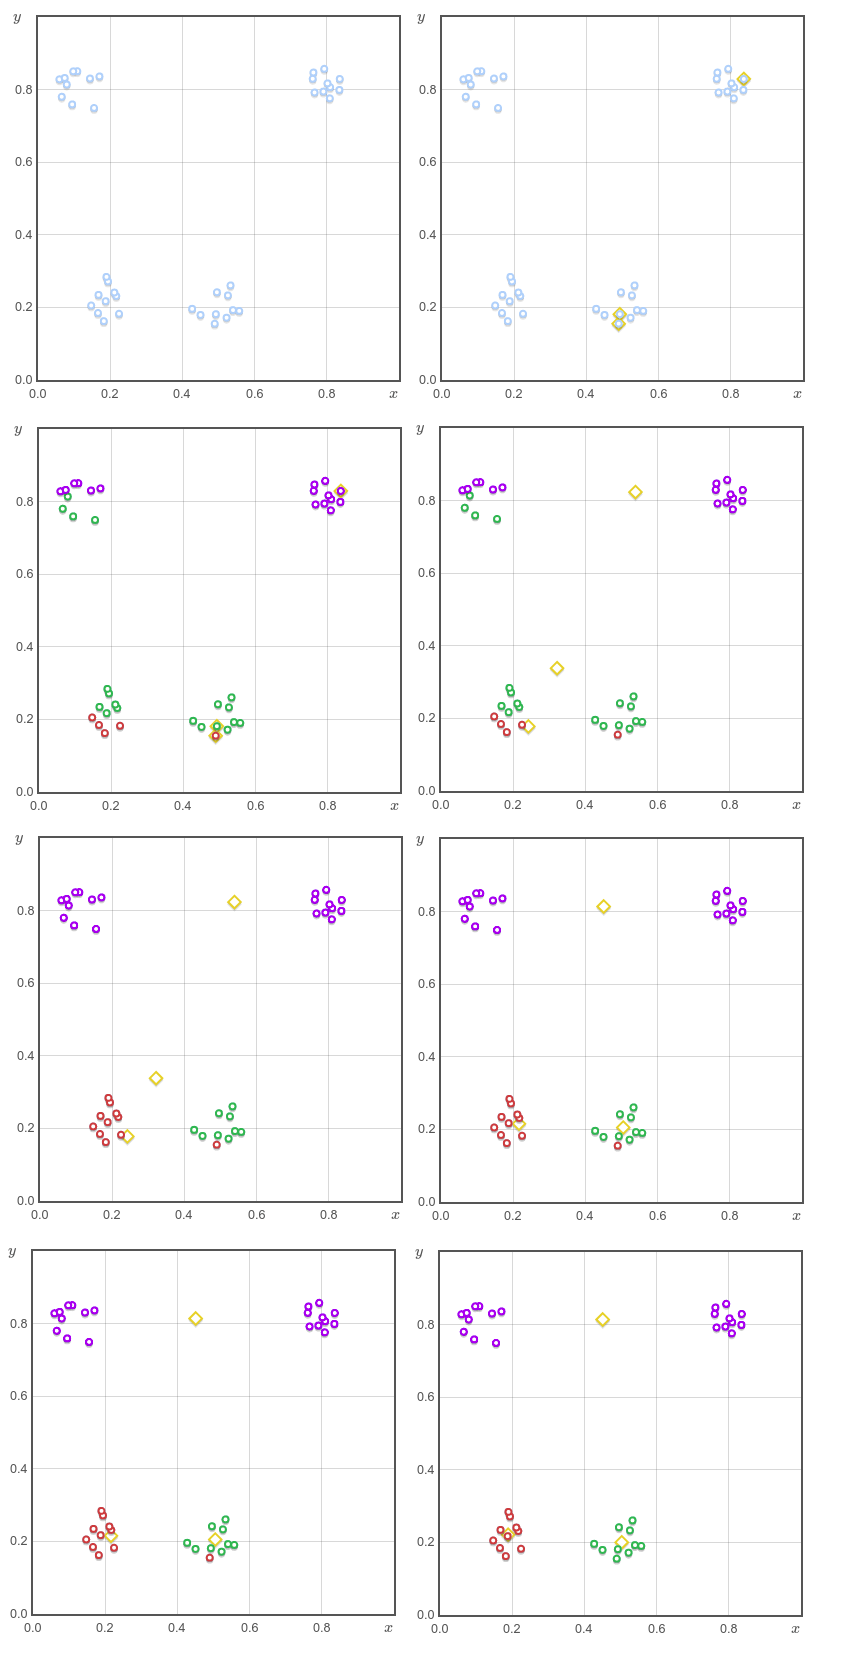
\includegraphics[width=0.5\textwidth]{img/k-means}}
\fonte{Extraído de \cite{kmeans-step}}
\end{figure}



A localização desses centróides deve ser o mais afastado entre si possível. A partir de uma posição inicial dos centróides, o próximo passo é, então, associar todos pontos do conjunto de dados com o centróide mais próximo. Com os pontos associados, recalcula-se k novos centróides como baricentros dos clusters anteriores, repetindo esses passos até que os novos centróides sejam gerados muito próximos do passo anterior. 





% ---
\section{Classificação}
% ---


\subsection{Regressão Linear}


A regressão linear é uma modelagem matemática \footnotemark \footnotetext{modelagem matemática é uma representação em fórmulas matemáticas que tentam descrever ou simular eventos e sistemas reais com o propósito de prever comportamentos} que permite descrever variáveis em função de outras. Ela pode ser representada como
\begin{equation}
  \label{eq:regressao_linear}
  \begin{aligned}
Y &= \hat{\beta_{0}} + \sum_{j=1}^{p} (X_{j}\hat{\beta_{j}}), 
  \end{aligned}  
\end{equation}
onde \begin{math}Y\end{math} representa uma variável dependente contínua, \begin{math}X_{j}\end{math} as variáveis independentes (contínuas, discretas ou binárias).

Para ajustar o modelo linear ao conjunto de dados, é possível utilizar diferentes maneiras. Um deles é método dos mínimos quadrados, uma técnica de otimização matemática que visa encontrar ajuste ótimo para um conjunto de dados por meio da minimização a soma dos quadrados das diferenças entre o valor estimado e os dados observados, representado por:

\begin{equation}
  \label{eq:minimos_quadrados}
  \begin{aligned}
G(\beta) &= \sum_{i=1}^{N} (y_{i}-x_{i}^{T}\beta)^{2}, 
  \end{aligned}  
\end{equation}

Assim, nosso problema passar a ser como descobrir \begin{math}\hat{\beta}\end{math} que minimize \ref{eq:minimos_quadrados}. Para calcular \begin{math}\hat{\beta}\end{math}, é possível utilizar a equação:

\begin{equation}
  \label{eq:solucao_minimos_quadrados}
  \begin{aligned}
\hat{\beta} &= (X^{T}X)^{-1}X^{T}y, 
  \end{aligned}  
\end{equation}

onde \begin{math} X \in \mathbb{R}^{N,p} \end{math} X representando uma matriz com cada linha sendo um vetor do conjunto de dados de entrada e \begin{math}y \in \mathbb{R}^{N}\end{math} um vetor que representa os dados de saída \footnotemark \footnotetext{inicialmente, esses dados devem vir do conjunto de treino}

Com a definição de \begin{math}\hat{\beta}\end{math}, é possível determinar uma reta que separa o conjunto de dad

\begin{figure}[!ht]
\centerline{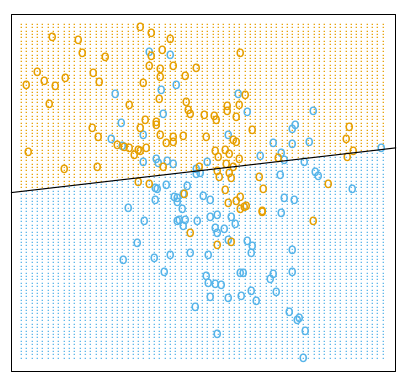
\includegraphics[width=0.5\textwidth]{img/hiperplano}}
\caption{Exemplo de classificação em 2 dimensões. Fonte: \cite{HASTIE}}
\end{figure}



 As classes estão representadas um variável binária (AZUL = 0, LARANJA = 1), ajustadas por uma regressão linear. A linha que separa os grupos foi definido por \begin{math}x^{T}\hat{\beta} = 0,5\end{math}. A área hachurada em laranja representa o espaço classificado por LARANJA enquanto a área em azul, classificado por AZUL

\subsection{Regressão Logística}

A regressão logística, assim como a regressão linear, também é um modelo matemático de predição de eventos usada para descrever dados e explicar a relação entre um conjunto de variáveis independentes e uma variável dependente. Contudo, enquanto na regressão linear a variável dependente é contínua, na regressão logística, ela é considerada uma variável categórica. Ela segue uma distribuição Bernoulli\footnotemark \footnotetext{distribuição de Bernoulli é uma modelagem de probabilidade que representa eventos binários cujas ocorrências são tratados como sucesso ou falha. Considerando que a probabilidade de ocorrer um sucesso é \begin{math}p\end{math}, então a probabilidade de ocorrer uma falha é \begin{math}1-p\end{math} } com uma probabilidade \begin{math}p\end{math} desconhecida. Assim, a regressão logística tem como objetivo estimar essa probabilidade \begin{math}p\end{math} desconhecida.

Para estimar essa probabilidade, a regressão logística usa as chances do evento ocorrer em cada variável independente, calculando a taxa dessas chances, dada pela equação:

\begin{equation}
  \label{eq:OR}
  \begin{aligned}
   OR &= \frac{P(sucesso)}{P(fracasso)}\\
     &= \frac{p}{1-p}
  \end{aligned}
\end{equation}

Utilizando inferência de estatística, podemos aplicar log em \ref{eq:OR}, ficando com:

\begin{equation}
  \label{eq:t}
  \begin{aligned}
    logit(p) &= ln\left ( \frac{p}{1-p} \right )
  \end{aligned}
\end{equation}

Tal transformação recebe o nome de logit. Ela é ajustada a função de predição, como numa análise de regressão linear, visto anteriormente. The predicted value of the logit is converted back into predicted odds via the inverse of the natural logarithm, namely the exponential function.

\begin{equation}
  \label{eq:t}
  \begin{aligned}
    logit^{-1}(\alpha) &= \frac{1}{1+e^{-\alpha}} &= \frac{e^{\alpha}}{1+e^{\alpha}}
  \end{aligned}
\end{equation}

Generalizando, temos:

\begin{equation}
  \label{eq:t}
  \begin{aligned}
    \log\left ( \frac{P(G = 1 | X = x)}{P(G = K | X = x)} \right ) &= \beta_{10}+\beta_{1}^{T}x\\
    \log\left ( \frac{P(G = 2 | X = x)}{P(G = K | X = x)} \right ) &= \beta_{20}+\beta_{2}^{T}x\\
    \log\left ( \frac{P(G = K-1 | X = x)}{P(G = K | X = x)} \right ) &= \beta_{(k-1)0}+\beta_{k-1}^{T}x,
  \end{aligned}
\end{equation}

onde o modelo é composto por K classes e K - 1 transformações logit. Utilizando a inversa da logit, temos:

\begin{equation}
  \label{eq:t}
  \begin{aligned}
    P(G = k | X = x) &= \frac{\exp \left ( \beta_{k0}+\beta_{k}^{T}x \right )}{1 + \sum_{\ell=1}^{K - 1}\exp \left ( \beta_{\ell0}+\beta_{\ell}^{T}x \right )}, k = 1, ..., K - 1\\
    P(G = K | X = x) &= \frac{1}{1 + \sum_{\ell=1}^{K - 1}\exp \left ( \beta_{\ell0}+\beta_{\ell}^{T}x \right )}
  \end{aligned}
\end{equation}


Thus, although the observed dependent variable in logistic regression is a zero-or-one variable, the logistic regression estimates the odds, as a continuous variable, that the dependent variable is a success (a case). In some applications the odds are all that is needed. In others, a specific yes-or-no prediction is needed for whether the dependent variable is or is not a case; this categorical prediction can be based on the computed odds of a success, with predicted odds above some chosen cutoff value being translated into a prediction of a success.




\begin{comment} 
\begin{citacao} 
\cite{HASTIE} \end{citacao}


, mas que leva em consideração as probabilidades de ocorrência desses eventos.
\end{comment}

Dessa forma, a regressão logística viabiliza a classificação das observações por meio da probabilidade estimada na categoria estudada.


% ---
\subsection{\emph{Random Forest}}


\subsubsection{Árvores}

% ---
Árvores são modelos presentes tanto em computação como estrutura de dados e em estatística como estrutura para tomadas de decisão. No contexto de \emph{Machine Learning}, a árvore de decisão refere-se a uma estrutura de modelo preditivo, um método de aprendizagem supervisionada não parametrizada utilizada para classificação (para variáveis categóricas) e regressão (variáveis métricas). Trata-se de um modelo de conjunto de decisões ou regras na qual estabelece um fluxo dentro de sua estrutura, definindo uma classificação ou uma predição. Para \citeonline[p. 305]{HASTIE}, as árvores permitem um particionamento do espaço em um conjunto regiões. Suponha que exista \begin{math}M\end{math} partição que possa ser divida em regiões \begin{math}R_{1}, R_{2}, ..., R_{M} \end{math} e que seja possível modelar a resposta para cada região com a constante \begin{math}c_{m}\end{math}, 

\begin{equation}
f(x) = \sum_{m=1}^{M}c_{m}I( x \in R_{m} ) .
\end{equation}

Para a repartição dessas regiões, são definidos critérios para decidir de qual lado o dado irá ficar na árvore. São estruturas de fácil interpretação pois, uma vez criado o modelo, percorrer os nós da árvore indica as características do dado.


\tikzset{
  treenode/.style = {shape=rectangle, rounded corners,
                     draw, align=center,
                     top color=white, bottom color=blue!20},
  root/.style     = {treenode, font=\Large, bottom color=purple!30},
  env/.style      = {treenode, font=\ttfamily\normalsize},
  dummy/.style    = {circle,draw}
}

\begin{figure}[!ht]
\caption{Exemplo de árvore classificadora}
\centering
        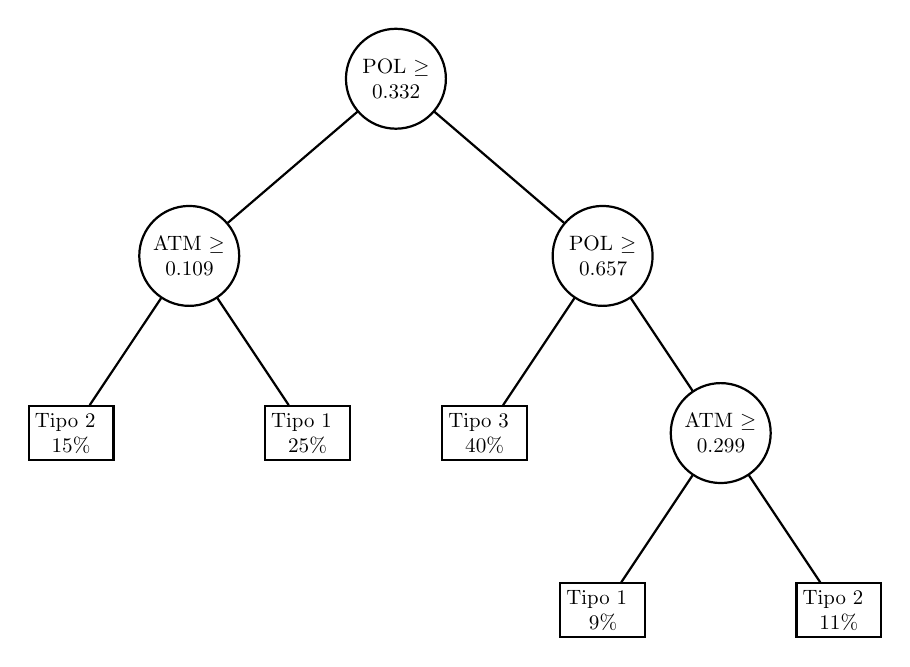
\begin{tikzpicture}[thick,scale=0.75, every node/.style={scale=0.75}]
\node [circle,draw,text width=1.2cm,align=center]{POL $\ge$ 0.332} [level distance=30mm,sibling distance=70mm]
child {node [circle,draw,text width=1.2cm,align=center] {ATM $\ge$ 0.109 } [level distance=30mm ,sibling distance=40mm]
child {node [rectangle,draw,text width=1.2cm,align=center] {Tipo 2\newline15\%}}
child {node [rectangle,draw,text width=1.2cm,align=center] {Tipo 1\newline25\%}}
}
child { node [circle,draw,text width=1.2cm,align=center]{ POL $\ge$ 0.657} [level distance=30mm ,sibling distance=40mm]
child {node [rectangle,draw,text width=1.2cm,align=center] {Tipo 3\newline40\%}}
child { node [circle,draw,text width=1.2cm,align=center]{ ATM $\ge$ 0.299 } [level distance=30mm ,sibling distance=40mm]
child {node [rectangle,draw,text width=1.2cm,align=center] {Tipo 1\newline9\%}}
child {node [rectangle,draw,text width=1.2cm,align=center] {Tipo 2\newline11\%}}
}
};
\end{tikzpicture}
\nota{Cada nó representa um atributo de um elemento da amostra. As folhas são consideradas a representação da classe a que uma observação pertence. Já o ramo é um conjunto de valores que reflete todas suas características e detalhes de um elemento}
\fonte{Criado pelo autor}
\end{figure}

\subsubsection{Árvore de regressão}

Para \citeonline[p. 307]{HASTIE}, árvores de regressão são utilizadas em problemas de predição. Assim, a variável de saída refere-se a uma variável numérica e contínua.

Assim como foi visto anteriormente, o algoritmo deve conseseguir decidir em quais variáveis e quais pontos as decisões serão tomadas, construindo a topologia da árvore.

No caso de uma regressão, poderia utiliza-se como critério de minimização a soma do mínimos quadrados \begin{math}\sum{ (y_{i} - f(x_{i}))^{2}}\end{math}, temos que o melhor \begin{math}\hat c_{m}\end{math} é exatamente a média para \begin{math}y_{i}\end{math} na região \begin{math}R_{m}\end{math}:

\begin{equation}
\label{eq:media}
\hat c_{m} = m\acute edia(y_{i} | x_{i} \in R_{m}) .
\end{equation}

Para encontrar a melhor partição, é necessário recorrer a um algoritmo guloso\footnotemark \footnotetext{\emph{algoritmo guloso} é um algoritmo que  busca a resolução de um problema elegendo sempre uma solução localmente ótima. Isto significa que, dentro de um conjunto de soluções possíveis numa determinada etapa da solução do problema, escolhe-se sempre a que traz o melhor resultado naquela situação, o que muitas vezes pode não levar a uma solução ótima global.}, uma vez que calcular utilizando os mínimos quadrados é computacionalmente inviável.

Seja \begin{math}j\end{math} uma variável de reparticionamento, $s$ um ponto de divisão. É possível definir um par de semi planos 

\begin{equation}
R_{1}(j,s) = {X | X_{j}\leq s} \quad \textrm{e} \quad R_{2}(j,s) = {X | X_{j}\textgreater s}) .
\end{equation}

Resultando a busca pela de \begin{math}s\end{math} e \begin{math}j\end{math} que resolva

\begin{equation}
\min_{j,s} \left [ \min_{c_{1}} \sum_{x_{i} \in R_{1} (j,s)} (y_{i} - c_{1})^{2} + \min_{c_{1}} \sum_{x_{i} \in R_{2} (j,s)}(y_{i} - c_{2})^{2} \right ] .
\end{equation} 


Mas como visto em \ref{eq:media}, temos que para qualquer $j$ e $s$, a minimização interna pode ser resolvida por:

\begin{equation}
\hat c_{1} = m\acute edia(y_{i} | x_{i} \in R_{1}(j,s)) \quad \textrm{e} \quad \hat c_{2} = m\acute edia(y_{i} | x_{i} \in R_{2}(j,s)) .
\end{equation} 

Este processo é repetido até que todas as regiões sejam descobertas.

\subsubsubsection{Árvore de classificação}

Para o caso de uma árvore de classificação, \citeonline[p. 308]{HASTIE} explica que o objetivo principal concentra-se em conseguir, a partir das variáveis independentes, efetuar a decisão em definir um classe para uma determinada entrada de dados. Logo, a saída é uma variável categórica.
Neste caso, utiliza-se como critério de decisão o índice de Gini\footnotemark \footnotetext{Índice de Gini mede a frequencia de que um elemento selecionado aleatoriamente de um conjunto é marcado de forma errada}
\begin{math}Gini(T) = 1 - \sum_{i=1}^{n}{ p_{i}^{2}}\end{math},
onde p é a proporção de observações de uma determinada classe para um dado nó.

\subsubsection{\emph{Bagging}}

As árvores vistas anteriormente são modelos interessantes de classificação mas possuem um problema: o resultado gerado por elas em geral possuem uma acurácia muito baixa quando a estrutura da árvore começa a crescer muito \cite[p. 312]{HASTIE}.
A proposta do \emph{Bagging} é criar subconjuntos dos dados, gerando diversas árvores que deverão executar a classificação. Esses modelos subconjuntos são gerados com reposição, ou seja, um mesmo dado pode estar presente em mais de um modelo no momento do treino. Cada árvore gerada fornecerá um modelo para a \emph{Random Forest} e um valor intermediário será adotado para os nós. 

\begin{figure*}[ht!]
    \centering
        \caption{Exemplo de composição da \emph{Random Forest}}
    \begin{subfigure}[t]{0.5\textwidth}
        \centering
        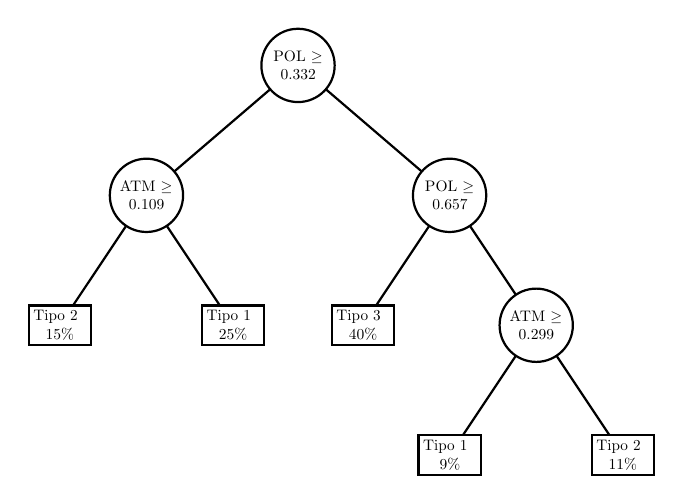
\begin{tikzpicture}[thick,scale=0.55, every node/.style={scale=0.55}]
\node [circle,draw,text width=1.2cm,align=center]{POL $\ge$ 0.332} [level distance=30mm,sibling distance=70mm]
child {node [circle,draw,text width=1.2cm,align=center] {ATM $\ge$ 0.109 } [level distance=30mm ,sibling distance=40mm]
child {node [rectangle,draw,text width=1.2cm,align=center] {Tipo 2\newline15\%}}
child {node [rectangle,draw,text width=1.2cm,align=center] {Tipo 1\newline25\%}}
}
child { node [circle,draw,text width=1.2cm,align=center]{ POL $\ge$ 0.657} [level distance=30mm ,sibling distance=40mm]
child {node [rectangle,draw,text width=1.2cm,align=center] {Tipo 3\newline40\%}}
child { node [circle,draw,text width=1.2cm,align=center]{ ATM $\ge$ 0.299 } [level distance=30mm ,sibling distance=40mm]
child {node [rectangle,draw,text width=1.2cm,align=center] {Tipo 1\newline9\%}}
child {node [rectangle,draw,text width=1.2cm,align=center] {Tipo 2\newline11\%}}
}
};
\end{tikzpicture}

        \caption{Configuração 1 da árvore de decisão}
    \end{subfigure}%
    ~ 
    \begin{subfigure}[t]{0.5\textwidth}
        \centering
        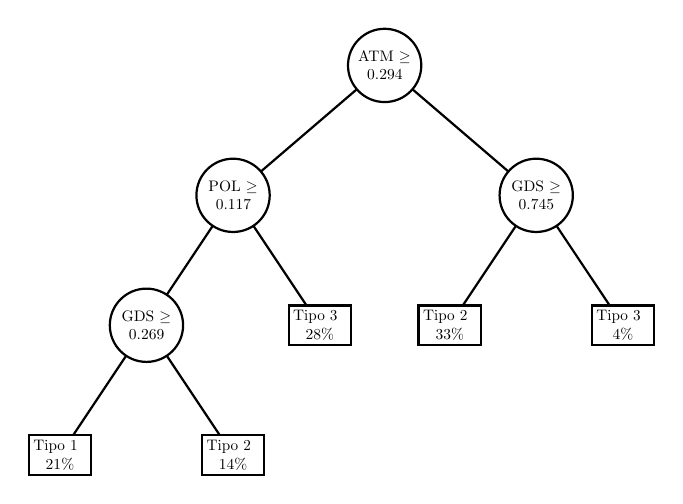
\begin{tikzpicture}[thick,scale=0.55, every node/.style={scale=0.55}]
\node [circle,draw,text width=1.2cm,align=center]{ATM $\ge$ 0.294} [level distance=30mm,sibling distance=70mm]
child { node [circle,draw,text width=1.2cm,align=center]{ POL $\ge$ 0.117 } [level distance=30mm ,sibling distance=40mm]
child { node [circle,draw,text width=1.2cm,align=center]{ GDS $\ge$ 0.269 } [level distance=30mm ,sibling distance=40mm]
child {node [rectangle,draw,text width=1.2cm,align=center] {Tipo 1\newline21\%}}
child {node [rectangle,draw,text width=1.2cm,align=center] {Tipo 2\newline14\%}}}
child {node [rectangle,draw,text width=1.2cm,align=center] {Tipo 3\newline28\%}}
}
child {node [circle,draw,text width=1.2cm,align=center] { GDS $\ge$ 0.745 } [level distance=30mm ,sibling distance=40mm]
child {node [rectangle,draw,text width=1.2cm,align=center] {Tipo 2\newline33\%}}
child {node [rectangle,draw,text width=1.2cm,align=center] {Tipo 3\newline4\%}}
};
\end{tikzpicture}
        \caption{Configuração 2 da árvore de decisão}
    \end{subfigure}
\fonte{Criado pelo autor}
\end{figure*}



% \begin{figure*}[t!]
%     \centering
%     \begin{subfigure}[t]{0.5\textwidth}
%         \centering
%         \begin{tikzpicture}[thick,scale=0.55, every node/.style={scale=0.55}]
% \node [circle,draw,text width=1.2cm,align=center]{POL $\ge$ 0.332} [level distance=30mm,sibling distance=70mm]
% child {node [circle,draw,text width=1.2cm,align=center] {ATM $\ge$ 0.109 } [level distance=30mm ,sibling distance=40mm]
% child {node [rectangle,draw,text width=1.2cm,align=center] {Tipo 2\newline15\%}}
% child {node [rectangle,draw,text width=1.2cm,align=center] {Tipo 1\newline25\%}}
% }
% child { node [circle,draw,text width=1.2cm,align=center]{ POL $\ge$ 0.657} [level distance=30mm ,sibling distance=40mm]
% child {node [rectangle,draw,text width=1.2cm,align=center] {Tipo 3\newline40\%}}
% child { node [circle,draw,text width=1.2cm,align=center]{ ATM $\ge$ 0.299 } [level distance=30mm ,sibling distance=40mm]
% child {node [rectangle,draw,text width=1.2cm,align=center] {Tipo 1\newline9\%}}
% child {node [rectangle,draw,text width=1.2cm,align=center] {Tipo 2\newline11\%}}
% }
% };
% \end{tikzpicture}

%         \caption{Configuração 1 da árvore de decisão}
%     \end{subfigure}%
%     ~ 
%     \begin{subfigure}[t]{0.5\textwidth}
%         \centering
%         \begin{tikzpicture}[thick,scale=0.55, every node/.style={scale=0.55}]
% \node [circle,draw,text width=1.2cm,align=center]{ATM $\ge$ 0.294} [level distance=30mm,sibling distance=70mm]
% child { node [circle,draw,text width=1.2cm,align=center]{ POL $\ge$ 0.117 } [level distance=30mm ,sibling distance=40mm]
% child { node [circle,draw,text width=1.2cm,align=center]{ GDS $\ge$ 0.269 } [level distance=30mm ,sibling distance=40mm]
% child {node [rectangle,draw,text width=1.2cm,align=center] {Tipo 1\newline21\%}}
% child {node [rectangle,draw,text width=1.2cm,align=center] {Tipo 2\newline14\%}}}
% child {node [rectangle,draw,text width=1.2cm,align=center] {Tipo 3\newline28\%}}
% }
% child {node [circle,draw,text width=1.2cm,align=center] { GDS $\ge$ 0.745 } [level distance=30mm ,sibling distance=40mm]
% child {node [rectangle,draw,text width=1.2cm,align=center] {Tipo 2\newline33\%}}
% child {node [rectangle,draw,text width=1.2cm,align=center] {Tipo 3\newline4\%}}
% };
% \end{tikzpicture}
%         \caption{Configuração 2 da árvore de decisão}
%     \end{subfigure}
%     \\
%     \centering
%     \begin{subfigure}[t]{0.5\textwidth}
%         \centering
%         \begin{tikzpicture}[thick,scale=0.55, every node/.style={scale=0.55}]
% \node [circle,draw,text width=1.2cm,align=center]{POL $\ge$ 0.332} [level distance=30mm,sibling distance=70mm]
% child {node [circle,draw,text width=1.2cm,align=center] {ATM $\ge$ 0.109 } [level distance=30mm ,sibling distance=40mm]
% child {node [rectangle,draw,text width=1.2cm,align=center] {Tipo 2\newline15\%}}
% child {node [rectangle,draw,text width=1.2cm,align=center] {Tipo 1\newline25\%}}
% }
% child { node [circle,draw,text width=1.2cm,align=center]{ POL $\ge$ 0.657} [level distance=30mm ,sibling distance=40mm]
% child {node [rectangle,draw,text width=1.2cm,align=center] {Tipo 3\newline40\%}}
% child { node [circle,draw,text width=1.2cm,align=center]{ ATM $\ge$ 0.299 } [level distance=30mm ,sibling distance=40mm]
% child {node [rectangle,draw,text width=1.2cm,align=center] {Tipo 1\newline9\%}}
% child {node [rectangle,draw,text width=1.2cm,align=center] {Tipo 2\newline11\%}}
% }
% };
% \end{tikzpicture}

%         \caption{Configuração 1 da árvore de decisão}
%     \end{subfigure}%
%     ~ 
%     \begin{subfigure}[t]{0.5\textwidth}
%         \centering
%         \begin{tikzpicture}[thick,scale=0.55, every node/.style={scale=0.55}]
% \node [circle,draw,text width=1.2cm,align=center]{ATM $\ge$ 0.294} [level distance=30mm,sibling distance=70mm]
% child { node [circle,draw,text width=1.2cm,align=center]{ POL $\ge$ 0.117 } [level distance=30mm ,sibling distance=40mm]
% child { node [circle,draw,text width=1.2cm,align=center]{ GDS $\ge$ 0.269 } [level distance=30mm ,sibling distance=40mm]
% child {node [rectangle,draw,text width=1.2cm,align=center] {Tipo 1\newline21\%}}
% child {node [rectangle,draw,text width=1.2cm,align=center] {Tipo 2\newline14\%}}}
% child {node [rectangle,draw,text width=1.2cm,align=center] {Tipo 3\newline28\%}}
% }
% child {node [circle,draw,text width=1.2cm,align=center] { GDS $\ge$ 0.745 } [level distance=30mm ,sibling distance=40mm]
% child {node [rectangle,draw,text width=1.2cm,align=center] {Tipo 2\newline33\%}}
% child {node [rectangle,draw,text width=1.2cm,align=center] {Tipo 3\newline4\%}}
% };
% \end{tikzpicture}
%         \caption{Configuração 2 da árvore de decisão}
%     \end{subfigure}
%     \caption{Configurações da árvore de decisão sobre subconjuntos distintos}
% \end{figure*}

Dessa forma, a solução para contornar esse problema foi a utilização dessa técnica nas árvores de decisões. Na \emph{Random Forest}, constrói-se uma árvore de classificação repetidamente usando amostras aleatórias do conjunto de dados. Por fim, o modelo final é recalculado.


\section{Tecnologias}

\subsection{\emph{Scikit Learn}}

O \emph{Scikit Learn} é um \emph{framework} desenvolvido em \emph{Python} voltado para \emph{Data Science}. Com mais de 30 contribuidores ativos, possui implementação de diversos algoritmos e de ferramentas que auxiliam desde a análise dos dados até a execução de tarefas como clusterização e classificação, além de disponibilizar integrações com programas visuais que facilitam muito a compreensão. 


\subsection{\emph{Apache Spark}}

O \emph{Apache Spark} é uma biblioteca com diversas ferramentas e viabiliza a escalabilidade da execução de algoritmos de \emph{Machine Learning}. É possível utilizar mais de linguagem de programação para desenvolver os programas. Neste trabalho, foi escolhido Scala.
Os algoritmos estudados (em especial o K Médias) são robustos e possuem uma grande carga de cálculos. Para bases grandes, o \emph{Scikit Learn} não é capaz de executar em tempo satisfatório. O \emph{Apache Spark}, por outro lado, oferece uma solução que possibilita uma maior rapidez na execução. Também é possível configurá-lo para que os algoritimos sejam executados em tempo real com alimentação contínua de dados. Contudo tal abordagem não será contemplada por não se tratar do foco do estudo.

\section{Avaliação dos algoritmos}

\subsection{Segmentação}

\subsubsection{Análise Descritiva}
A análise descritiva possibilita a descrição e sumarização dos dados de um conjunto. Há 2 tipos de medidas: a de tendência central e a de variabilidade ou dispersão. Entre as medidas de tendência central estão média, mediana e moda. Já para as medidas de variabilidade, existem o desvio padrão, variância, o valor máximo e mínimo e quantis.
Para a análise descritiva, pode-se utilizar gráficos como histogramas e boxplots que ajudam visualizar com clareza e caracterizar dos dados.


\subsection{Classificação}

\subsubsection{\emph{Cross Validation}}

A \emph{Cross Validation} é uma técnica que permite verificar a eficiência de um modelo preditivo \cite[p. 241]{HASTIE}. A idéia é particionar a base para se criar um modelo de treinamento e executar um teste. Essa partição é mutualmente exclusiva, ou seja, os dados que são usados para o treinamento não são reutilizados no teste. Neste caso, a \emph{Cross Validation} será executada nos algoritmos de classificação.


\subsubsection{Métricas}
O cálculo de métricas para os algoritmos são importantes para avaliar o desempenho da classificação. Cada métrica pode ser mais conveniente para cada tipo de problema ou natureza dos dados. Neste trabalho iremos abordar algumas métricas simples mas iremos fazer uma análise profunda.

\subsubsubsection{\emph{Precision}}

É calculado a partir da proporção dos verdadeiros positivos sobre a quantidade de todos elementos que foram classificados na mesma classe (soma dos verdadeiros positivos e falsos positivos)

\begin{equation}
  \label{eq:precision}
  \begin{aligned}
Precision &= \frac{VP}{VP + FP} 
  \end{aligned}  
\end{equation}

\subsubsubsection{\emph{Recall}}

É a proporção de elementos foram classificados corretamente em uma classe 
sobre a quantidade de todos elementos que realmente pertencem a esta classe mesmo que estejam em outras (soma dos verdadeiros positivos e falsos negativos). 

\begin{equation}
  \label{eq:precision}
  \begin{aligned}
Recall &= \frac{VP}{VP + FN} 
  \end{aligned}  
\end{equation}

\subsubsubsection{Falso Positivo}
O Falso Positivo corresponde aos elementos que foram classificados como pertencentes a uma dada classe mas que, quando na verdade, não pertencem a essa classe.

\subsubsubsection{\emph{F-measure}}
O F-measure é a média harmônica entre \emph{precision} e \emph{recall}. Trata-se de uma medida que consegue avaliar melhor conjunto de dados que possuem uma distribuição das classes desproporcionais. 

\begin{equation}
  \label{eq:precision}
  \begin{aligned}
F-measure &= (1 + \beta^{2})\frac{precision*recall}{\beta^{2}*precision + recall} 
  \end{aligned}  
\end{equation}

\subsubsection{\emph{Confusion Matrix}}
Trata-se de uma matriz quadrada na qual 
as colunas representam as classes as quais o elementos realmente pertencem enquanto as linhas representa a saída do classificador. Cada célula fornece a quantidade de elementos classificados.


%% ----------------------------------------------------------
% Anexos
% ----------------------------------------------------------

% ---
% Inicia os anexos
% ---
\begin{anexosenv}

% Imprime uma página indicando o início dos anexos
\partanexos


\chapter{Tabela de dados}

Para o caso do \emph{Loan Club}, nem todas as variáveis foram utilizadas. Isto se deve ao fato de que algumas das variáveis em questão são categóricas, outras que representam alguma descrição. Tratam-se de campos que provem informações substanciais mais que para o escopo deste trabalho foram desconsideradas. No caso de variáveis categóricas, seria possível uma conversão para variáveis \emph{dummies}, mas que para o caso do K Médias não devem ser consideradas. Já para os campos que possuem uma informação textual, existem algoritmos que podem fazer análises do conteúdo como \emph{word to vec} ou \emph{bag of words}.

 \label{tab:daypack}
    \begin{tabularx}{\textwidth}{p{.3\textwidth}X}
    \caption{Tabela de campos utilizados para a an\'alise do banco de dados \emph{Loan Club}}\\
    \toprule
    \textbf{Coluna} & \textbf{Descrição} \\[6pt]
    \midrule
    \endhead

funded\textunderscore amnt & Total do montante comprometido para aquele empr\'estimo at\'e este momento\\
funded\textunderscore amnt\textunderscore inv & Total do montante comprometido pelos investidores para aquele empr\'estimo at\'e este momento\\
grade & Nota atribu\'ida pelo \emph{Loan Club}\\
loan\textunderscore amnt & A quantia do empr\'estimo do mutu\'ario, podendo ter eventualmente descontos pelo departamento de cr\'edito\\
term & Quantidade de pagamentos do empr\'estimos que pode ser de 36 ou 60 meses\\
int\textunderscore rate & Taxa de juros do empr\'estimo\\
installment & Pagamento devido pelo tomador de empr\'estimo\\
annual\textunderscore inc & Renda anual relatada pelo devedor durante o cadastro\\
dti\textunderscore joint & A raz\~ao entre a quantia total de d\'ividas paga pelos co-mutu\'arios (desconsiderando hipotecas e o empr\'estimo feito pelo \emph{Loan Club}) dividido pela renda mensal dos co-mutu\'arios\\
delinq\textunderscore 2yrs & Incid\^encias de inadimpl\^encia (eventos ocorridos dentro de 30 dias) dentro de um per\'iodo de 2 anos\\
inq\textunderscore last\textunderscore 6mths & Quantidade de pedidos de empr\'estimos (excluindo carros e hipotecas)\\
open\textunderscore acc & N\'umero de linhas de cr\'editos abertas para o mutu\'ario\\
pub\textunderscore rec & N\'umero de \"derogatory public records\" (trata-se de um registro que pode ser considerado negativo para o mutu\'ario pois indica um risco e denegrindo sua reputa\c c\~ao e dificultando a possibilidade de aquisi\c c\~ao de outros produtos. Entre os valores, \'e poss\'ivel W e F\\
revol\textunderscore bal & Total de cr\'edito que n\~ao foi pago\\
total\textunderscore acc & N\'umero toral de linhas de cr\'editos usada pelo mutu\'ario\\
out\textunderscore prncp & Saldo devedor\\
out\textunderscore prncp\textunderscore inv & Saldo devedor sobre a por\c c\~ao de capital financiado por investidores\\
total\textunderscore pymnt & Pagamentos recebidos at\'e o momento presente sobre o valor financiado\\
total\textunderscore pymnt\textunderscore inv & Pagamentos recebidos at\'e o momento presente sobre o valor financiado pelo investidor\\
total\textunderscore rec\textunderscore int & Juros recebido at\'e a data presente\\
total\textunderscore rec\textunderscore late\textunderscore fee & Taxas de atraso recebido at\'e a presente data\\
total\textunderscore rec\textunderscore prncp & Capital financiado recebido at\'e a data presente\\
collection\textunderscore recovery\textunderscore fee & valor de imposto recuperado de \"charge off\" (declara\c c\~ao de n\~ao quita\c c\~ao de uma d\'ivida)\\
last\textunderscore pymnt\textunderscore amnt & Valor total de pagamento recebido\\
recoveries & valor bruto recuperado de \"charge off\" verificados \\
\bottomrule

\end{tabularx}


 \label{tab:daypack}
    \begin{tabularx}{\textwidth}{p{.3\textwidth}X}
    \caption{Tabela de campos disponíveis em \emph{Loan Club} e que n\~ao foram utilizados}\\
    \toprule
    \textbf{Coluna} & \textbf{Descrição} \\[6pt]
    \midrule
    \endhead

addr\textunderscore state & Estado de moradia do mutu\'ario\\
annual\textunderscore inc\textunderscore joint & Valor declarado no momento do cadastro da renda anual do co-mutu\'arios (um emprestimo eh realizado com co-mutuarios quando mais de uma pessao eh sao financiadas)\\
application\textunderscore type & Indica se o empr\'estimo ser\'a individual ou se ser\'a feito por mais de uma pessoa (co-mutu\'arios) \\
earliest\textunderscore cr\textunderscore line & M\^es mais recente em que o mutu\'ario abriu uma linha de cr\'edito\\
emp\textunderscore length & Per\'iodo em que o devedor est\'a empregado no trabalho atual, na qual 0 representa menos de 1 ano e 10 pode ser de 10 a mais anos \\
emp\textunderscore title & Descri\c c\~ao breve do emprego do devedor\\
fico\textunderscore range\textunderscore high & Limite superior do score proveniente do FICO a qual o devedor est\'a enquadrado\\
fico\textunderscore range\textunderscore low & Limite inferior do score proveniente do FICO a qual o devedor est\'a enquadrado\\
home\textunderscore ownership & Indica o status do tipo de moradia do tomador de empr\'estimo RENT (aluguel), OWN (casa pr\'opria), MORTGAGE (hipoteca), OTHER (outros)\\
id & vari\'avel de identifica\c c\~ao de cada cliente da \emph{Loan Club}\\
initial\textunderscore list\textunderscore status & Status inicial e interno da \emph{Loan Club} do mutu\'ario. Varia entre W e F\\
is\textunderscore inc\textunderscore v & Indica se a renda foi verificada pela \emph{Loan Club} ou n\~ao ou se a fonte de renda foi verificada\\
issue\textunderscore d & M\^es no qual o empr\'estimo foi financiado\\
last\textunderscore credit\textunderscore pull\textunderscore d & O m\^es mais recente desde que o mutu\'ario adquiriu cr\'edito no financiamento\\
last\textunderscore fico\textunderscore range\textunderscore high & O limite superior do \'ultimo score do FICO em que o mutu\'ario foi classificado\\
last\textunderscore fico\textunderscore range\textunderscore low & O limite inferior do \'ultimo score do FICO em que o mutu\'ario foi classificado\\
last\textunderscore pymnt\textunderscore d & \'Ultimo m\^es em que foi recebido um pagamento\\
loan\textunderscore status & Status atual do empr\'estimo\\
mths\textunderscore since\textunderscore last\textunderscore delinq & N\'umero de meses desde a \'ultima inadimpl\^encia do mutu\'ario\\
mths\textunderscore since\textunderscore last\textunderscore major\textunderscore derog & Meses desde a pior nota (em um per\'iodo de 90 dias)\\
mths\textunderscore since\textunderscore last\textunderscore record & N\'unmero de meses desde o \'ultimo registro de informa\c c\~oes p\'ublicas (anteced\^encia criminal)\\
next\textunderscore pymnt\textunderscore d & Data do pr\'oximo pagamento\\
policy\textunderscore code & C\'odigo interno da \emph{Loan Club}, variando entre 1 e 2\\
purpose & Categoria escolhida pelo mutu\'ario no momento da solicita\c c\~ao do cr\'edito\\
pymnt\textunderscore plan & Indica se o pagamento do plano est\'a em dia\\
revol\textunderscore util & Taxa de utiliza\c c\~ao da linha de cr\'edito (revolving account)\\
sub\textunderscore grade & Sub nota atribu\'ida pelo Loan Club\\
title & Tipo de empr\'estimo realizado pelo mutu\'ario\\
verified\textunderscore status\textunderscore joint & Indica se a renda dos co-mutu\'arios foi verificada pela \emph{Loan Club}, se n\~ao foi ou se a fonte de renda foi verificada\\
zip\textunderscore code & Os primeiros 3 n\'umeros de c\'odigo postal fornecida pelo mutu\'ario\\
open\textunderscore acc\textunderscore 6m & N\'umero de neg\'ocios abertos nos \'ultimos 6 meses\\
open\textunderscore il\textunderscore 6m & N\'umero de opera\c c\~oes de financiamento ativos \\
open\textunderscore il\textunderscore 12m & N\'umero de contas de opera\c c\~oes de financiamento abertas nos \'ultimos 12 meses\\
open\textunderscore il\textunderscore 24m & N\'umero de contas de opera\c c\~oes de financiamento abertas nos \'ultimos 24 meses\\
mths\textunderscore since\textunderscore rcnt\textunderscore il & Quantidade de meses desde que a mais recente conta de opera\c c\~oes de financiamento aberta\\
total\textunderscore bal\textunderscore il & Saldo total de todas as installment accounts\\
il\textunderscore util & Raz\~ao entre o total de saldo sobre o limite de cr\'edito para todas as installment accounts\\
open\textunderscore rv\textunderscore 12m & Quantidade de contas (revolving accounts) nos \'ultimos 12 meses\\
open\textunderscore rv\textunderscore 24m & Quantidade de contas (revolving accounts) abertas nos \'ultimos 24 meses\\
max\textunderscore bal\textunderscore bc & Saldo atual de todas as contas abertas (revolving accounts)\\
all\textunderscore util & Saldo de limite de cr\'editos para todas as opera\c c\~oes\\
total\textunderscore rev\textunderscore hi\textunderscore lim & Total limite de revolving cr\'editos\\
inq\textunderscore fi & N\'umero de solicita\c c\~oes de cr\'edito para finan\c cas pessoais\\
total\textunderscore cu\textunderscore tl & N\'umero de neg\'ocios financeiros\\

acc\textunderscore now\textunderscore delinq & N\'umero de contas nas quais o mutu\'ario est\'a agora inadimplente\\
tot\textunderscore coll\textunderscore amt & Saldo total de collection accounts \\
tot\textunderscore cur\textunderscore bal & Saldo total de todas as contas do mutuário \\
\bottomrule

\end{tabularx}


\chapter{Análise dos \emph{clusters} vs \emph{grades}}

Durante os estudos, foram feitas algumas análises com \emph{boxplots} para entender os \emph{clusters} gerados. Também foram feitos uma comparação com os clientes de acordo com os seus grades para ver se era possível encontrar algum padrão nos registros. Detectar padrões de dados é uma tarefa complexa e visto que não se trata do foco do trabalho, o estudo limitou-se a verificar apenas alguma ocorrência de padrão.

Nos anexos, estão os outros \emph{boxplots} gerados que não constam na parte de Resultados.

\clearpage

\begin{figure*}[t!]
    \centering
        \caption{\emph{Boxplots} de collection\textunderscore recovery\textunderscore fee }
        \begin{subfigure}[t]{0.45\textwidth}
            \centering
            \caption{Cluster }

            \centerline{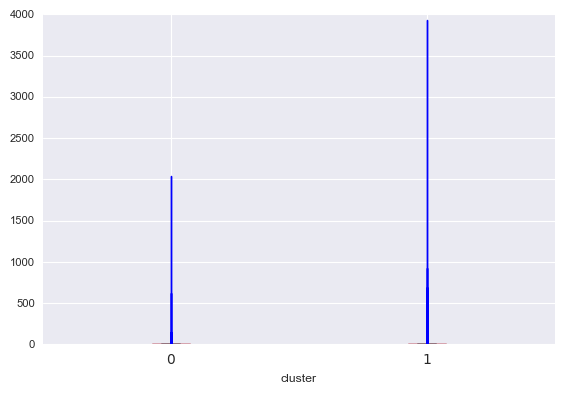
\includegraphics[width=1\textwidth]{img/collection_recovery_fee_by_cluster}}
        \end{subfigure}%
        ~ 
        \begin{subfigure}[t]{0.45\textwidth}
            \centering
            \caption{Grade}
   
            \centerline{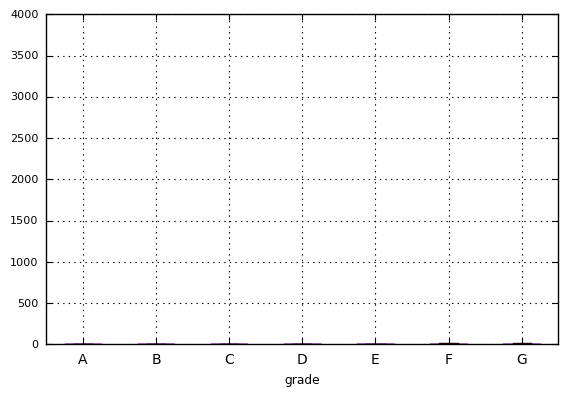
\includegraphics[width=1\textwidth]{img/collection_recovery_fee_by_grade}}

        \end{subfigure}
        \\
                \caption{\emph{Boxplots} de funded\textunderscore amnt}
        \begin{subfigure}[t]{0.45\textwidth}
            \centering

            \centerline{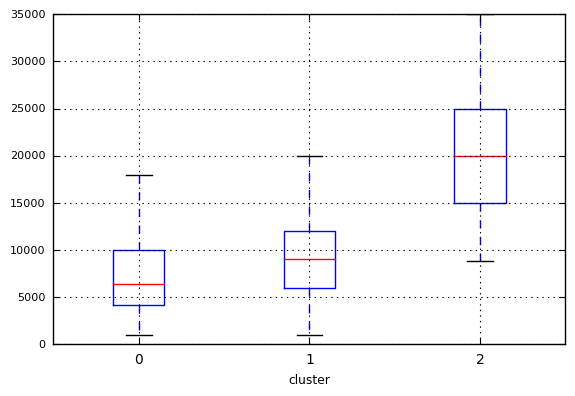
\includegraphics[width=1.05\textwidth]{img/funded_amnt_by_cluster}}
        \end{subfigure}%
        ~ 
        \begin{subfigure}[t]{0.45\textwidth}
            \centering
   
            \centerline{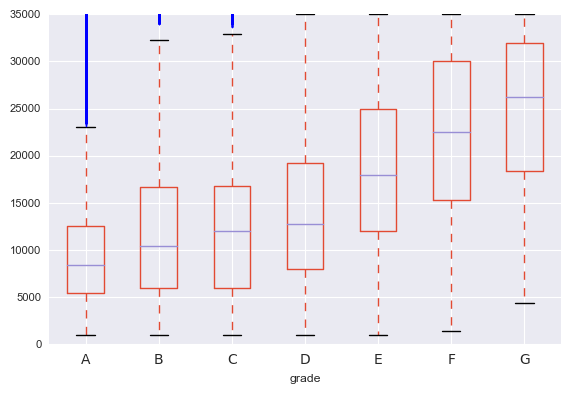
\includegraphics[width=1.05\textwidth]{img/funded_amnt_by_grade}}

        \end{subfigure}

\end{figure*}

\begin{figure*}[t!]
    \centering
        \caption{\emph{Boxplots} de funded\textunderscore amnt\textunderscore inv }
        \begin{subfigure}[t]{0.45\textwidth}
 
            \centerline{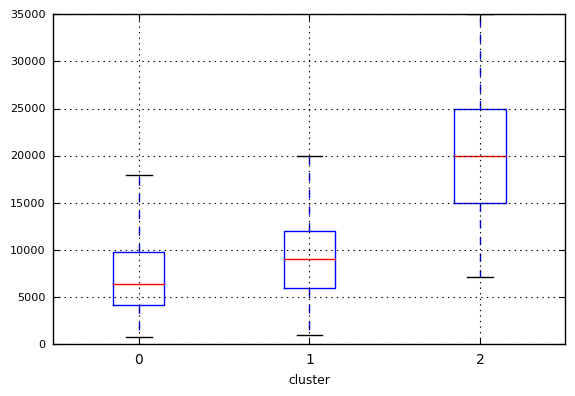
\includegraphics[width=1\textwidth]{img/funded_amnt_inv_by_cluster}}
        \end{subfigure}%
        ~ 
        \begin{subfigure}[t]{0.45\textwidth}
            \centerline{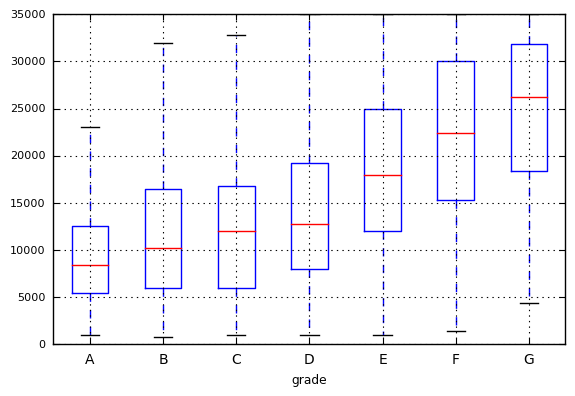
\includegraphics[width=1\textwidth]{img/funded_amnt_inv_by_grade}}

        \end{subfigure}
        \\
                \caption{\emph{Boxplots} de installment}
        \begin{subfigure}[t]{0.45\textwidth}
            \centering

            \centerline{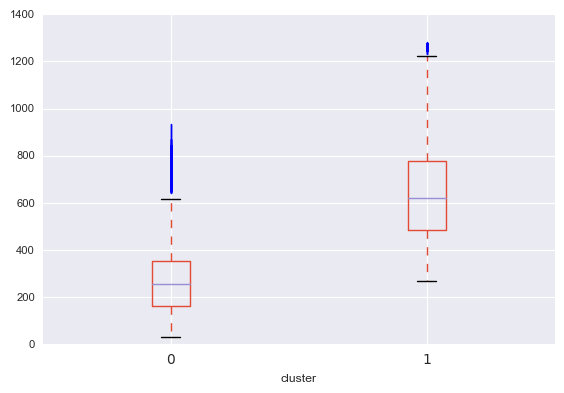
\includegraphics[width=1.05\textwidth]{img/installment_by_cluster}}
        \end{subfigure}%
        ~ 
        \begin{subfigure}[t]{0.45\textwidth}
            \centering
   
            \centerline{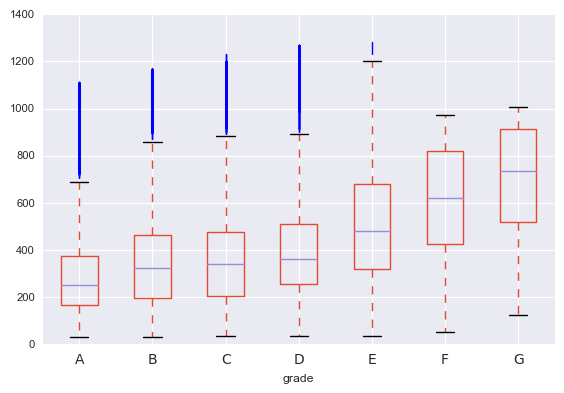
\includegraphics[width=1.05\textwidth]{img/installment_by_grade}}

        \end{subfigure}



\end{figure*}

\begin{figure*}[t!]
    \centering
        \caption{\emph{Boxplots} de term\textunderscore float\textunderscore fee }
        \begin{subfigure}[t]{0.45\textwidth}
            \centering

            \centerline{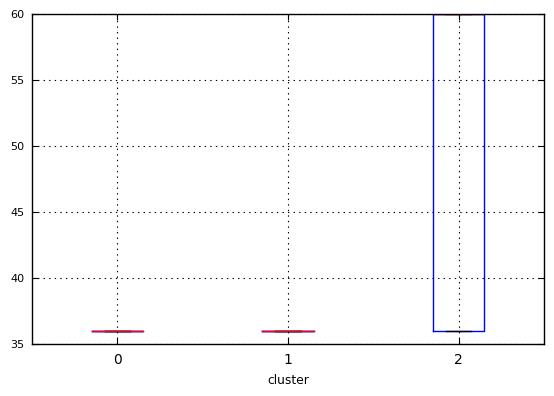
\includegraphics[width=1\textwidth]{img/term_float_by_cluster}}
        \end{subfigure}%
        ~ 
        \begin{subfigure}[t]{0.45\textwidth}
            \centering
   
            \centerline{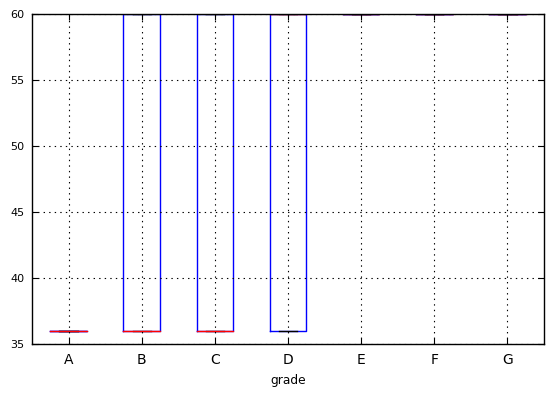
\includegraphics[width=1\textwidth]{img/term_float_by_grade}}

        \end{subfigure}
        \\
                \caption{\emph{Boxplots} de loan\textunderscore amnt}
        \begin{subfigure}[t]{0.45\textwidth}
            \centering

            \centerline{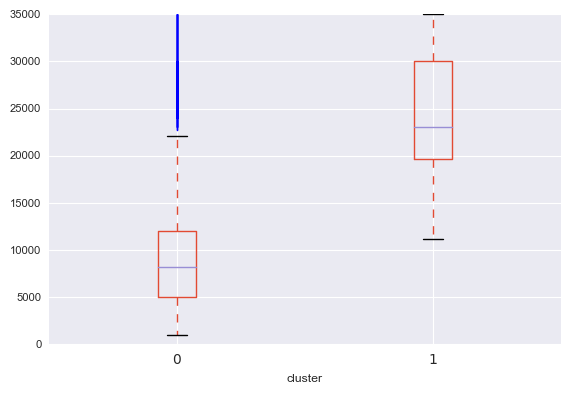
\includegraphics[width=1.05\textwidth]{img/loan_amnt_by_cluster}}
        \end{subfigure}%
        ~ 
        \begin{subfigure}[t]{0.45\textwidth}
            \centering
   
            \centerline{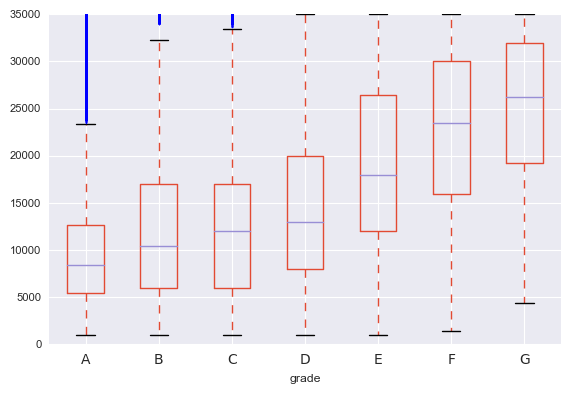
\includegraphics[width=1.05\textwidth]{img/loan_amnt_by_grade}}

        \end{subfigure}
\\
                \caption{\emph{Boxplots} de int\textunderscore rate\textunderscore float}
        \begin{subfigure}[t]{0.45\textwidth}
            \centering

            \centerline{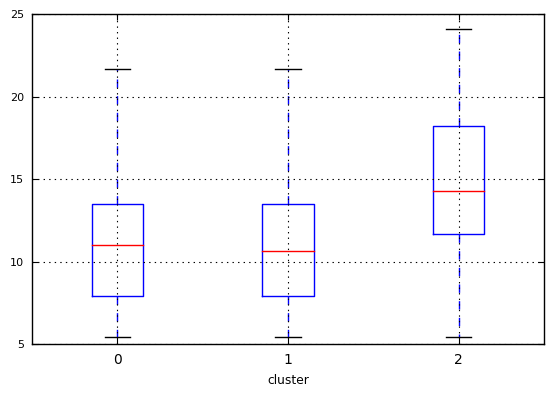
\includegraphics[width=1.05\textwidth]{img/int_rate_float_by_cluster}}
        \end{subfigure}%
        ~ 
        \begin{subfigure}[t]{0.45\textwidth}
            \centering
   
            \centerline{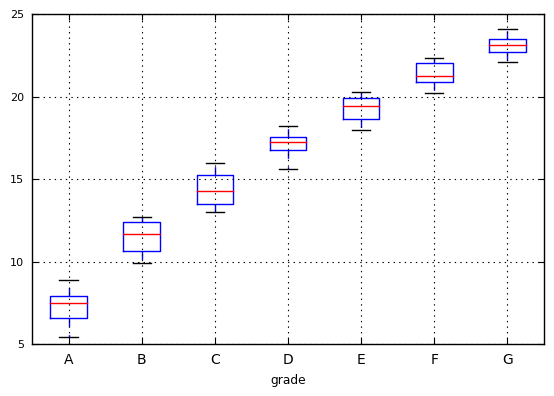
\includegraphics[width=1.05\textwidth]{img/int_rate_float_by_grade}}

        \end{subfigure}
\end{figure*}



\begin{figure*}[t!]
    \centering
        \caption{\emph{Boxplots} de annual\textunderscore inc }
        \begin{subfigure}[t]{0.45\textwidth}
            \centering

            \centerline{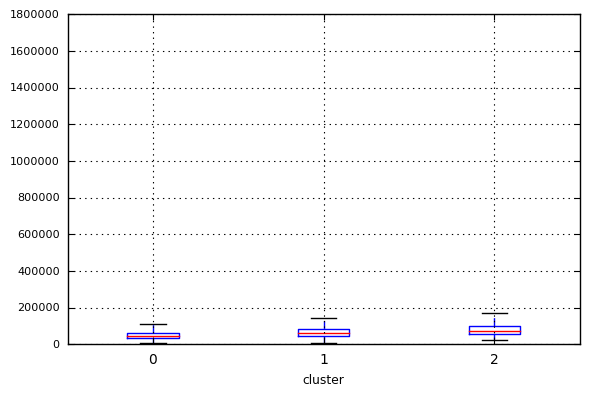
\includegraphics[width=1\textwidth]{img/annual_inc_by_cluster}}
        \end{subfigure}%
        ~ 
        \begin{subfigure}[t]{0.45\textwidth}
            \centering
   
            \centerline{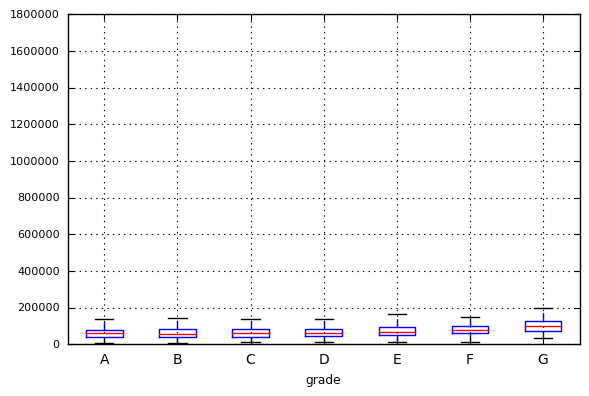
\includegraphics[width=1\textwidth]{img/annual_inc_by_grade}}

        \end{subfigure}
        \\
                \caption{\emph{Boxplots} de delinq\textunderscore 2yrs}
        \begin{subfigure}[t]{0.45\textwidth}
            \centering

            \centerline{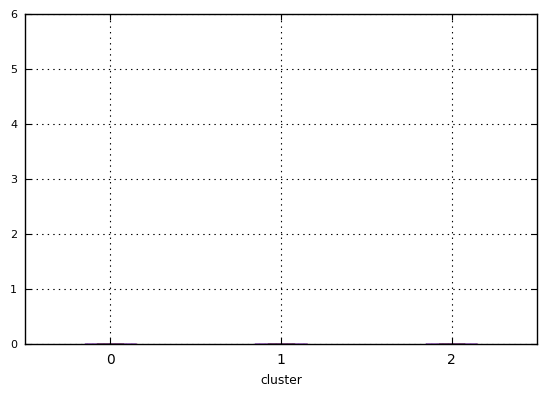
\includegraphics[width=1.05\textwidth]{img/delinq_2yrs_by_cluster}}
        \end{subfigure}%
        ~ 
        \begin{subfigure}[t]{0.45\textwidth}
            \centering
   
            \centerline{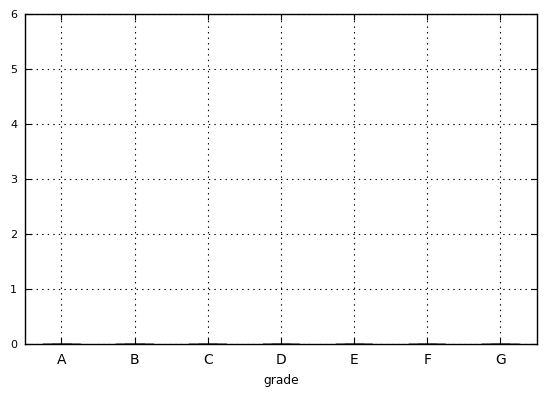
\includegraphics[width=1.05\textwidth]{img/delinq_2yrs_by_grade}}

        \end{subfigure}
\\
                \caption{\emph{Boxplots} de recoveries}
        \begin{subfigure}[t]{0.45\textwidth}
            \centering

            \centerline{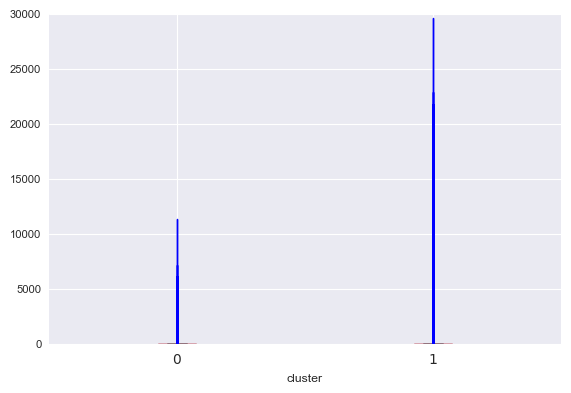
\includegraphics[width=1.05\textwidth]{img/recoveries_by_cluster}}
        \end{subfigure}%
        ~ 
        \begin{subfigure}[t]{0.45\textwidth}
            \centering
   
            \centerline{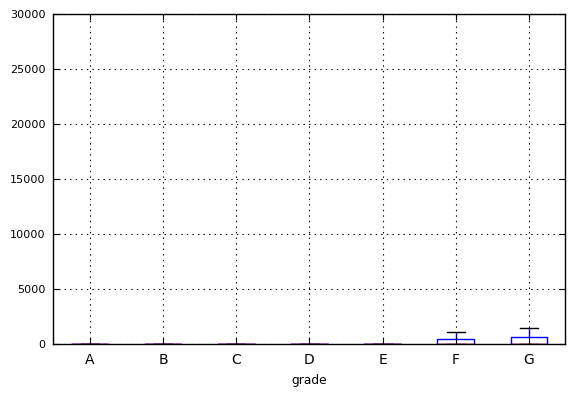
\includegraphics[width=1.05\textwidth]{img/recoveries_by_grade}}

        \end{subfigure}
\end{figure*}


\begin{figure*}[t!]
    \centering
        \caption{\emph{Boxplots} de open\textunderscore acc }
        \begin{subfigure}[t]{0.45\textwidth}
            \centering

            \centerline{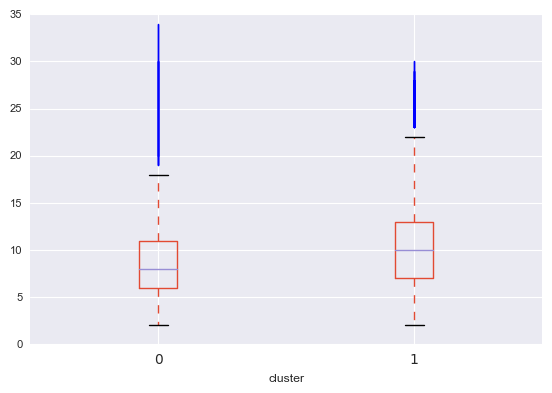
\includegraphics[width=1\textwidth]{img/open_acc_by_cluster}}
        \end{subfigure}%
        ~ 
        \begin{subfigure}[t]{0.45\textwidth}
            \centering
   
            \centerline{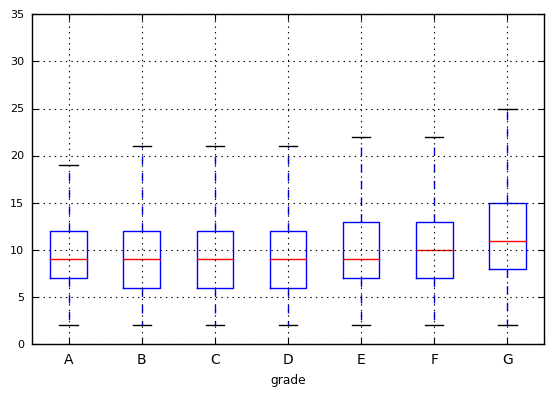
\includegraphics[width=1\textwidth]{img/open_acc_by_grade}}

        \end{subfigure}
        \\
                \caption{\emph{Boxplots} de pub\textunderscore rec}
        \begin{subfigure}[t]{0.45\textwidth}
            \centering

            \centerline{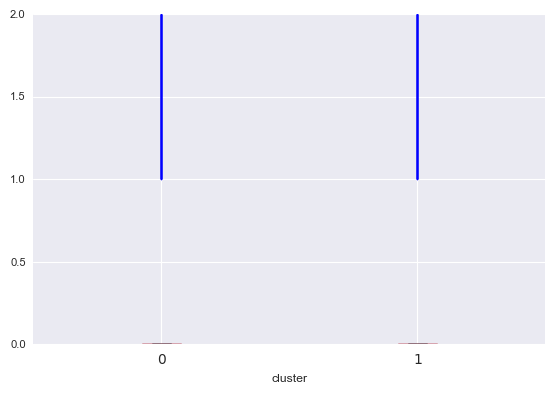
\includegraphics[width=1.05\textwidth]{img/pub_rec_by_cluster}}
        \end{subfigure}%
        ~ 
        \begin{subfigure}[t]{0.45\textwidth}
            \centering
   
            \centerline{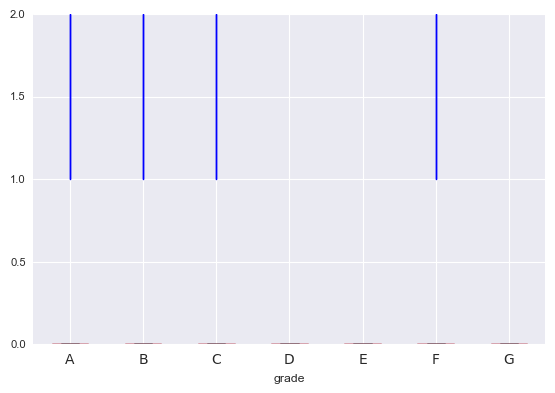
\includegraphics[width=1.05\textwidth]{img/pub_rec_by_grade}}

        \end{subfigure}
\\
                \caption{\emph{Boxplots} de inq\textunderscore last\textunderscore 6mths}
        \begin{subfigure}[t]{0.45\textwidth}
            \centering

            \centerline{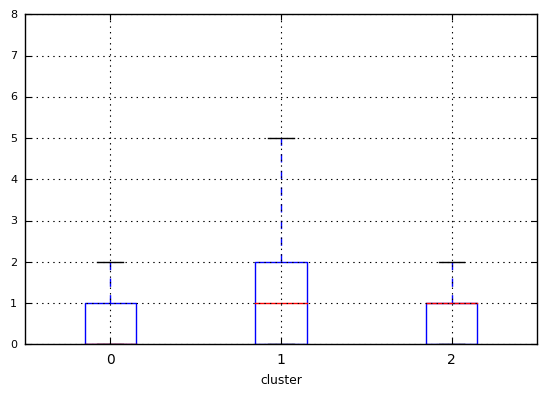
\includegraphics[width=1.05\textwidth]{img/inq_last_6mths_by_cluster}}
        \end{subfigure}%
        ~ 
        \begin{subfigure}[t]{0.45\textwidth}
            \centering
   
            \centerline{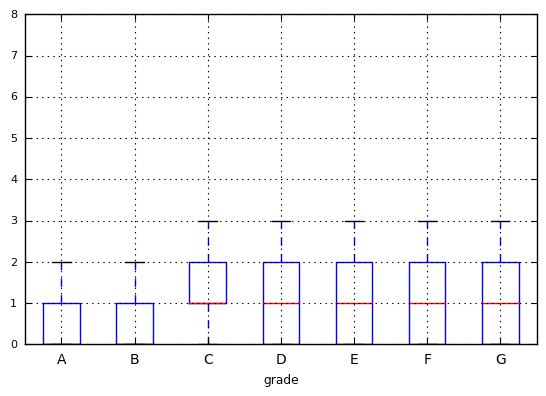
\includegraphics[width=1.05\textwidth]{img/inq_last_6mths_by_grade}}

        \end{subfigure}
\end{figure*}

\begin{figure*}[t!]
    \centering
        \caption{\emph{Boxplots} de revol\textunderscore bal }
        \begin{subfigure}[t]{0.45\textwidth}
            \centering

            \centerline{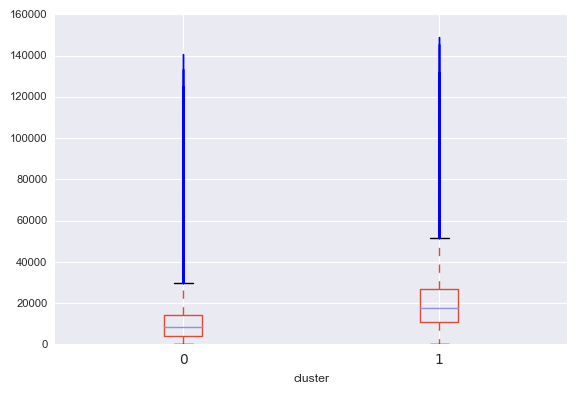
\includegraphics[width=1\textwidth]{img/revol_bal_by_cluster}}
        \end{subfigure}%
        ~ 
        \begin{subfigure}[t]{0.45\textwidth}
            \centering
   
            \centerline{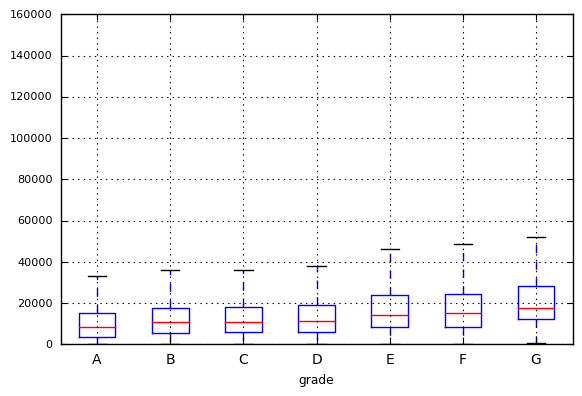
\includegraphics[width=1\textwidth]{img/revol_bal_by_grade}}

        \end{subfigure}
        \\
                \caption{\emph{Boxplots} de total\textunderscore acc}
        \begin{subfigure}[t]{0.45\textwidth}
            \centering

            \centerline{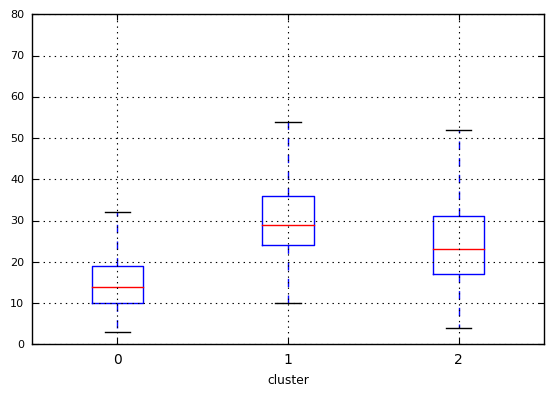
\includegraphics[width=1.05\textwidth]{img/total_acc_by_cluster}}
        \end{subfigure}%
        ~ 
        \begin{subfigure}[t]{0.45\textwidth}
            \centering
   
            \centerline{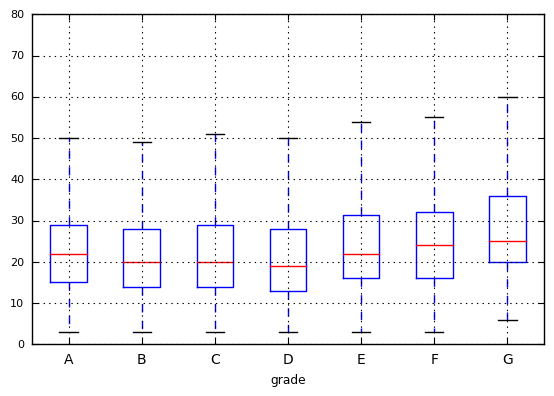
\includegraphics[width=1.05\textwidth]{img/total_acc_by_grade}}

        \end{subfigure}
\\
                \caption{\emph{Boxplots} de out\textunderscore prncp}
        \begin{subfigure}[t]{0.45\textwidth}
            \centering

            \centerline{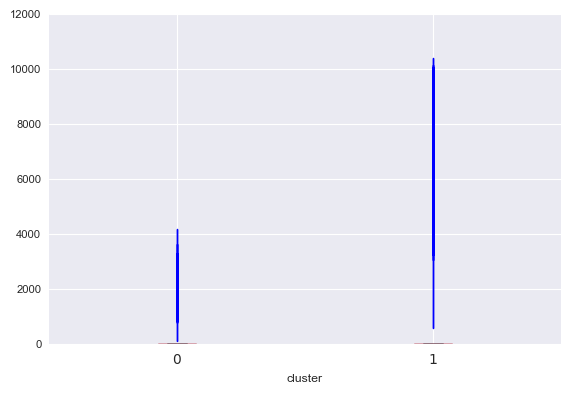
\includegraphics[width=1.05\textwidth]{img/out_prncp_by_cluster}}
        \end{subfigure}%
        ~ 
        \begin{subfigure}[t]{0.45\textwidth}
            \centering
   
            \centerline{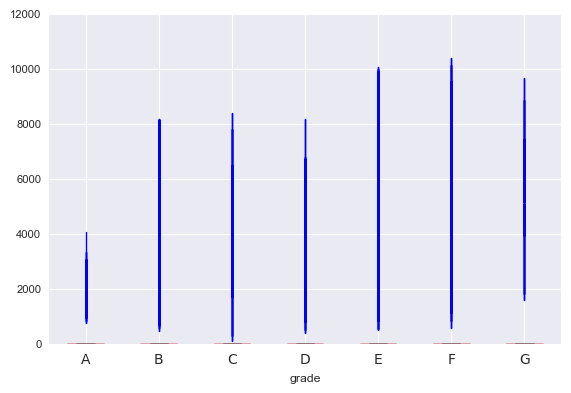
\includegraphics[width=1.05\textwidth]{img/out_prncp_by_grade}}

        \end{subfigure}
\end{figure*}


\begin{figure*}[t!]
    \centering
        \caption{\emph{Boxplots} de total\textunderscore pymnt }
        \begin{subfigure}[t]{0.45\textwidth}
            \centering

            \centerline{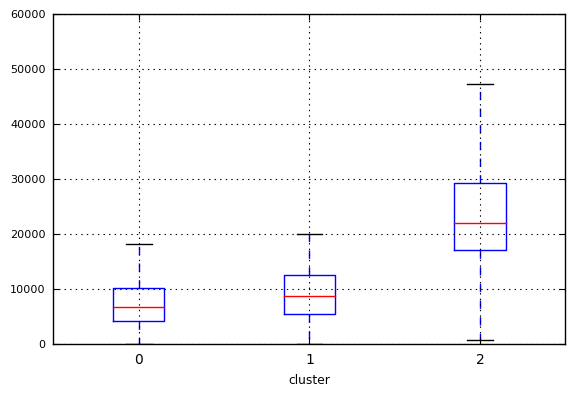
\includegraphics[width=1\textwidth]{img/total_pymnt_by_cluster}}
        \end{subfigure}%
        ~ 
        \begin{subfigure}[t]{0.45\textwidth}
            \centering
   
            \centerline{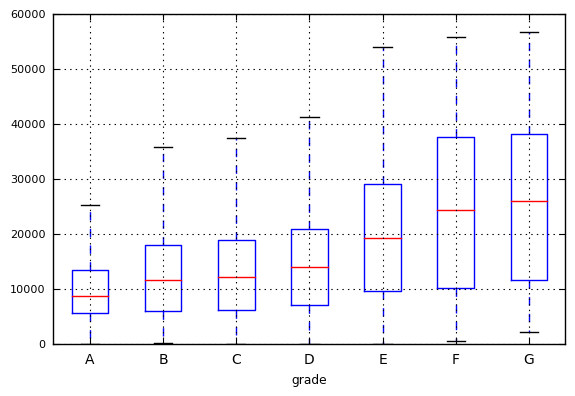
\includegraphics[width=1\textwidth]{img/total_pymnt_by_grade}}

        \end{subfigure}
        \\
                \caption{\emph{Boxplots} de out\textunderscore prncp\textunderscore inv}
        \begin{subfigure}[t]{0.45\textwidth}
            \centering

            \centerline{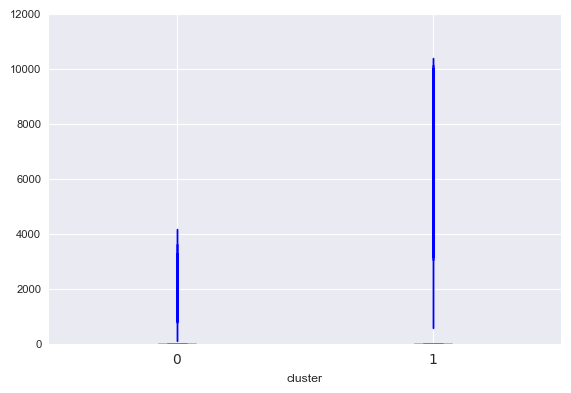
\includegraphics[width=1.05\textwidth]{img/out_prncp_inv_by_cluster}}
        \end{subfigure}%
        ~ 
        \begin{subfigure}[t]{0.45\textwidth}
            \centering
   
            \centerline{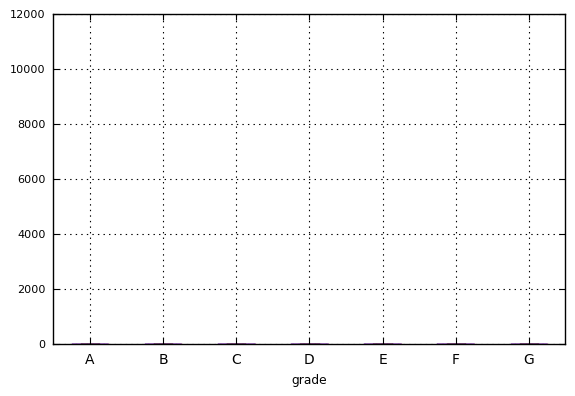
\includegraphics[width=1.05\textwidth]{img/out_prncp_inv_by_grade}}

        \end{subfigure}
\\
                \caption{\emph{Boxplots} de total\textunderscore rec\textunderscore int }
        \begin{subfigure}[t]{0.45\textwidth}
            \centering

            \centerline{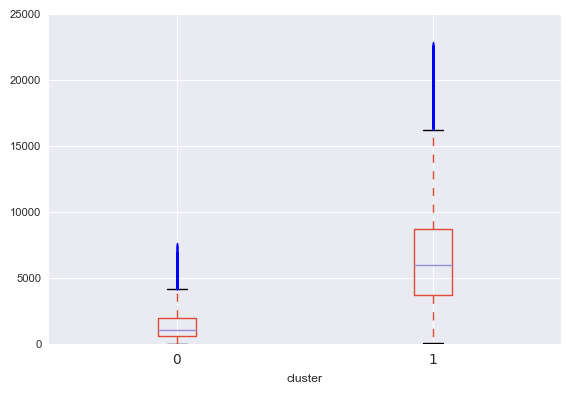
\includegraphics[width=1.05\textwidth]{img/total_rec_int_by_cluster}}
        \end{subfigure}%
        ~ 
        \begin{subfigure}[t]{0.45\textwidth}
            \centering
   
            \centerline{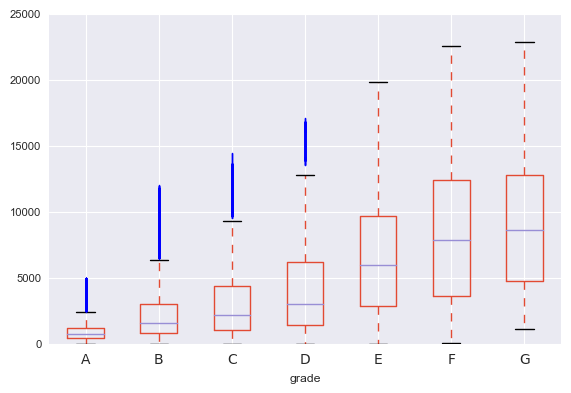
\includegraphics[width=1.05\textwidth]{img/total_rec_int_by_grade}}

        \end{subfigure}
\end{figure*}



\begin{figure*}[t!]
    \centering
        \caption{\emph{Boxplots} de total\textunderscore pymnt\textunderscore inv }
        \begin{subfigure}[t]{0.45\textwidth}
            \centering

            \centerline{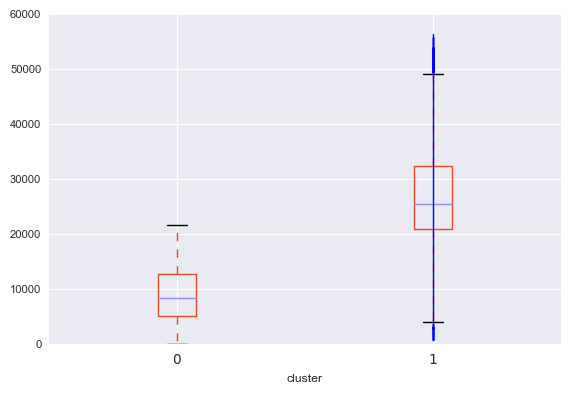
\includegraphics[width=1\textwidth]{img/total_pymnt_inv_by_cluster}}
        \end{subfigure}%
        ~ 
        \begin{subfigure}[t]{0.45\textwidth}
            \centering
   
            \centerline{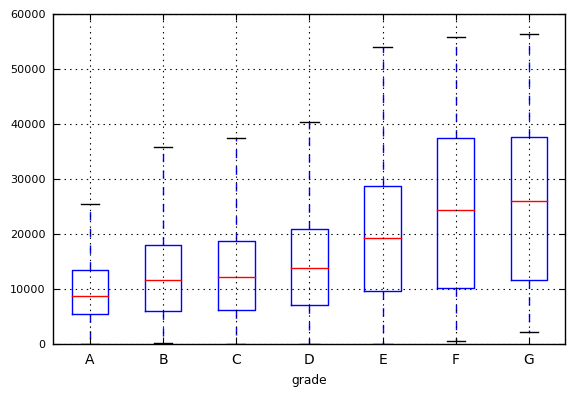
\includegraphics[width=1\textwidth]{img/total_pymnt_inv_by_grade}}

        \end{subfigure}
        \\
                \caption{\emph{Boxplots} de last\textunderscore pymnt\textunderscore amnt}
        \begin{subfigure}[t]{0.45\textwidth}
            \centering

            \centerline{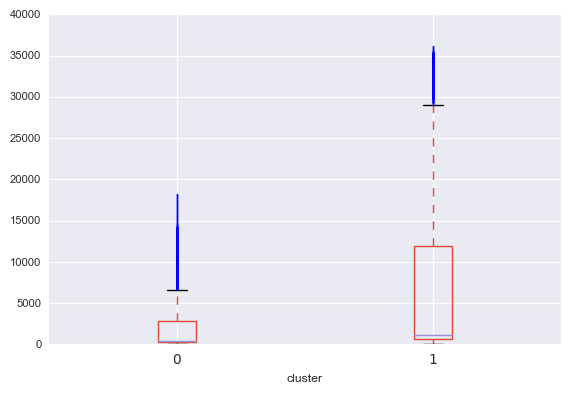
\includegraphics[width=1.05\textwidth]{img/last_pymnt_amnt_by_cluster}}
        \end{subfigure}%
        ~ 
        \begin{subfigure}[t]{0.45\textwidth}
            \centering
   
            \centerline{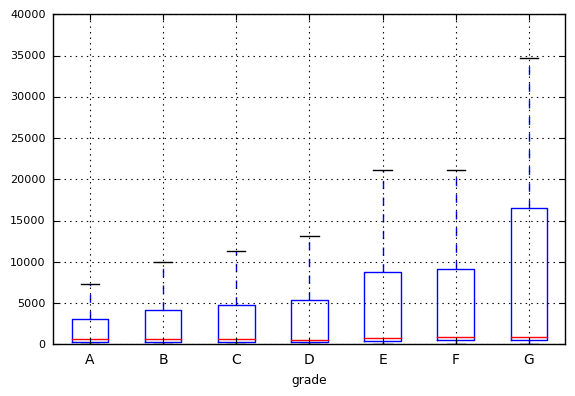
\includegraphics[width=1.05\textwidth]{img/last_pymnt_amnt_by_grade}}

        \end{subfigure}
\\
                \caption{\emph{Boxplots} de total\textunderscore rec\textunderscore prncp }
        \begin{subfigure}[t]{0.45\textwidth}
            \centering

            \centerline{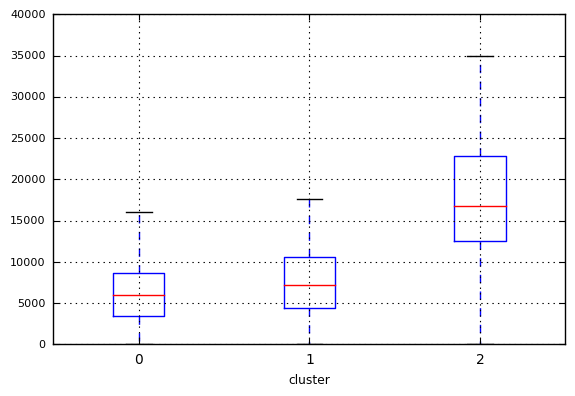
\includegraphics[width=1.05\textwidth]{img/total_rec_prncp_by_cluster}}
        \end{subfigure}%
        ~ 
        \begin{subfigure}[t]{0.45\textwidth}
            \centering
   
            \centerline{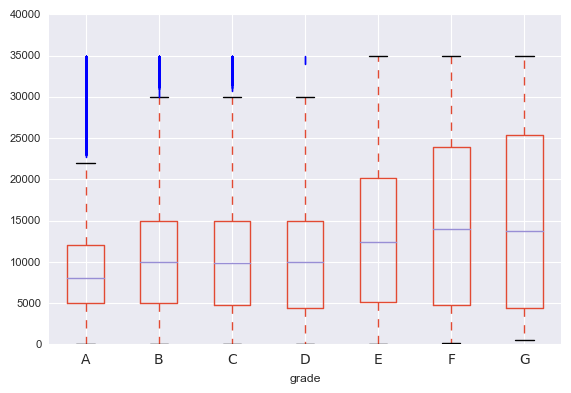
\includegraphics[width=1.05\textwidth]{img/total_rec_prncp_by_grade}}

        \end{subfigure}
\end{figure*}



\begin{figure*}[t!]
    \centering
        \caption{\emph{Boxplots} de total\textunderscore rec\textunderscore late\textunderscore fee }
        \begin{subfigure}[t]{0.45\textwidth}
            \centering

            \centerline{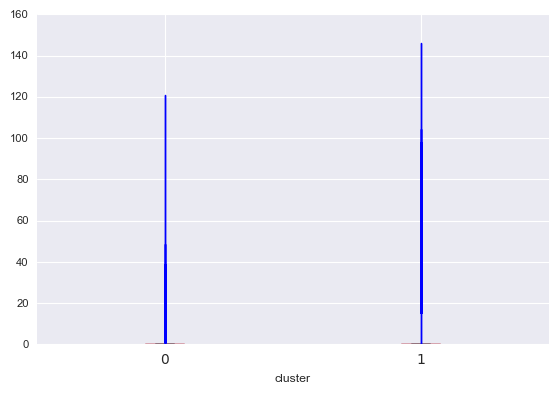
\includegraphics[width=1\textwidth]{img/total_rec_late_fee_by_cluster}}
        \end{subfigure}%
        ~ 
        \begin{subfigure}[t]{0.45\textwidth}
            \centering
   
            \centerline{\includegraphics[width=1\textwidth]{img/total_rec_late_fee_by_grade}}

        \end{subfigure}
                \\
                \caption{\emph{Boxplots} de dti}
        \begin{subfigure}[t]{0.45\textwidth}
            \centering

            \centerline{\includegraphics[width=1.05\textwidth]{img/dti_by_cluster}}
        \end{subfigure}%
        ~ 
        \begin{subfigure}[t]{0.45\textwidth}
            \centering
   
            \centerline{\includegraphics[width=1.05\textwidth]{img/dti_by_grade}}

        \end{subfigure}
\end{figure*}

\chapter{Correlacao entre variaveis}


\begin{landscape}

\begin{table}[]


\centering
\caption{Correla\c c\~ao entre vari\'aveis}
\label{my-label}

\scriptsize
\setlength{\tabcolsep}{1.5pt}
\begin{tabular}{lrrrrrrrrrrrrrrrrrrrrrrrrr}
    & 0      & 1      & 2      & 3      & 4      & 5      & 6      & 7      & 8      & 9      & 10     & 11     & 12     & 13     & 14     & 15     & 16     & 17     & 18     & 19     & 20     & 21     & 22     & 23     \\
0  & 1.000  & 0.999  & 0.993  & 0.487  & 0.326  & 0.956  & 0.373  & 0.033  & -0.037 & 0.025  & 0.164  & -0.065 & 0.337  & 0.259  & 0.325  & 0.325  & 0.900  & 0.899  & 0.839  & 0.738  & 0.068  & 0.169  & 0.130  & 0.440  \\
1  & 0.999  & 1.000  & 0.992  & 0.484  & 0.326  & 0.957  & 0.372  & 0.032  & -0.036 & 0.026  & 0.164  & -0.066 & 0.335  & 0.258  & 0.324  & 0.324  & 0.900  & 0.900  & 0.840  & 0.739  & 0.068  & 0.168  & 0.129  & 0.439  \\
2  & 0.993  & 0.992  & 1.000  & 0.498  & 0.333  & 0.946  & 0.373  & 0.034  & -0.036 & 0.022  & 0.165  & -0.064 & 0.338  & 0.262  & 0.328  & 0.328  & 0.893  & 0.892  & 0.831  & 0.737  & 0.068  & 0.168  & 0.129  & 0.439  \\
3  & 0.487  & 0.484  & 0.498  & 1.000  & 0.552  & 0.264  & 0.104  & 0.074  & 0.012  & 0.053  & 0.080  & -0.007 & 0.144  & 0.134  & 0.421  & 0.421  & 0.429  & 0.426  & 0.281  & 0.614  & 0.048  & 0.153  & 0.122  & 0.267  \\
4  & 0.326  & 0.326  & 0.333  & 0.552  & 1.000  & 0.291  & 0.095  & 0.098  & 0.149  & 0.188  & 0.054  & 0.082  & 0.121  & -0.002 & 0.233  & 0.233  & 0.305  & 0.305  & 0.145  & 0.554  & 0.095  & 0.154  & 0.124  & 0.168  \\
5  & 0.956  & 0.957  & 0.946  & 0.264  & 0.291  & 1.000  & 0.387  & 0.022  & -0.027 & 0.030  & 0.164  & -0.060 & 0.334  & 0.241  & 0.219  & 0.219  & 0.866  & 0.867  & 0.836  & 0.648  & 0.072  & 0.144  & 0.110  & 0.399  \\
6  & 0.373  & 0.372  & 0.373  & 0.104  & 0.095  & 0.387  & 1.000  & -0.185 & 0.035  & 0.046  & 0.199  & -0.029 & 0.367  & 0.310  & 0.094  & 0.094  & 0.367  & 0.367  & 0.365  & 0.259  & 0.034  & 0.029  & 0.032  & 0.200  \\
7  & 0.033  & 0.032  & 0.034  & 0.074  & 0.098  & 0.022  & -0.185 & 1.000  & -0.049 & 0.023  & 0.280  & -0.017 & 0.221  & 0.224  & 0.049  & 0.049  & 0.029  & 0.029  & -0.001 & 0.083  & 0.005  & 0.032  & 0.030  & -0.015 \\
8  & -0.037 & -0.036 & -0.036 & 0.012  & 0.149  & -0.027 & 0.035  & -0.049 & 1.000  & -0.006 & 0.007  & 0.003  & -0.066 & 0.069  & 0.014  & 0.014  & -0.026 & -0.026 & -0.048 & 0.031  & 0.036  & 0.012  & 0.015  & -0.010 \\
9  & 0.025  & 0.026  & 0.022  & 0.053  & 0.188  & 0.030  & 0.046  & 0.023  & -0.006 & 1.000  & 0.097  & 0.030  & -0.018 & 0.116  & -0.016 & -0.015 & 0.014  & 0.016  & -0.002 & 0.042  & 0.013  & 0.022  & 0.029  & 0.057  \\
10 & 0.164  & 0.164  & 0.165  & 0.080  & 0.054  & 0.164  & 0.199  & 0.280  & 0.007  & 0.097  & 1.000  & -0.006 & 0.279  & 0.674  & 0.046  & 0.046  & 0.158  & 0.158  & 0.149  & 0.126  & 0.008  & 0.038  & 0.031  & 0.080  \\
11 & -0.065 & -0.066 & -0.064 & -0.007 & 0.082  & -0.060 & -0.029 & -0.017 & 0.003  & 0.030  & -0.006 & 1.000  & -0.077 & -0.027 & -0.023 & -0.023 & -0.060 & -0.061 & -0.069 & -0.018 & -0.009 & -0.011 & -0.014 & -0.023 \\
12 & 0.337  & 0.335  & 0.338  & 0.144  & 0.121  & 0.334  & 0.367  & 0.221  & -0.066 & -0.018 & 0.279  & -0.077 & 1.000  & 0.314  & 0.130  & 0.130  & 0.326  & 0.325  & 0.302  & 0.272  & 0.016  & 0.059  & 0.053  & 0.140  \\
13 & 0.259  & 0.258  & 0.262  & 0.134  & -0.002 & 0.241  & 0.310  & 0.224  & 0.069  & 0.116  & 0.674  & -0.027 & 0.314  & 1.000  & 0.062  & 0.062  & 0.237  & 0.237  & 0.236  & 0.160  & -0.005 & 0.045  & 0.047  & 0.164  \\
14 & 0.325  & 0.324  & 0.328  & 0.421  & 0.233  & 0.219  & 0.094  & 0.049  & 0.014  & -0.016 & 0.046  & -0.023 & 0.130  & 0.062  & 1.000  & 1.000  & 0.363  & 0.361  & 0.218  & 0.612  & 0.036  & -0.047 & -0.034 & -0.153 \\
15 & 0.325  & 0.324  & 0.328  & 0.421  & 0.233  & 0.219  & 0.094  & 0.049  & 0.014  & -0.015 & 0.046  & -0.023 & 0.130  & 0.062  & 1.000  & 1.000  & 0.363  & 0.361  & 0.218  & 0.612  & 0.036  & -0.047 & -0.034 & -0.153 \\
16 & 0.900  & 0.900  & 0.893  & 0.429  & 0.305  & 0.866  & 0.367  & 0.029  & -0.026 & 0.014  & 0.158  & -0.060 & 0.326  & 0.237  & 0.363  & 0.363  & 1.000  & 1.000  & 0.957  & 0.803  & 0.029  & 0.030  & 0.038  & 0.504  \\
17 & 0.899  & 0.900  & 0.892  & 0.426  & 0.305  & 0.867  & 0.367  & 0.029  & -0.026 & 0.016  & 0.158  & -0.061 & 0.325  & 0.237  & 0.361  & 0.361  & 1.000  & 1.000  & 0.958  & 0.802  & 0.029  & 0.029  & 0.037  & 0.503  \\
18 & 0.839  & 0.840  & 0.831  & 0.281  & 0.145  & 0.836  & 0.365  & -0.001 & -0.048 & -0.002 & 0.149  & -0.069 & 0.302  & 0.236  & 0.218  & 0.218  & 0.957  & 0.958  & 1.000  & 0.611  & -0.016 & -0.113 & -0.078 & 0.594  \\
19 & 0.738  & 0.739  & 0.737  & 0.614  & 0.554  & 0.648  & 0.259  & 0.083  & 0.031  & 0.042  & 0.126  & -0.018 & 0.272  & 0.160  & 0.612  & 0.612  & 0.803  & 0.802  & 0.611  & 1.000  & 0.108  & 0.096  & 0.088  & 0.168  \\
20 & 0.068  & 0.068  & 0.068  & 0.048  & 0.095  & 0.072  & 0.034  & 0.005  & 0.036  & 0.013  & 0.008  & -0.009 & 0.016  & -0.005 & 0.036  & 0.036  & 0.029  & 0.029  & -0.016 & 0.108  & 1.000  & 0.065  & 0.058  & -0.067 \\
21 & 0.169  & 0.168  & 0.168  & 0.153  & 0.154  & 0.144  & 0.029  & 0.032  & 0.012  & 0.022  & 0.038  & -0.011 & 0.059  & 0.045  & -0.047 & -0.047 & 0.030  & 0.029  & -0.113 & 0.096  & 0.065  & 1.000  & 0.797  & -0.083 \\
22 & 0.130  & 0.129  & 0.129  & 0.122  & 0.124  & 0.110  & 0.032  & 0.030  & 0.015  & 0.029  & 0.031  & -0.014 & 0.053  & 0.047  & -0.034 & -0.034 & 0.038  & 0.037  & -0.078 & 0.088  & 0.058  & 0.797  & 1.000  & -0.060 \\
23 & 0.440  & 0.439  & 0.439  & 0.267  & 0.168  & 0.399  & 0.200  & -0.015 & -0.010 & 0.057  & 0.080  & -0.023 & 0.140  & 0.164  & -0.153 & -0.153 & 0.504  & 0.503  & 0.594  & 0.168  & -0.067 & -0.083 & -0.060 & 1.000 
\end{tabular}
\end{table}

\end{landscape}

\chapter{\emph{Silhoutte score}}


É possível fazer uma análise para verificar a quantidade de \emph{clusters} ideal para a amostragem. A cada execução do algoritmo também calcula-se um \emph{score} chamado \emph{sillhouette}, que é uma forma de interpretar e mensurar a validação da consistência dos \emph{clusters}, além de fornecer uma representação gráfica de quão bem os dados estão inseridos nos \emph{clusters} (coesão) em comparação a outros (separação). Esse \emph{score} varia de -1 a 1, na qual quanto mais próximo de 1, mais bem encaixado encontra-se o elemento com seu respectivo \emph{cluster}.

\begin{figure}[!ht]
\caption{An\'alise de 2 \emph{clusters} }
\centerline{\includegraphics[width=.85\textwidth]{img/silhoute2}}
\fonte{Gerado a partir do script}
\end{figure}

\begin{figure}[!ht]
\caption{An\'alise de 3 \emph{clusters} }
\centerline{\includegraphics[width=.85\textwidth]{img/silhoute3}}
\fonte{Gerado a partir do script}
\end{figure}


\begin{figure}[!ht]
\caption{An\'alise de 4 \emph{clusters} }
\centerline{\includegraphics[width=.85\textwidth]{img/silhoute4}}
\fonte{Gerado a partir do script}
\end{figure}

A princípio o \emph{silhoutte score} seria uma métrica de avaliação para definir a quantidade ideal de \emph{clusters} para a execução do K Médias. Contudo, essa métrica não foi implementada no \emph{Apache Spark}, sendo útil apenas para uma análise exploratória.

A primeira tentativa foi de separar a amostra em 2 \emph{clusters}. Para essa divisão, foi obtida uma de 0,6428. Para a divisão em 3 \emph{clusters}, foi obtida 0,6188. Já para 4 \emph{clusters}, 0,6099.


\chapter{Diagrama de Voronoi}

O diagrama de Voronoi é uma ferramenta utilizada para visualizar problemas que envolvem conceito de proximidade em um plano. Baseia-se no fato de que em um plano, existem pontos que estão mais próximos de uma fonte geradora do que de outra fonte, o resultado é um polígono de cujas distâncias entre a fonte e ponto são as menores possíveis. Portanto, é possível ter uma visualização espacial da distribuição dos registros, bem como os centróides.

\begin{figure}[!ht]
\caption{Visualização dos pontos no diagrama de Voronoi com os dados sem normaliza\c c\~ao}
\centerline{\includegraphics[width=0.5\textwidth]{img/voronoi}}
\fonte{Gerado a partir do script}
\end{figure}

A imagem mostra um diagrama de Voronoi. Os polígonos externos se estendem infinitamente no plano, logo são desenhados como figuras abertas. Cada aresta do diagrama constitui um lugar onde os pontos são equidistantes em relação a dois locais. Os vértices dos polígonos estão ligados outras arestas sendo pontos de equidistânciacada região definidas.

Para a visualização desse diagrama, foi necessário realizar uma operação de redução de dimensionalidade de variáveis para 2 \emph{features}. Neste estudo, aplicamos a construção do diagrama para 8000 registros. Embora a redução de dimensionalidade possa distorcer os dados, é possível ter uma visualização de como os dados estão distribuídos num espaço bidimensional. No contexto de \emph{Big Data}, a geração de Diagrama de Voronoi pode ajudar numa análise inicial, sendo inviável gerá-lo para uma base completa e com muitos dados.

% ---
%\chapter{Morbi ultrices rutrum lorem.}
% ---
%\lipsum[30]

% ---
%\chapter{Cras non urna sed feugiat cum sociis natoque penatibus et magnis dis
%parturient montes nascetur ridiculus mus}
% ---

%\lipsum[31]

% ---
%\chapter{Fusce facilisis lacinia dui}
% ---

%\lipsum[32]

\end{anexosenv}

%% ----------------------------------------------------------
% Anexos
% ----------------------------------------------------------

% ---
% Inicia os anexos
% ---
\begin{anexosenv}

% Imprime uma página indicando o início dos anexos
\partanexos


\chapter{Tabela de dados}

Para o caso do \emph{Loan Club}, nem todas as variáveis foram utilizadas. Isto se deve ao fato de que algumas das variáveis em questão são categóricas, outras que representam alguma descrição. Tratam-se de campos que provem informações substanciais mais que para o escopo deste trabalho foram desconsideradas. No caso de variáveis categóricas, seria possível uma conversão para variáveis \emph{dummies}, mas que para o caso do K Médias não devem ser consideradas. Já para os campos que possuem uma informação textual, existem algoritmos que podem fazer análises do conteúdo como \emph{word to vec} ou \emph{bag of words}.

 \label{tab:daypack}
    \begin{tabularx}{\textwidth}{p{.3\textwidth}X}
    \caption{Tabela de campos utilizados para a an\'alise do banco de dados \emph{Loan Club}}\\
    \toprule
    \textbf{Coluna} & \textbf{Descrição} \\[6pt]
    \midrule
    \endhead

funded\textunderscore amnt & Total do montante comprometido para aquele empr\'estimo at\'e este momento\\
funded\textunderscore amnt\textunderscore inv & Total do montante comprometido pelos investidores para aquele empr\'estimo at\'e este momento\\
grade & Nota atribu\'ida pelo \emph{Loan Club}\\
loan\textunderscore amnt & A quantia do empr\'estimo do mutu\'ario, podendo ter eventualmente descontos pelo departamento de cr\'edito\\
term & Quantidade de pagamentos do empr\'estimos que pode ser de 36 ou 60 meses\\
int\textunderscore rate & Taxa de juros do empr\'estimo\\
installment & Pagamento devido pelo tomador de empr\'estimo\\
annual\textunderscore inc & Renda anual relatada pelo devedor durante o cadastro\\
dti\textunderscore joint & A raz\~ao entre a quantia total de d\'ividas paga pelos co-mutu\'arios (desconsiderando hipotecas e o empr\'estimo feito pelo \emph{Loan Club}) dividido pela renda mensal dos co-mutu\'arios\\
delinq\textunderscore 2yrs & Incid\^encias de inadimpl\^encia (eventos ocorridos dentro de 30 dias) dentro de um per\'iodo de 2 anos\\
inq\textunderscore last\textunderscore 6mths & Quantidade de pedidos de empr\'estimos (excluindo carros e hipotecas)\\
open\textunderscore acc & N\'umero de linhas de cr\'editos abertas para o mutu\'ario\\
pub\textunderscore rec & N\'umero de \"derogatory public records\" (trata-se de um registro que pode ser considerado negativo para o mutu\'ario pois indica um risco e denegrindo sua reputa\c c\~ao e dificultando a possibilidade de aquisi\c c\~ao de outros produtos. Entre os valores, \'e poss\'ivel W e F\\
revol\textunderscore bal & Total de cr\'edito que n\~ao foi pago\\
total\textunderscore acc & N\'umero toral de linhas de cr\'editos usada pelo mutu\'ario\\
out\textunderscore prncp & Saldo devedor\\
out\textunderscore prncp\textunderscore inv & Saldo devedor sobre a por\c c\~ao de capital financiado por investidores\\
total\textunderscore pymnt & Pagamentos recebidos at\'e o momento presente sobre o valor financiado\\
total\textunderscore pymnt\textunderscore inv & Pagamentos recebidos at\'e o momento presente sobre o valor financiado pelo investidor\\
total\textunderscore rec\textunderscore int & Juros recebido at\'e a data presente\\
total\textunderscore rec\textunderscore late\textunderscore fee & Taxas de atraso recebido at\'e a presente data\\
total\textunderscore rec\textunderscore prncp & Capital financiado recebido at\'e a data presente\\
collection\textunderscore recovery\textunderscore fee & valor de imposto recuperado de \"charge off\" (declara\c c\~ao de n\~ao quita\c c\~ao de uma d\'ivida)\\
last\textunderscore pymnt\textunderscore amnt & Valor total de pagamento recebido\\
recoveries & valor bruto recuperado de \"charge off\" verificados \\
\bottomrule

\end{tabularx}


 \label{tab:daypack}
    \begin{tabularx}{\textwidth}{p{.3\textwidth}X}
    \caption{Tabela de campos disponíveis em \emph{Loan Club} e que n\~ao foram utilizados}\\
    \toprule
    \textbf{Coluna} & \textbf{Descrição} \\[6pt]
    \midrule
    \endhead

addr\textunderscore state & Estado de moradia do mutu\'ario\\
annual\textunderscore inc\textunderscore joint & Valor declarado no momento do cadastro da renda anual do co-mutu\'arios (um emprestimo eh realizado com co-mutuarios quando mais de uma pessao eh sao financiadas)\\
application\textunderscore type & Indica se o empr\'estimo ser\'a individual ou se ser\'a feito por mais de uma pessoa (co-mutu\'arios) \\
earliest\textunderscore cr\textunderscore line & M\^es mais recente em que o mutu\'ario abriu uma linha de cr\'edito\\
emp\textunderscore length & Per\'iodo em que o devedor est\'a empregado no trabalho atual, na qual 0 representa menos de 1 ano e 10 pode ser de 10 a mais anos \\
emp\textunderscore title & Descri\c c\~ao breve do emprego do devedor\\
fico\textunderscore range\textunderscore high & Limite superior do score proveniente do FICO a qual o devedor est\'a enquadrado\\
fico\textunderscore range\textunderscore low & Limite inferior do score proveniente do FICO a qual o devedor est\'a enquadrado\\
home\textunderscore ownership & Indica o status do tipo de moradia do tomador de empr\'estimo RENT (aluguel), OWN (casa pr\'opria), MORTGAGE (hipoteca), OTHER (outros)\\
id & vari\'avel de identifica\c c\~ao de cada cliente da \emph{Loan Club}\\
initial\textunderscore list\textunderscore status & Status inicial e interno da \emph{Loan Club} do mutu\'ario. Varia entre W e F\\
is\textunderscore inc\textunderscore v & Indica se a renda foi verificada pela \emph{Loan Club} ou n\~ao ou se a fonte de renda foi verificada\\
issue\textunderscore d & M\^es no qual o empr\'estimo foi financiado\\
last\textunderscore credit\textunderscore pull\textunderscore d & O m\^es mais recente desde que o mutu\'ario adquiriu cr\'edito no financiamento\\
last\textunderscore fico\textunderscore range\textunderscore high & O limite superior do \'ultimo score do FICO em que o mutu\'ario foi classificado\\
last\textunderscore fico\textunderscore range\textunderscore low & O limite inferior do \'ultimo score do FICO em que o mutu\'ario foi classificado\\
last\textunderscore pymnt\textunderscore d & \'Ultimo m\^es em que foi recebido um pagamento\\
loan\textunderscore status & Status atual do empr\'estimo\\
mths\textunderscore since\textunderscore last\textunderscore delinq & N\'umero de meses desde a \'ultima inadimpl\^encia do mutu\'ario\\
mths\textunderscore since\textunderscore last\textunderscore major\textunderscore derog & Meses desde a pior nota (em um per\'iodo de 90 dias)\\
mths\textunderscore since\textunderscore last\textunderscore record & N\'unmero de meses desde o \'ultimo registro de informa\c c\~oes p\'ublicas (anteced\^encia criminal)\\
next\textunderscore pymnt\textunderscore d & Data do pr\'oximo pagamento\\
policy\textunderscore code & C\'odigo interno da \emph{Loan Club}, variando entre 1 e 2\\
purpose & Categoria escolhida pelo mutu\'ario no momento da solicita\c c\~ao do cr\'edito\\
pymnt\textunderscore plan & Indica se o pagamento do plano est\'a em dia\\
revol\textunderscore util & Taxa de utiliza\c c\~ao da linha de cr\'edito (revolving account)\\
sub\textunderscore grade & Sub nota atribu\'ida pelo Loan Club\\
title & Tipo de empr\'estimo realizado pelo mutu\'ario\\
verified\textunderscore status\textunderscore joint & Indica se a renda dos co-mutu\'arios foi verificada pela \emph{Loan Club}, se n\~ao foi ou se a fonte de renda foi verificada\\
zip\textunderscore code & Os primeiros 3 n\'umeros de c\'odigo postal fornecida pelo mutu\'ario\\
open\textunderscore acc\textunderscore 6m & N\'umero de neg\'ocios abertos nos \'ultimos 6 meses\\
open\textunderscore il\textunderscore 6m & N\'umero de opera\c c\~oes de financiamento ativos \\
open\textunderscore il\textunderscore 12m & N\'umero de contas de opera\c c\~oes de financiamento abertas nos \'ultimos 12 meses\\
open\textunderscore il\textunderscore 24m & N\'umero de contas de opera\c c\~oes de financiamento abertas nos \'ultimos 24 meses\\
mths\textunderscore since\textunderscore rcnt\textunderscore il & Quantidade de meses desde que a mais recente conta de opera\c c\~oes de financiamento aberta\\
total\textunderscore bal\textunderscore il & Saldo total de todas as installment accounts\\
il\textunderscore util & Raz\~ao entre o total de saldo sobre o limite de cr\'edito para todas as installment accounts\\
open\textunderscore rv\textunderscore 12m & Quantidade de contas (revolving accounts) nos \'ultimos 12 meses\\
open\textunderscore rv\textunderscore 24m & Quantidade de contas (revolving accounts) abertas nos \'ultimos 24 meses\\
max\textunderscore bal\textunderscore bc & Saldo atual de todas as contas abertas (revolving accounts)\\
all\textunderscore util & Saldo de limite de cr\'editos para todas as opera\c c\~oes\\
total\textunderscore rev\textunderscore hi\textunderscore lim & Total limite de revolving cr\'editos\\
inq\textunderscore fi & N\'umero de solicita\c c\~oes de cr\'edito para finan\c cas pessoais\\
total\textunderscore cu\textunderscore tl & N\'umero de neg\'ocios financeiros\\

acc\textunderscore now\textunderscore delinq & N\'umero de contas nas quais o mutu\'ario est\'a agora inadimplente\\
tot\textunderscore coll\textunderscore amt & Saldo total de collection accounts \\
tot\textunderscore cur\textunderscore bal & Saldo total de todas as contas do mutuário \\
\bottomrule

\end{tabularx}


\chapter{Análise dos \emph{clusters} vs \emph{grades}}

Durante os estudos, foram feitas algumas análises com \emph{boxplots} para entender os \emph{clusters} gerados. Também foram feitos uma comparação com os clientes de acordo com os seus grades para ver se era possível encontrar algum padrão nos registros. Detectar padrões de dados é uma tarefa complexa e visto que não se trata do foco do trabalho, o estudo limitou-se a verificar apenas alguma ocorrência de padrão.

Nos anexos, estão os outros \emph{boxplots} gerados que não constam na parte de Resultados.

\clearpage

\begin{figure*}[t!]
    \centering
        \caption{\emph{Boxplots} de collection\textunderscore recovery\textunderscore fee }
        \begin{subfigure}[t]{0.45\textwidth}
            \centering
            \caption{Cluster }

            \centerline{\includegraphics[width=1\textwidth]{img/collection_recovery_fee_by_cluster}}
        \end{subfigure}%
        ~ 
        \begin{subfigure}[t]{0.45\textwidth}
            \centering
            \caption{Grade}
   
            \centerline{\includegraphics[width=1\textwidth]{img/collection_recovery_fee_by_grade}}

        \end{subfigure}
        \\
                \caption{\emph{Boxplots} de funded\textunderscore amnt}
        \begin{subfigure}[t]{0.45\textwidth}
            \centering

            \centerline{\includegraphics[width=1.05\textwidth]{img/funded_amnt_by_cluster}}
        \end{subfigure}%
        ~ 
        \begin{subfigure}[t]{0.45\textwidth}
            \centering
   
            \centerline{\includegraphics[width=1.05\textwidth]{img/funded_amnt_by_grade}}

        \end{subfigure}

\end{figure*}

\begin{figure*}[t!]
    \centering
        \caption{\emph{Boxplots} de funded\textunderscore amnt\textunderscore inv }
        \begin{subfigure}[t]{0.45\textwidth}
 
            \centerline{\includegraphics[width=1\textwidth]{img/funded_amnt_inv_by_cluster}}
        \end{subfigure}%
        ~ 
        \begin{subfigure}[t]{0.45\textwidth}
            \centerline{\includegraphics[width=1\textwidth]{img/funded_amnt_inv_by_grade}}

        \end{subfigure}
        \\
                \caption{\emph{Boxplots} de installment}
        \begin{subfigure}[t]{0.45\textwidth}
            \centering

            \centerline{\includegraphics[width=1.05\textwidth]{img/installment_by_cluster}}
        \end{subfigure}%
        ~ 
        \begin{subfigure}[t]{0.45\textwidth}
            \centering
   
            \centerline{\includegraphics[width=1.05\textwidth]{img/installment_by_grade}}

        \end{subfigure}



\end{figure*}

\begin{figure*}[t!]
    \centering
        \caption{\emph{Boxplots} de term\textunderscore float\textunderscore fee }
        \begin{subfigure}[t]{0.45\textwidth}
            \centering

            \centerline{\includegraphics[width=1\textwidth]{img/term_float_by_cluster}}
        \end{subfigure}%
        ~ 
        \begin{subfigure}[t]{0.45\textwidth}
            \centering
   
            \centerline{\includegraphics[width=1\textwidth]{img/term_float_by_grade}}

        \end{subfigure}
        \\
                \caption{\emph{Boxplots} de loan\textunderscore amnt}
        \begin{subfigure}[t]{0.45\textwidth}
            \centering

            \centerline{\includegraphics[width=1.05\textwidth]{img/loan_amnt_by_cluster}}
        \end{subfigure}%
        ~ 
        \begin{subfigure}[t]{0.45\textwidth}
            \centering
   
            \centerline{\includegraphics[width=1.05\textwidth]{img/loan_amnt_by_grade}}

        \end{subfigure}
\\
                \caption{\emph{Boxplots} de int\textunderscore rate\textunderscore float}
        \begin{subfigure}[t]{0.45\textwidth}
            \centering

            \centerline{\includegraphics[width=1.05\textwidth]{img/int_rate_float_by_cluster}}
        \end{subfigure}%
        ~ 
        \begin{subfigure}[t]{0.45\textwidth}
            \centering
   
            \centerline{\includegraphics[width=1.05\textwidth]{img/int_rate_float_by_grade}}

        \end{subfigure}
\end{figure*}



\begin{figure*}[t!]
    \centering
        \caption{\emph{Boxplots} de annual\textunderscore inc }
        \begin{subfigure}[t]{0.45\textwidth}
            \centering

            \centerline{\includegraphics[width=1\textwidth]{img/annual_inc_by_cluster}}
        \end{subfigure}%
        ~ 
        \begin{subfigure}[t]{0.45\textwidth}
            \centering
   
            \centerline{\includegraphics[width=1\textwidth]{img/annual_inc_by_grade}}

        \end{subfigure}
        \\
                \caption{\emph{Boxplots} de delinq\textunderscore 2yrs}
        \begin{subfigure}[t]{0.45\textwidth}
            \centering

            \centerline{\includegraphics[width=1.05\textwidth]{img/delinq_2yrs_by_cluster}}
        \end{subfigure}%
        ~ 
        \begin{subfigure}[t]{0.45\textwidth}
            \centering
   
            \centerline{\includegraphics[width=1.05\textwidth]{img/delinq_2yrs_by_grade}}

        \end{subfigure}
\\
                \caption{\emph{Boxplots} de recoveries}
        \begin{subfigure}[t]{0.45\textwidth}
            \centering

            \centerline{\includegraphics[width=1.05\textwidth]{img/recoveries_by_cluster}}
        \end{subfigure}%
        ~ 
        \begin{subfigure}[t]{0.45\textwidth}
            \centering
   
            \centerline{\includegraphics[width=1.05\textwidth]{img/recoveries_by_grade}}

        \end{subfigure}
\end{figure*}


\begin{figure*}[t!]
    \centering
        \caption{\emph{Boxplots} de open\textunderscore acc }
        \begin{subfigure}[t]{0.45\textwidth}
            \centering

            \centerline{\includegraphics[width=1\textwidth]{img/open_acc_by_cluster}}
        \end{subfigure}%
        ~ 
        \begin{subfigure}[t]{0.45\textwidth}
            \centering
   
            \centerline{\includegraphics[width=1\textwidth]{img/open_acc_by_grade}}

        \end{subfigure}
        \\
                \caption{\emph{Boxplots} de pub\textunderscore rec}
        \begin{subfigure}[t]{0.45\textwidth}
            \centering

            \centerline{\includegraphics[width=1.05\textwidth]{img/pub_rec_by_cluster}}
        \end{subfigure}%
        ~ 
        \begin{subfigure}[t]{0.45\textwidth}
            \centering
   
            \centerline{\includegraphics[width=1.05\textwidth]{img/pub_rec_by_grade}}

        \end{subfigure}
\\
                \caption{\emph{Boxplots} de inq\textunderscore last\textunderscore 6mths}
        \begin{subfigure}[t]{0.45\textwidth}
            \centering

            \centerline{\includegraphics[width=1.05\textwidth]{img/inq_last_6mths_by_cluster}}
        \end{subfigure}%
        ~ 
        \begin{subfigure}[t]{0.45\textwidth}
            \centering
   
            \centerline{\includegraphics[width=1.05\textwidth]{img/inq_last_6mths_by_grade}}

        \end{subfigure}
\end{figure*}

\begin{figure*}[t!]
    \centering
        \caption{\emph{Boxplots} de revol\textunderscore bal }
        \begin{subfigure}[t]{0.45\textwidth}
            \centering

            \centerline{\includegraphics[width=1\textwidth]{img/revol_bal_by_cluster}}
        \end{subfigure}%
        ~ 
        \begin{subfigure}[t]{0.45\textwidth}
            \centering
   
            \centerline{\includegraphics[width=1\textwidth]{img/revol_bal_by_grade}}

        \end{subfigure}
        \\
                \caption{\emph{Boxplots} de total\textunderscore acc}
        \begin{subfigure}[t]{0.45\textwidth}
            \centering

            \centerline{\includegraphics[width=1.05\textwidth]{img/total_acc_by_cluster}}
        \end{subfigure}%
        ~ 
        \begin{subfigure}[t]{0.45\textwidth}
            \centering
   
            \centerline{\includegraphics[width=1.05\textwidth]{img/total_acc_by_grade}}

        \end{subfigure}
\\
                \caption{\emph{Boxplots} de out\textunderscore prncp}
        \begin{subfigure}[t]{0.45\textwidth}
            \centering

            \centerline{\includegraphics[width=1.05\textwidth]{img/out_prncp_by_cluster}}
        \end{subfigure}%
        ~ 
        \begin{subfigure}[t]{0.45\textwidth}
            \centering
   
            \centerline{\includegraphics[width=1.05\textwidth]{img/out_prncp_by_grade}}

        \end{subfigure}
\end{figure*}


\begin{figure*}[t!]
    \centering
        \caption{\emph{Boxplots} de total\textunderscore pymnt }
        \begin{subfigure}[t]{0.45\textwidth}
            \centering

            \centerline{\includegraphics[width=1\textwidth]{img/total_pymnt_by_cluster}}
        \end{subfigure}%
        ~ 
        \begin{subfigure}[t]{0.45\textwidth}
            \centering
   
            \centerline{\includegraphics[width=1\textwidth]{img/total_pymnt_by_grade}}

        \end{subfigure}
        \\
                \caption{\emph{Boxplots} de out\textunderscore prncp\textunderscore inv}
        \begin{subfigure}[t]{0.45\textwidth}
            \centering

            \centerline{\includegraphics[width=1.05\textwidth]{img/out_prncp_inv_by_cluster}}
        \end{subfigure}%
        ~ 
        \begin{subfigure}[t]{0.45\textwidth}
            \centering
   
            \centerline{\includegraphics[width=1.05\textwidth]{img/out_prncp_inv_by_grade}}

        \end{subfigure}
\\
                \caption{\emph{Boxplots} de total\textunderscore rec\textunderscore int }
        \begin{subfigure}[t]{0.45\textwidth}
            \centering

            \centerline{\includegraphics[width=1.05\textwidth]{img/total_rec_int_by_cluster}}
        \end{subfigure}%
        ~ 
        \begin{subfigure}[t]{0.45\textwidth}
            \centering
   
            \centerline{\includegraphics[width=1.05\textwidth]{img/total_rec_int_by_grade}}

        \end{subfigure}
\end{figure*}



\begin{figure*}[t!]
    \centering
        \caption{\emph{Boxplots} de total\textunderscore pymnt\textunderscore inv }
        \begin{subfigure}[t]{0.45\textwidth}
            \centering

            \centerline{\includegraphics[width=1\textwidth]{img/total_pymnt_inv_by_cluster}}
        \end{subfigure}%
        ~ 
        \begin{subfigure}[t]{0.45\textwidth}
            \centering
   
            \centerline{\includegraphics[width=1\textwidth]{img/total_pymnt_inv_by_grade}}

        \end{subfigure}
        \\
                \caption{\emph{Boxplots} de last\textunderscore pymnt\textunderscore amnt}
        \begin{subfigure}[t]{0.45\textwidth}
            \centering

            \centerline{\includegraphics[width=1.05\textwidth]{img/last_pymnt_amnt_by_cluster}}
        \end{subfigure}%
        ~ 
        \begin{subfigure}[t]{0.45\textwidth}
            \centering
   
            \centerline{\includegraphics[width=1.05\textwidth]{img/last_pymnt_amnt_by_grade}}

        \end{subfigure}
\\
                \caption{\emph{Boxplots} de total\textunderscore rec\textunderscore prncp }
        \begin{subfigure}[t]{0.45\textwidth}
            \centering

            \centerline{\includegraphics[width=1.05\textwidth]{img/total_rec_prncp_by_cluster}}
        \end{subfigure}%
        ~ 
        \begin{subfigure}[t]{0.45\textwidth}
            \centering
   
            \centerline{\includegraphics[width=1.05\textwidth]{img/total_rec_prncp_by_grade}}

        \end{subfigure}
\end{figure*}



\begin{figure*}[t!]
    \centering
        \caption{\emph{Boxplots} de total\textunderscore rec\textunderscore late\textunderscore fee }
        \begin{subfigure}[t]{0.45\textwidth}
            \centering

            \centerline{\includegraphics[width=1\textwidth]{img/total_rec_late_fee_by_cluster}}
        \end{subfigure}%
        ~ 
        \begin{subfigure}[t]{0.45\textwidth}
            \centering
   
            \centerline{\includegraphics[width=1\textwidth]{img/total_rec_late_fee_by_grade}}

        \end{subfigure}
                \\
                \caption{\emph{Boxplots} de dti}
        \begin{subfigure}[t]{0.45\textwidth}
            \centering

            \centerline{\includegraphics[width=1.05\textwidth]{img/dti_by_cluster}}
        \end{subfigure}%
        ~ 
        \begin{subfigure}[t]{0.45\textwidth}
            \centering
   
            \centerline{\includegraphics[width=1.05\textwidth]{img/dti_by_grade}}

        \end{subfigure}
\end{figure*}

\chapter{Correlacao entre variaveis}


\begin{landscape}

\begin{table}[]


\centering
\caption{Correla\c c\~ao entre vari\'aveis}
\label{my-label}

\scriptsize
\setlength{\tabcolsep}{1.5pt}
\begin{tabular}{lrrrrrrrrrrrrrrrrrrrrrrrrr}
    & 0      & 1      & 2      & 3      & 4      & 5      & 6      & 7      & 8      & 9      & 10     & 11     & 12     & 13     & 14     & 15     & 16     & 17     & 18     & 19     & 20     & 21     & 22     & 23     \\
0  & 1.000  & 0.999  & 0.993  & 0.487  & 0.326  & 0.956  & 0.373  & 0.033  & -0.037 & 0.025  & 0.164  & -0.065 & 0.337  & 0.259  & 0.325  & 0.325  & 0.900  & 0.899  & 0.839  & 0.738  & 0.068  & 0.169  & 0.130  & 0.440  \\
1  & 0.999  & 1.000  & 0.992  & 0.484  & 0.326  & 0.957  & 0.372  & 0.032  & -0.036 & 0.026  & 0.164  & -0.066 & 0.335  & 0.258  & 0.324  & 0.324  & 0.900  & 0.900  & 0.840  & 0.739  & 0.068  & 0.168  & 0.129  & 0.439  \\
2  & 0.993  & 0.992  & 1.000  & 0.498  & 0.333  & 0.946  & 0.373  & 0.034  & -0.036 & 0.022  & 0.165  & -0.064 & 0.338  & 0.262  & 0.328  & 0.328  & 0.893  & 0.892  & 0.831  & 0.737  & 0.068  & 0.168  & 0.129  & 0.439  \\
3  & 0.487  & 0.484  & 0.498  & 1.000  & 0.552  & 0.264  & 0.104  & 0.074  & 0.012  & 0.053  & 0.080  & -0.007 & 0.144  & 0.134  & 0.421  & 0.421  & 0.429  & 0.426  & 0.281  & 0.614  & 0.048  & 0.153  & 0.122  & 0.267  \\
4  & 0.326  & 0.326  & 0.333  & 0.552  & 1.000  & 0.291  & 0.095  & 0.098  & 0.149  & 0.188  & 0.054  & 0.082  & 0.121  & -0.002 & 0.233  & 0.233  & 0.305  & 0.305  & 0.145  & 0.554  & 0.095  & 0.154  & 0.124  & 0.168  \\
5  & 0.956  & 0.957  & 0.946  & 0.264  & 0.291  & 1.000  & 0.387  & 0.022  & -0.027 & 0.030  & 0.164  & -0.060 & 0.334  & 0.241  & 0.219  & 0.219  & 0.866  & 0.867  & 0.836  & 0.648  & 0.072  & 0.144  & 0.110  & 0.399  \\
6  & 0.373  & 0.372  & 0.373  & 0.104  & 0.095  & 0.387  & 1.000  & -0.185 & 0.035  & 0.046  & 0.199  & -0.029 & 0.367  & 0.310  & 0.094  & 0.094  & 0.367  & 0.367  & 0.365  & 0.259  & 0.034  & 0.029  & 0.032  & 0.200  \\
7  & 0.033  & 0.032  & 0.034  & 0.074  & 0.098  & 0.022  & -0.185 & 1.000  & -0.049 & 0.023  & 0.280  & -0.017 & 0.221  & 0.224  & 0.049  & 0.049  & 0.029  & 0.029  & -0.001 & 0.083  & 0.005  & 0.032  & 0.030  & -0.015 \\
8  & -0.037 & -0.036 & -0.036 & 0.012  & 0.149  & -0.027 & 0.035  & -0.049 & 1.000  & -0.006 & 0.007  & 0.003  & -0.066 & 0.069  & 0.014  & 0.014  & -0.026 & -0.026 & -0.048 & 0.031  & 0.036  & 0.012  & 0.015  & -0.010 \\
9  & 0.025  & 0.026  & 0.022  & 0.053  & 0.188  & 0.030  & 0.046  & 0.023  & -0.006 & 1.000  & 0.097  & 0.030  & -0.018 & 0.116  & -0.016 & -0.015 & 0.014  & 0.016  & -0.002 & 0.042  & 0.013  & 0.022  & 0.029  & 0.057  \\
10 & 0.164  & 0.164  & 0.165  & 0.080  & 0.054  & 0.164  & 0.199  & 0.280  & 0.007  & 0.097  & 1.000  & -0.006 & 0.279  & 0.674  & 0.046  & 0.046  & 0.158  & 0.158  & 0.149  & 0.126  & 0.008  & 0.038  & 0.031  & 0.080  \\
11 & -0.065 & -0.066 & -0.064 & -0.007 & 0.082  & -0.060 & -0.029 & -0.017 & 0.003  & 0.030  & -0.006 & 1.000  & -0.077 & -0.027 & -0.023 & -0.023 & -0.060 & -0.061 & -0.069 & -0.018 & -0.009 & -0.011 & -0.014 & -0.023 \\
12 & 0.337  & 0.335  & 0.338  & 0.144  & 0.121  & 0.334  & 0.367  & 0.221  & -0.066 & -0.018 & 0.279  & -0.077 & 1.000  & 0.314  & 0.130  & 0.130  & 0.326  & 0.325  & 0.302  & 0.272  & 0.016  & 0.059  & 0.053  & 0.140  \\
13 & 0.259  & 0.258  & 0.262  & 0.134  & -0.002 & 0.241  & 0.310  & 0.224  & 0.069  & 0.116  & 0.674  & -0.027 & 0.314  & 1.000  & 0.062  & 0.062  & 0.237  & 0.237  & 0.236  & 0.160  & -0.005 & 0.045  & 0.047  & 0.164  \\
14 & 0.325  & 0.324  & 0.328  & 0.421  & 0.233  & 0.219  & 0.094  & 0.049  & 0.014  & -0.016 & 0.046  & -0.023 & 0.130  & 0.062  & 1.000  & 1.000  & 0.363  & 0.361  & 0.218  & 0.612  & 0.036  & -0.047 & -0.034 & -0.153 \\
15 & 0.325  & 0.324  & 0.328  & 0.421  & 0.233  & 0.219  & 0.094  & 0.049  & 0.014  & -0.015 & 0.046  & -0.023 & 0.130  & 0.062  & 1.000  & 1.000  & 0.363  & 0.361  & 0.218  & 0.612  & 0.036  & -0.047 & -0.034 & -0.153 \\
16 & 0.900  & 0.900  & 0.893  & 0.429  & 0.305  & 0.866  & 0.367  & 0.029  & -0.026 & 0.014  & 0.158  & -0.060 & 0.326  & 0.237  & 0.363  & 0.363  & 1.000  & 1.000  & 0.957  & 0.803  & 0.029  & 0.030  & 0.038  & 0.504  \\
17 & 0.899  & 0.900  & 0.892  & 0.426  & 0.305  & 0.867  & 0.367  & 0.029  & -0.026 & 0.016  & 0.158  & -0.061 & 0.325  & 0.237  & 0.361  & 0.361  & 1.000  & 1.000  & 0.958  & 0.802  & 0.029  & 0.029  & 0.037  & 0.503  \\
18 & 0.839  & 0.840  & 0.831  & 0.281  & 0.145  & 0.836  & 0.365  & -0.001 & -0.048 & -0.002 & 0.149  & -0.069 & 0.302  & 0.236  & 0.218  & 0.218  & 0.957  & 0.958  & 1.000  & 0.611  & -0.016 & -0.113 & -0.078 & 0.594  \\
19 & 0.738  & 0.739  & 0.737  & 0.614  & 0.554  & 0.648  & 0.259  & 0.083  & 0.031  & 0.042  & 0.126  & -0.018 & 0.272  & 0.160  & 0.612  & 0.612  & 0.803  & 0.802  & 0.611  & 1.000  & 0.108  & 0.096  & 0.088  & 0.168  \\
20 & 0.068  & 0.068  & 0.068  & 0.048  & 0.095  & 0.072  & 0.034  & 0.005  & 0.036  & 0.013  & 0.008  & -0.009 & 0.016  & -0.005 & 0.036  & 0.036  & 0.029  & 0.029  & -0.016 & 0.108  & 1.000  & 0.065  & 0.058  & -0.067 \\
21 & 0.169  & 0.168  & 0.168  & 0.153  & 0.154  & 0.144  & 0.029  & 0.032  & 0.012  & 0.022  & 0.038  & -0.011 & 0.059  & 0.045  & -0.047 & -0.047 & 0.030  & 0.029  & -0.113 & 0.096  & 0.065  & 1.000  & 0.797  & -0.083 \\
22 & 0.130  & 0.129  & 0.129  & 0.122  & 0.124  & 0.110  & 0.032  & 0.030  & 0.015  & 0.029  & 0.031  & -0.014 & 0.053  & 0.047  & -0.034 & -0.034 & 0.038  & 0.037  & -0.078 & 0.088  & 0.058  & 0.797  & 1.000  & -0.060 \\
23 & 0.440  & 0.439  & 0.439  & 0.267  & 0.168  & 0.399  & 0.200  & -0.015 & -0.010 & 0.057  & 0.080  & -0.023 & 0.140  & 0.164  & -0.153 & -0.153 & 0.504  & 0.503  & 0.594  & 0.168  & -0.067 & -0.083 & -0.060 & 1.000 
\end{tabular}
\end{table}

\end{landscape}

\chapter{\emph{Silhoutte score}}


É possível fazer uma análise para verificar a quantidade de \emph{clusters} ideal para a amostragem. A cada execução do algoritmo também calcula-se um \emph{score} chamado \emph{sillhouette}, que é uma forma de interpretar e mensurar a validação da consistência dos \emph{clusters}, além de fornecer uma representação gráfica de quão bem os dados estão inseridos nos \emph{clusters} (coesão) em comparação a outros (separação). Esse \emph{score} varia de -1 a 1, na qual quanto mais próximo de 1, mais bem encaixado encontra-se o elemento com seu respectivo \emph{cluster}.

\begin{figure}[!ht]
\caption{An\'alise de 2 \emph{clusters} }
\centerline{\includegraphics[width=.85\textwidth]{img/silhoute2}}
\fonte{Gerado a partir do script}
\end{figure}

\begin{figure}[!ht]
\caption{An\'alise de 3 \emph{clusters} }
\centerline{\includegraphics[width=.85\textwidth]{img/silhoute3}}
\fonte{Gerado a partir do script}
\end{figure}


\begin{figure}[!ht]
\caption{An\'alise de 4 \emph{clusters} }
\centerline{\includegraphics[width=.85\textwidth]{img/silhoute4}}
\fonte{Gerado a partir do script}
\end{figure}

A princípio o \emph{silhoutte score} seria uma métrica de avaliação para definir a quantidade ideal de \emph{clusters} para a execução do K Médias. Contudo, essa métrica não foi implementada no \emph{Apache Spark}, sendo útil apenas para uma análise exploratória.

A primeira tentativa foi de separar a amostra em 2 \emph{clusters}. Para essa divisão, foi obtida uma de 0,6428. Para a divisão em 3 \emph{clusters}, foi obtida 0,6188. Já para 4 \emph{clusters}, 0,6099.


\chapter{Diagrama de Voronoi}

O diagrama de Voronoi é uma ferramenta utilizada para visualizar problemas que envolvem conceito de proximidade em um plano. Baseia-se no fato de que em um plano, existem pontos que estão mais próximos de uma fonte geradora do que de outra fonte, o resultado é um polígono de cujas distâncias entre a fonte e ponto são as menores possíveis. Portanto, é possível ter uma visualização espacial da distribuição dos registros, bem como os centróides.

\begin{figure}[!ht]
\caption{Visualização dos pontos no diagrama de Voronoi com os dados sem normaliza\c c\~ao}
\centerline{\includegraphics[width=0.5\textwidth]{img/voronoi}}
\fonte{Gerado a partir do script}
\end{figure}

A imagem mostra um diagrama de Voronoi. Os polígonos externos se estendem infinitamente no plano, logo são desenhados como figuras abertas. Cada aresta do diagrama constitui um lugar onde os pontos são equidistantes em relação a dois locais. Os vértices dos polígonos estão ligados outras arestas sendo pontos de equidistânciacada região definidas.

Para a visualização desse diagrama, foi necessário realizar uma operação de redução de dimensionalidade de variáveis para 2 \emph{features}. Neste estudo, aplicamos a construção do diagrama para 8000 registros. Embora a redução de dimensionalidade possa distorcer os dados, é possível ter uma visualização de como os dados estão distribuídos num espaço bidimensional. No contexto de \emph{Big Data}, a geração de Diagrama de Voronoi pode ajudar numa análise inicial, sendo inviável gerá-lo para uma base completa e com muitos dados.

% ---
%\chapter{Morbi ultrices rutrum lorem.}
% ---
%\lipsum[30]

% ---
%\chapter{Cras non urna sed feugiat cum sociis natoque penatibus et magnis dis
%parturient montes nascetur ridiculus mus}
% ---

%\lipsum[31]

% ---
%\chapter{Fusce facilisis lacinia dui}
% ---

%\lipsum[32]

\end{anexosenv}


% ----------------------------------------------------------
% ELEMENTOS PÓS-TEXTUAIS
% ----------------------------------------------------------
\postextual
% ----------------------------------------------------------

% ----------------------------------------------------------
% Referências bibliográficas
% ----------------------------------------------------------
\bibliography{abntex2-modelo-references}

% ----------------------------------------------------------
% Glossário
% ----------------------------------------------------------
%
% Consulte o manual da classe abntex2 para orientações sobre o glossário.
%
%\glossary

% ----------------------------------------------------------
% Anexos
% ----------------------------------------------------------

% ---
% Inicia os anexos
% ---
\begin{anexosenv}

% Imprime uma página indicando o início dos anexos
\partanexos


\chapter{Tabela de dados}

Para o caso do \emph{Loan Club}, nem todas as variáveis foram utilizadas. Isto se deve ao fato de que algumas das variáveis em questão são categóricas, outras que representam alguma descrição. Tratam-se de campos que provem informações substanciais mais que para o escopo deste trabalho foram desconsideradas. No caso de variáveis categóricas, seria possível uma conversão para variáveis \emph{dummies}, mas que para o caso do K Médias não devem ser consideradas. Já para os campos que possuem uma informação textual, existem algoritmos que podem fazer análises do conteúdo como \emph{word to vec} ou \emph{bag of words}.

 \label{tab:daypack}
    \begin{tabularx}{\textwidth}{p{.3\textwidth}X}
    \caption{Tabela de campos utilizados para a an\'alise do banco de dados \emph{Loan Club}}\\
    \toprule
    \textbf{Coluna} & \textbf{Descrição} \\[6pt]
    \midrule
    \endhead

funded\textunderscore amnt & Total do montante comprometido para aquele empr\'estimo at\'e este momento\\
funded\textunderscore amnt\textunderscore inv & Total do montante comprometido pelos investidores para aquele empr\'estimo at\'e este momento\\
grade & Nota atribu\'ida pelo \emph{Loan Club}\\
loan\textunderscore amnt & A quantia do empr\'estimo do mutu\'ario, podendo ter eventualmente descontos pelo departamento de cr\'edito\\
term & Quantidade de pagamentos do empr\'estimos que pode ser de 36 ou 60 meses\\
int\textunderscore rate & Taxa de juros do empr\'estimo\\
installment & Pagamento devido pelo tomador de empr\'estimo\\
annual\textunderscore inc & Renda anual relatada pelo devedor durante o cadastro\\
dti\textunderscore joint & A raz\~ao entre a quantia total de d\'ividas paga pelos co-mutu\'arios (desconsiderando hipotecas e o empr\'estimo feito pelo \emph{Loan Club}) dividido pela renda mensal dos co-mutu\'arios\\
delinq\textunderscore 2yrs & Incid\^encias de inadimpl\^encia (eventos ocorridos dentro de 30 dias) dentro de um per\'iodo de 2 anos\\
inq\textunderscore last\textunderscore 6mths & Quantidade de pedidos de empr\'estimos (excluindo carros e hipotecas)\\
open\textunderscore acc & N\'umero de linhas de cr\'editos abertas para o mutu\'ario\\
pub\textunderscore rec & N\'umero de \"derogatory public records\" (trata-se de um registro que pode ser considerado negativo para o mutu\'ario pois indica um risco e denegrindo sua reputa\c c\~ao e dificultando a possibilidade de aquisi\c c\~ao de outros produtos. Entre os valores, \'e poss\'ivel W e F\\
revol\textunderscore bal & Total de cr\'edito que n\~ao foi pago\\
total\textunderscore acc & N\'umero toral de linhas de cr\'editos usada pelo mutu\'ario\\
out\textunderscore prncp & Saldo devedor\\
out\textunderscore prncp\textunderscore inv & Saldo devedor sobre a por\c c\~ao de capital financiado por investidores\\
total\textunderscore pymnt & Pagamentos recebidos at\'e o momento presente sobre o valor financiado\\
total\textunderscore pymnt\textunderscore inv & Pagamentos recebidos at\'e o momento presente sobre o valor financiado pelo investidor\\
total\textunderscore rec\textunderscore int & Juros recebido at\'e a data presente\\
total\textunderscore rec\textunderscore late\textunderscore fee & Taxas de atraso recebido at\'e a presente data\\
total\textunderscore rec\textunderscore prncp & Capital financiado recebido at\'e a data presente\\
collection\textunderscore recovery\textunderscore fee & valor de imposto recuperado de \"charge off\" (declara\c c\~ao de n\~ao quita\c c\~ao de uma d\'ivida)\\
last\textunderscore pymnt\textunderscore amnt & Valor total de pagamento recebido\\
recoveries & valor bruto recuperado de \"charge off\" verificados \\
\bottomrule

\end{tabularx}


 \label{tab:daypack}
    \begin{tabularx}{\textwidth}{p{.3\textwidth}X}
    \caption{Tabela de campos disponíveis em \emph{Loan Club} e que n\~ao foram utilizados}\\
    \toprule
    \textbf{Coluna} & \textbf{Descrição} \\[6pt]
    \midrule
    \endhead

addr\textunderscore state & Estado de moradia do mutu\'ario\\
annual\textunderscore inc\textunderscore joint & Valor declarado no momento do cadastro da renda anual do co-mutu\'arios (um emprestimo eh realizado com co-mutuarios quando mais de uma pessao eh sao financiadas)\\
application\textunderscore type & Indica se o empr\'estimo ser\'a individual ou se ser\'a feito por mais de uma pessoa (co-mutu\'arios) \\
earliest\textunderscore cr\textunderscore line & M\^es mais recente em que o mutu\'ario abriu uma linha de cr\'edito\\
emp\textunderscore length & Per\'iodo em que o devedor est\'a empregado no trabalho atual, na qual 0 representa menos de 1 ano e 10 pode ser de 10 a mais anos \\
emp\textunderscore title & Descri\c c\~ao breve do emprego do devedor\\
fico\textunderscore range\textunderscore high & Limite superior do score proveniente do FICO a qual o devedor est\'a enquadrado\\
fico\textunderscore range\textunderscore low & Limite inferior do score proveniente do FICO a qual o devedor est\'a enquadrado\\
home\textunderscore ownership & Indica o status do tipo de moradia do tomador de empr\'estimo RENT (aluguel), OWN (casa pr\'opria), MORTGAGE (hipoteca), OTHER (outros)\\
id & vari\'avel de identifica\c c\~ao de cada cliente da \emph{Loan Club}\\
initial\textunderscore list\textunderscore status & Status inicial e interno da \emph{Loan Club} do mutu\'ario. Varia entre W e F\\
is\textunderscore inc\textunderscore v & Indica se a renda foi verificada pela \emph{Loan Club} ou n\~ao ou se a fonte de renda foi verificada\\
issue\textunderscore d & M\^es no qual o empr\'estimo foi financiado\\
last\textunderscore credit\textunderscore pull\textunderscore d & O m\^es mais recente desde que o mutu\'ario adquiriu cr\'edito no financiamento\\
last\textunderscore fico\textunderscore range\textunderscore high & O limite superior do \'ultimo score do FICO em que o mutu\'ario foi classificado\\
last\textunderscore fico\textunderscore range\textunderscore low & O limite inferior do \'ultimo score do FICO em que o mutu\'ario foi classificado\\
last\textunderscore pymnt\textunderscore d & \'Ultimo m\^es em que foi recebido um pagamento\\
loan\textunderscore status & Status atual do empr\'estimo\\
mths\textunderscore since\textunderscore last\textunderscore delinq & N\'umero de meses desde a \'ultima inadimpl\^encia do mutu\'ario\\
mths\textunderscore since\textunderscore last\textunderscore major\textunderscore derog & Meses desde a pior nota (em um per\'iodo de 90 dias)\\
mths\textunderscore since\textunderscore last\textunderscore record & N\'unmero de meses desde o \'ultimo registro de informa\c c\~oes p\'ublicas (anteced\^encia criminal)\\
next\textunderscore pymnt\textunderscore d & Data do pr\'oximo pagamento\\
policy\textunderscore code & C\'odigo interno da \emph{Loan Club}, variando entre 1 e 2\\
purpose & Categoria escolhida pelo mutu\'ario no momento da solicita\c c\~ao do cr\'edito\\
pymnt\textunderscore plan & Indica se o pagamento do plano est\'a em dia\\
revol\textunderscore util & Taxa de utiliza\c c\~ao da linha de cr\'edito (revolving account)\\
sub\textunderscore grade & Sub nota atribu\'ida pelo Loan Club\\
title & Tipo de empr\'estimo realizado pelo mutu\'ario\\
verified\textunderscore status\textunderscore joint & Indica se a renda dos co-mutu\'arios foi verificada pela \emph{Loan Club}, se n\~ao foi ou se a fonte de renda foi verificada\\
zip\textunderscore code & Os primeiros 3 n\'umeros de c\'odigo postal fornecida pelo mutu\'ario\\
open\textunderscore acc\textunderscore 6m & N\'umero de neg\'ocios abertos nos \'ultimos 6 meses\\
open\textunderscore il\textunderscore 6m & N\'umero de opera\c c\~oes de financiamento ativos \\
open\textunderscore il\textunderscore 12m & N\'umero de contas de opera\c c\~oes de financiamento abertas nos \'ultimos 12 meses\\
open\textunderscore il\textunderscore 24m & N\'umero de contas de opera\c c\~oes de financiamento abertas nos \'ultimos 24 meses\\
mths\textunderscore since\textunderscore rcnt\textunderscore il & Quantidade de meses desde que a mais recente conta de opera\c c\~oes de financiamento aberta\\
total\textunderscore bal\textunderscore il & Saldo total de todas as installment accounts\\
il\textunderscore util & Raz\~ao entre o total de saldo sobre o limite de cr\'edito para todas as installment accounts\\
open\textunderscore rv\textunderscore 12m & Quantidade de contas (revolving accounts) nos \'ultimos 12 meses\\
open\textunderscore rv\textunderscore 24m & Quantidade de contas (revolving accounts) abertas nos \'ultimos 24 meses\\
max\textunderscore bal\textunderscore bc & Saldo atual de todas as contas abertas (revolving accounts)\\
all\textunderscore util & Saldo de limite de cr\'editos para todas as opera\c c\~oes\\
total\textunderscore rev\textunderscore hi\textunderscore lim & Total limite de revolving cr\'editos\\
inq\textunderscore fi & N\'umero de solicita\c c\~oes de cr\'edito para finan\c cas pessoais\\
total\textunderscore cu\textunderscore tl & N\'umero de neg\'ocios financeiros\\

acc\textunderscore now\textunderscore delinq & N\'umero de contas nas quais o mutu\'ario est\'a agora inadimplente\\
tot\textunderscore coll\textunderscore amt & Saldo total de collection accounts \\
tot\textunderscore cur\textunderscore bal & Saldo total de todas as contas do mutuário \\
\bottomrule

\end{tabularx}


\chapter{Análise dos \emph{clusters} vs \emph{grades}}

Durante os estudos, foram feitas algumas análises com \emph{boxplots} para entender os \emph{clusters} gerados. Também foram feitos uma comparação com os clientes de acordo com os seus grades para ver se era possível encontrar algum padrão nos registros. Detectar padrões de dados é uma tarefa complexa e visto que não se trata do foco do trabalho, o estudo limitou-se a verificar apenas alguma ocorrência de padrão.

Nos anexos, estão os outros \emph{boxplots} gerados que não constam na parte de Resultados.

\clearpage

\begin{figure*}[t!]
    \centering
        \caption{\emph{Boxplots} de collection\textunderscore recovery\textunderscore fee }
        \begin{subfigure}[t]{0.45\textwidth}
            \centering
            \caption{Cluster }

            \centerline{\includegraphics[width=1\textwidth]{img/collection_recovery_fee_by_cluster}}
        \end{subfigure}%
        ~ 
        \begin{subfigure}[t]{0.45\textwidth}
            \centering
            \caption{Grade}
   
            \centerline{\includegraphics[width=1\textwidth]{img/collection_recovery_fee_by_grade}}

        \end{subfigure}
        \\
                \caption{\emph{Boxplots} de funded\textunderscore amnt}
        \begin{subfigure}[t]{0.45\textwidth}
            \centering

            \centerline{\includegraphics[width=1.05\textwidth]{img/funded_amnt_by_cluster}}
        \end{subfigure}%
        ~ 
        \begin{subfigure}[t]{0.45\textwidth}
            \centering
   
            \centerline{\includegraphics[width=1.05\textwidth]{img/funded_amnt_by_grade}}

        \end{subfigure}

\end{figure*}

\begin{figure*}[t!]
    \centering
        \caption{\emph{Boxplots} de funded\textunderscore amnt\textunderscore inv }
        \begin{subfigure}[t]{0.45\textwidth}
 
            \centerline{\includegraphics[width=1\textwidth]{img/funded_amnt_inv_by_cluster}}
        \end{subfigure}%
        ~ 
        \begin{subfigure}[t]{0.45\textwidth}
            \centerline{\includegraphics[width=1\textwidth]{img/funded_amnt_inv_by_grade}}

        \end{subfigure}
        \\
                \caption{\emph{Boxplots} de installment}
        \begin{subfigure}[t]{0.45\textwidth}
            \centering

            \centerline{\includegraphics[width=1.05\textwidth]{img/installment_by_cluster}}
        \end{subfigure}%
        ~ 
        \begin{subfigure}[t]{0.45\textwidth}
            \centering
   
            \centerline{\includegraphics[width=1.05\textwidth]{img/installment_by_grade}}

        \end{subfigure}



\end{figure*}

\begin{figure*}[t!]
    \centering
        \caption{\emph{Boxplots} de term\textunderscore float\textunderscore fee }
        \begin{subfigure}[t]{0.45\textwidth}
            \centering

            \centerline{\includegraphics[width=1\textwidth]{img/term_float_by_cluster}}
        \end{subfigure}%
        ~ 
        \begin{subfigure}[t]{0.45\textwidth}
            \centering
   
            \centerline{\includegraphics[width=1\textwidth]{img/term_float_by_grade}}

        \end{subfigure}
        \\
                \caption{\emph{Boxplots} de loan\textunderscore amnt}
        \begin{subfigure}[t]{0.45\textwidth}
            \centering

            \centerline{\includegraphics[width=1.05\textwidth]{img/loan_amnt_by_cluster}}
        \end{subfigure}%
        ~ 
        \begin{subfigure}[t]{0.45\textwidth}
            \centering
   
            \centerline{\includegraphics[width=1.05\textwidth]{img/loan_amnt_by_grade}}

        \end{subfigure}
\\
                \caption{\emph{Boxplots} de int\textunderscore rate\textunderscore float}
        \begin{subfigure}[t]{0.45\textwidth}
            \centering

            \centerline{\includegraphics[width=1.05\textwidth]{img/int_rate_float_by_cluster}}
        \end{subfigure}%
        ~ 
        \begin{subfigure}[t]{0.45\textwidth}
            \centering
   
            \centerline{\includegraphics[width=1.05\textwidth]{img/int_rate_float_by_grade}}

        \end{subfigure}
\end{figure*}



\begin{figure*}[t!]
    \centering
        \caption{\emph{Boxplots} de annual\textunderscore inc }
        \begin{subfigure}[t]{0.45\textwidth}
            \centering

            \centerline{\includegraphics[width=1\textwidth]{img/annual_inc_by_cluster}}
        \end{subfigure}%
        ~ 
        \begin{subfigure}[t]{0.45\textwidth}
            \centering
   
            \centerline{\includegraphics[width=1\textwidth]{img/annual_inc_by_grade}}

        \end{subfigure}
        \\
                \caption{\emph{Boxplots} de delinq\textunderscore 2yrs}
        \begin{subfigure}[t]{0.45\textwidth}
            \centering

            \centerline{\includegraphics[width=1.05\textwidth]{img/delinq_2yrs_by_cluster}}
        \end{subfigure}%
        ~ 
        \begin{subfigure}[t]{0.45\textwidth}
            \centering
   
            \centerline{\includegraphics[width=1.05\textwidth]{img/delinq_2yrs_by_grade}}

        \end{subfigure}
\\
                \caption{\emph{Boxplots} de recoveries}
        \begin{subfigure}[t]{0.45\textwidth}
            \centering

            \centerline{\includegraphics[width=1.05\textwidth]{img/recoveries_by_cluster}}
        \end{subfigure}%
        ~ 
        \begin{subfigure}[t]{0.45\textwidth}
            \centering
   
            \centerline{\includegraphics[width=1.05\textwidth]{img/recoveries_by_grade}}

        \end{subfigure}
\end{figure*}


\begin{figure*}[t!]
    \centering
        \caption{\emph{Boxplots} de open\textunderscore acc }
        \begin{subfigure}[t]{0.45\textwidth}
            \centering

            \centerline{\includegraphics[width=1\textwidth]{img/open_acc_by_cluster}}
        \end{subfigure}%
        ~ 
        \begin{subfigure}[t]{0.45\textwidth}
            \centering
   
            \centerline{\includegraphics[width=1\textwidth]{img/open_acc_by_grade}}

        \end{subfigure}
        \\
                \caption{\emph{Boxplots} de pub\textunderscore rec}
        \begin{subfigure}[t]{0.45\textwidth}
            \centering

            \centerline{\includegraphics[width=1.05\textwidth]{img/pub_rec_by_cluster}}
        \end{subfigure}%
        ~ 
        \begin{subfigure}[t]{0.45\textwidth}
            \centering
   
            \centerline{\includegraphics[width=1.05\textwidth]{img/pub_rec_by_grade}}

        \end{subfigure}
\\
                \caption{\emph{Boxplots} de inq\textunderscore last\textunderscore 6mths}
        \begin{subfigure}[t]{0.45\textwidth}
            \centering

            \centerline{\includegraphics[width=1.05\textwidth]{img/inq_last_6mths_by_cluster}}
        \end{subfigure}%
        ~ 
        \begin{subfigure}[t]{0.45\textwidth}
            \centering
   
            \centerline{\includegraphics[width=1.05\textwidth]{img/inq_last_6mths_by_grade}}

        \end{subfigure}
\end{figure*}

\begin{figure*}[t!]
    \centering
        \caption{\emph{Boxplots} de revol\textunderscore bal }
        \begin{subfigure}[t]{0.45\textwidth}
            \centering

            \centerline{\includegraphics[width=1\textwidth]{img/revol_bal_by_cluster}}
        \end{subfigure}%
        ~ 
        \begin{subfigure}[t]{0.45\textwidth}
            \centering
   
            \centerline{\includegraphics[width=1\textwidth]{img/revol_bal_by_grade}}

        \end{subfigure}
        \\
                \caption{\emph{Boxplots} de total\textunderscore acc}
        \begin{subfigure}[t]{0.45\textwidth}
            \centering

            \centerline{\includegraphics[width=1.05\textwidth]{img/total_acc_by_cluster}}
        \end{subfigure}%
        ~ 
        \begin{subfigure}[t]{0.45\textwidth}
            \centering
   
            \centerline{\includegraphics[width=1.05\textwidth]{img/total_acc_by_grade}}

        \end{subfigure}
\\
                \caption{\emph{Boxplots} de out\textunderscore prncp}
        \begin{subfigure}[t]{0.45\textwidth}
            \centering

            \centerline{\includegraphics[width=1.05\textwidth]{img/out_prncp_by_cluster}}
        \end{subfigure}%
        ~ 
        \begin{subfigure}[t]{0.45\textwidth}
            \centering
   
            \centerline{\includegraphics[width=1.05\textwidth]{img/out_prncp_by_grade}}

        \end{subfigure}
\end{figure*}


\begin{figure*}[t!]
    \centering
        \caption{\emph{Boxplots} de total\textunderscore pymnt }
        \begin{subfigure}[t]{0.45\textwidth}
            \centering

            \centerline{\includegraphics[width=1\textwidth]{img/total_pymnt_by_cluster}}
        \end{subfigure}%
        ~ 
        \begin{subfigure}[t]{0.45\textwidth}
            \centering
   
            \centerline{\includegraphics[width=1\textwidth]{img/total_pymnt_by_grade}}

        \end{subfigure}
        \\
                \caption{\emph{Boxplots} de out\textunderscore prncp\textunderscore inv}
        \begin{subfigure}[t]{0.45\textwidth}
            \centering

            \centerline{\includegraphics[width=1.05\textwidth]{img/out_prncp_inv_by_cluster}}
        \end{subfigure}%
        ~ 
        \begin{subfigure}[t]{0.45\textwidth}
            \centering
   
            \centerline{\includegraphics[width=1.05\textwidth]{img/out_prncp_inv_by_grade}}

        \end{subfigure}
\\
                \caption{\emph{Boxplots} de total\textunderscore rec\textunderscore int }
        \begin{subfigure}[t]{0.45\textwidth}
            \centering

            \centerline{\includegraphics[width=1.05\textwidth]{img/total_rec_int_by_cluster}}
        \end{subfigure}%
        ~ 
        \begin{subfigure}[t]{0.45\textwidth}
            \centering
   
            \centerline{\includegraphics[width=1.05\textwidth]{img/total_rec_int_by_grade}}

        \end{subfigure}
\end{figure*}



\begin{figure*}[t!]
    \centering
        \caption{\emph{Boxplots} de total\textunderscore pymnt\textunderscore inv }
        \begin{subfigure}[t]{0.45\textwidth}
            \centering

            \centerline{\includegraphics[width=1\textwidth]{img/total_pymnt_inv_by_cluster}}
        \end{subfigure}%
        ~ 
        \begin{subfigure}[t]{0.45\textwidth}
            \centering
   
            \centerline{\includegraphics[width=1\textwidth]{img/total_pymnt_inv_by_grade}}

        \end{subfigure}
        \\
                \caption{\emph{Boxplots} de last\textunderscore pymnt\textunderscore amnt}
        \begin{subfigure}[t]{0.45\textwidth}
            \centering

            \centerline{\includegraphics[width=1.05\textwidth]{img/last_pymnt_amnt_by_cluster}}
        \end{subfigure}%
        ~ 
        \begin{subfigure}[t]{0.45\textwidth}
            \centering
   
            \centerline{\includegraphics[width=1.05\textwidth]{img/last_pymnt_amnt_by_grade}}

        \end{subfigure}
\\
                \caption{\emph{Boxplots} de total\textunderscore rec\textunderscore prncp }
        \begin{subfigure}[t]{0.45\textwidth}
            \centering

            \centerline{\includegraphics[width=1.05\textwidth]{img/total_rec_prncp_by_cluster}}
        \end{subfigure}%
        ~ 
        \begin{subfigure}[t]{0.45\textwidth}
            \centering
   
            \centerline{\includegraphics[width=1.05\textwidth]{img/total_rec_prncp_by_grade}}

        \end{subfigure}
\end{figure*}



\begin{figure*}[t!]
    \centering
        \caption{\emph{Boxplots} de total\textunderscore rec\textunderscore late\textunderscore fee }
        \begin{subfigure}[t]{0.45\textwidth}
            \centering

            \centerline{\includegraphics[width=1\textwidth]{img/total_rec_late_fee_by_cluster}}
        \end{subfigure}%
        ~ 
        \begin{subfigure}[t]{0.45\textwidth}
            \centering
   
            \centerline{\includegraphics[width=1\textwidth]{img/total_rec_late_fee_by_grade}}

        \end{subfigure}
                \\
                \caption{\emph{Boxplots} de dti}
        \begin{subfigure}[t]{0.45\textwidth}
            \centering

            \centerline{\includegraphics[width=1.05\textwidth]{img/dti_by_cluster}}
        \end{subfigure}%
        ~ 
        \begin{subfigure}[t]{0.45\textwidth}
            \centering
   
            \centerline{\includegraphics[width=1.05\textwidth]{img/dti_by_grade}}

        \end{subfigure}
\end{figure*}

\chapter{Correlacao entre variaveis}


\begin{landscape}

\begin{table}[]


\centering
\caption{Correla\c c\~ao entre vari\'aveis}
\label{my-label}

\scriptsize
\setlength{\tabcolsep}{1.5pt}
\begin{tabular}{lrrrrrrrrrrrrrrrrrrrrrrrrr}
    & 0      & 1      & 2      & 3      & 4      & 5      & 6      & 7      & 8      & 9      & 10     & 11     & 12     & 13     & 14     & 15     & 16     & 17     & 18     & 19     & 20     & 21     & 22     & 23     \\
0  & 1.000  & 0.999  & 0.993  & 0.487  & 0.326  & 0.956  & 0.373  & 0.033  & -0.037 & 0.025  & 0.164  & -0.065 & 0.337  & 0.259  & 0.325  & 0.325  & 0.900  & 0.899  & 0.839  & 0.738  & 0.068  & 0.169  & 0.130  & 0.440  \\
1  & 0.999  & 1.000  & 0.992  & 0.484  & 0.326  & 0.957  & 0.372  & 0.032  & -0.036 & 0.026  & 0.164  & -0.066 & 0.335  & 0.258  & 0.324  & 0.324  & 0.900  & 0.900  & 0.840  & 0.739  & 0.068  & 0.168  & 0.129  & 0.439  \\
2  & 0.993  & 0.992  & 1.000  & 0.498  & 0.333  & 0.946  & 0.373  & 0.034  & -0.036 & 0.022  & 0.165  & -0.064 & 0.338  & 0.262  & 0.328  & 0.328  & 0.893  & 0.892  & 0.831  & 0.737  & 0.068  & 0.168  & 0.129  & 0.439  \\
3  & 0.487  & 0.484  & 0.498  & 1.000  & 0.552  & 0.264  & 0.104  & 0.074  & 0.012  & 0.053  & 0.080  & -0.007 & 0.144  & 0.134  & 0.421  & 0.421  & 0.429  & 0.426  & 0.281  & 0.614  & 0.048  & 0.153  & 0.122  & 0.267  \\
4  & 0.326  & 0.326  & 0.333  & 0.552  & 1.000  & 0.291  & 0.095  & 0.098  & 0.149  & 0.188  & 0.054  & 0.082  & 0.121  & -0.002 & 0.233  & 0.233  & 0.305  & 0.305  & 0.145  & 0.554  & 0.095  & 0.154  & 0.124  & 0.168  \\
5  & 0.956  & 0.957  & 0.946  & 0.264  & 0.291  & 1.000  & 0.387  & 0.022  & -0.027 & 0.030  & 0.164  & -0.060 & 0.334  & 0.241  & 0.219  & 0.219  & 0.866  & 0.867  & 0.836  & 0.648  & 0.072  & 0.144  & 0.110  & 0.399  \\
6  & 0.373  & 0.372  & 0.373  & 0.104  & 0.095  & 0.387  & 1.000  & -0.185 & 0.035  & 0.046  & 0.199  & -0.029 & 0.367  & 0.310  & 0.094  & 0.094  & 0.367  & 0.367  & 0.365  & 0.259  & 0.034  & 0.029  & 0.032  & 0.200  \\
7  & 0.033  & 0.032  & 0.034  & 0.074  & 0.098  & 0.022  & -0.185 & 1.000  & -0.049 & 0.023  & 0.280  & -0.017 & 0.221  & 0.224  & 0.049  & 0.049  & 0.029  & 0.029  & -0.001 & 0.083  & 0.005  & 0.032  & 0.030  & -0.015 \\
8  & -0.037 & -0.036 & -0.036 & 0.012  & 0.149  & -0.027 & 0.035  & -0.049 & 1.000  & -0.006 & 0.007  & 0.003  & -0.066 & 0.069  & 0.014  & 0.014  & -0.026 & -0.026 & -0.048 & 0.031  & 0.036  & 0.012  & 0.015  & -0.010 \\
9  & 0.025  & 0.026  & 0.022  & 0.053  & 0.188  & 0.030  & 0.046  & 0.023  & -0.006 & 1.000  & 0.097  & 0.030  & -0.018 & 0.116  & -0.016 & -0.015 & 0.014  & 0.016  & -0.002 & 0.042  & 0.013  & 0.022  & 0.029  & 0.057  \\
10 & 0.164  & 0.164  & 0.165  & 0.080  & 0.054  & 0.164  & 0.199  & 0.280  & 0.007  & 0.097  & 1.000  & -0.006 & 0.279  & 0.674  & 0.046  & 0.046  & 0.158  & 0.158  & 0.149  & 0.126  & 0.008  & 0.038  & 0.031  & 0.080  \\
11 & -0.065 & -0.066 & -0.064 & -0.007 & 0.082  & -0.060 & -0.029 & -0.017 & 0.003  & 0.030  & -0.006 & 1.000  & -0.077 & -0.027 & -0.023 & -0.023 & -0.060 & -0.061 & -0.069 & -0.018 & -0.009 & -0.011 & -0.014 & -0.023 \\
12 & 0.337  & 0.335  & 0.338  & 0.144  & 0.121  & 0.334  & 0.367  & 0.221  & -0.066 & -0.018 & 0.279  & -0.077 & 1.000  & 0.314  & 0.130  & 0.130  & 0.326  & 0.325  & 0.302  & 0.272  & 0.016  & 0.059  & 0.053  & 0.140  \\
13 & 0.259  & 0.258  & 0.262  & 0.134  & -0.002 & 0.241  & 0.310  & 0.224  & 0.069  & 0.116  & 0.674  & -0.027 & 0.314  & 1.000  & 0.062  & 0.062  & 0.237  & 0.237  & 0.236  & 0.160  & -0.005 & 0.045  & 0.047  & 0.164  \\
14 & 0.325  & 0.324  & 0.328  & 0.421  & 0.233  & 0.219  & 0.094  & 0.049  & 0.014  & -0.016 & 0.046  & -0.023 & 0.130  & 0.062  & 1.000  & 1.000  & 0.363  & 0.361  & 0.218  & 0.612  & 0.036  & -0.047 & -0.034 & -0.153 \\
15 & 0.325  & 0.324  & 0.328  & 0.421  & 0.233  & 0.219  & 0.094  & 0.049  & 0.014  & -0.015 & 0.046  & -0.023 & 0.130  & 0.062  & 1.000  & 1.000  & 0.363  & 0.361  & 0.218  & 0.612  & 0.036  & -0.047 & -0.034 & -0.153 \\
16 & 0.900  & 0.900  & 0.893  & 0.429  & 0.305  & 0.866  & 0.367  & 0.029  & -0.026 & 0.014  & 0.158  & -0.060 & 0.326  & 0.237  & 0.363  & 0.363  & 1.000  & 1.000  & 0.957  & 0.803  & 0.029  & 0.030  & 0.038  & 0.504  \\
17 & 0.899  & 0.900  & 0.892  & 0.426  & 0.305  & 0.867  & 0.367  & 0.029  & -0.026 & 0.016  & 0.158  & -0.061 & 0.325  & 0.237  & 0.361  & 0.361  & 1.000  & 1.000  & 0.958  & 0.802  & 0.029  & 0.029  & 0.037  & 0.503  \\
18 & 0.839  & 0.840  & 0.831  & 0.281  & 0.145  & 0.836  & 0.365  & -0.001 & -0.048 & -0.002 & 0.149  & -0.069 & 0.302  & 0.236  & 0.218  & 0.218  & 0.957  & 0.958  & 1.000  & 0.611  & -0.016 & -0.113 & -0.078 & 0.594  \\
19 & 0.738  & 0.739  & 0.737  & 0.614  & 0.554  & 0.648  & 0.259  & 0.083  & 0.031  & 0.042  & 0.126  & -0.018 & 0.272  & 0.160  & 0.612  & 0.612  & 0.803  & 0.802  & 0.611  & 1.000  & 0.108  & 0.096  & 0.088  & 0.168  \\
20 & 0.068  & 0.068  & 0.068  & 0.048  & 0.095  & 0.072  & 0.034  & 0.005  & 0.036  & 0.013  & 0.008  & -0.009 & 0.016  & -0.005 & 0.036  & 0.036  & 0.029  & 0.029  & -0.016 & 0.108  & 1.000  & 0.065  & 0.058  & -0.067 \\
21 & 0.169  & 0.168  & 0.168  & 0.153  & 0.154  & 0.144  & 0.029  & 0.032  & 0.012  & 0.022  & 0.038  & -0.011 & 0.059  & 0.045  & -0.047 & -0.047 & 0.030  & 0.029  & -0.113 & 0.096  & 0.065  & 1.000  & 0.797  & -0.083 \\
22 & 0.130  & 0.129  & 0.129  & 0.122  & 0.124  & 0.110  & 0.032  & 0.030  & 0.015  & 0.029  & 0.031  & -0.014 & 0.053  & 0.047  & -0.034 & -0.034 & 0.038  & 0.037  & -0.078 & 0.088  & 0.058  & 0.797  & 1.000  & -0.060 \\
23 & 0.440  & 0.439  & 0.439  & 0.267  & 0.168  & 0.399  & 0.200  & -0.015 & -0.010 & 0.057  & 0.080  & -0.023 & 0.140  & 0.164  & -0.153 & -0.153 & 0.504  & 0.503  & 0.594  & 0.168  & -0.067 & -0.083 & -0.060 & 1.000 
\end{tabular}
\end{table}

\end{landscape}

\chapter{\emph{Silhoutte score}}


É possível fazer uma análise para verificar a quantidade de \emph{clusters} ideal para a amostragem. A cada execução do algoritmo também calcula-se um \emph{score} chamado \emph{sillhouette}, que é uma forma de interpretar e mensurar a validação da consistência dos \emph{clusters}, além de fornecer uma representação gráfica de quão bem os dados estão inseridos nos \emph{clusters} (coesão) em comparação a outros (separação). Esse \emph{score} varia de -1 a 1, na qual quanto mais próximo de 1, mais bem encaixado encontra-se o elemento com seu respectivo \emph{cluster}.

\begin{figure}[!ht]
\caption{An\'alise de 2 \emph{clusters} }
\centerline{\includegraphics[width=.85\textwidth]{img/silhoute2}}
\fonte{Gerado a partir do script}
\end{figure}

\begin{figure}[!ht]
\caption{An\'alise de 3 \emph{clusters} }
\centerline{\includegraphics[width=.85\textwidth]{img/silhoute3}}
\fonte{Gerado a partir do script}
\end{figure}


\begin{figure}[!ht]
\caption{An\'alise de 4 \emph{clusters} }
\centerline{\includegraphics[width=.85\textwidth]{img/silhoute4}}
\fonte{Gerado a partir do script}
\end{figure}

A princípio o \emph{silhoutte score} seria uma métrica de avaliação para definir a quantidade ideal de \emph{clusters} para a execução do K Médias. Contudo, essa métrica não foi implementada no \emph{Apache Spark}, sendo útil apenas para uma análise exploratória.

A primeira tentativa foi de separar a amostra em 2 \emph{clusters}. Para essa divisão, foi obtida uma de 0,6428. Para a divisão em 3 \emph{clusters}, foi obtida 0,6188. Já para 4 \emph{clusters}, 0,6099.


\chapter{Diagrama de Voronoi}

O diagrama de Voronoi é uma ferramenta utilizada para visualizar problemas que envolvem conceito de proximidade em um plano. Baseia-se no fato de que em um plano, existem pontos que estão mais próximos de uma fonte geradora do que de outra fonte, o resultado é um polígono de cujas distâncias entre a fonte e ponto são as menores possíveis. Portanto, é possível ter uma visualização espacial da distribuição dos registros, bem como os centróides.

\begin{figure}[!ht]
\caption{Visualização dos pontos no diagrama de Voronoi com os dados sem normaliza\c c\~ao}
\centerline{\includegraphics[width=0.5\textwidth]{img/voronoi}}
\fonte{Gerado a partir do script}
\end{figure}

A imagem mostra um diagrama de Voronoi. Os polígonos externos se estendem infinitamente no plano, logo são desenhados como figuras abertas. Cada aresta do diagrama constitui um lugar onde os pontos são equidistantes em relação a dois locais. Os vértices dos polígonos estão ligados outras arestas sendo pontos de equidistânciacada região definidas.

Para a visualização desse diagrama, foi necessário realizar uma operação de redução de dimensionalidade de variáveis para 2 \emph{features}. Neste estudo, aplicamos a construção do diagrama para 8000 registros. Embora a redução de dimensionalidade possa distorcer os dados, é possível ter uma visualização de como os dados estão distribuídos num espaço bidimensional. No contexto de \emph{Big Data}, a geração de Diagrama de Voronoi pode ajudar numa análise inicial, sendo inviável gerá-lo para uma base completa e com muitos dados.

% ---
%\chapter{Morbi ultrices rutrum lorem.}
% ---
%\lipsum[30]

% ---
%\chapter{Cras non urna sed feugiat cum sociis natoque penatibus et magnis dis
%parturient montes nascetur ridiculus mus}
% ---

%\lipsum[31]

% ---
%\chapter{Fusce facilisis lacinia dui}
% ---

%\lipsum[32]

\end{anexosenv}

% ----------------------------------------------------------
% Anexos
% ----------------------------------------------------------

% ---
% Inicia os anexos
% ---
\begin{anexosenv}

% Imprime uma página indicando o início dos anexos
\partanexos


\chapter{Tabela de dados}

Para o caso do \emph{Loan Club}, nem todas as variáveis foram utilizadas. Isto se deve ao fato de que algumas das variáveis em questão são categóricas, outras que representam alguma descrição. Tratam-se de campos que provem informações substanciais mais que para o escopo deste trabalho foram desconsideradas. No caso de variáveis categóricas, seria possível uma conversão para variáveis \emph{dummies}, mas que para o caso do K Médias não devem ser consideradas. Já para os campos que possuem uma informação textual, existem algoritmos que podem fazer análises do conteúdo como \emph{word to vec} ou \emph{bag of words}.

 \label{tab:daypack}
    \begin{tabularx}{\textwidth}{p{.3\textwidth}X}
    \caption{Tabela de campos utilizados para a an\'alise do banco de dados \emph{Loan Club}}\\
    \toprule
    \textbf{Coluna} & \textbf{Descrição} \\[6pt]
    \midrule
    \endhead

funded\textunderscore amnt & Total do montante comprometido para aquele empr\'estimo at\'e este momento\\
funded\textunderscore amnt\textunderscore inv & Total do montante comprometido pelos investidores para aquele empr\'estimo at\'e este momento\\
grade & Nota atribu\'ida pelo \emph{Loan Club}\\
loan\textunderscore amnt & A quantia do empr\'estimo do mutu\'ario, podendo ter eventualmente descontos pelo departamento de cr\'edito\\
term & Quantidade de pagamentos do empr\'estimos que pode ser de 36 ou 60 meses\\
int\textunderscore rate & Taxa de juros do empr\'estimo\\
installment & Pagamento devido pelo tomador de empr\'estimo\\
annual\textunderscore inc & Renda anual relatada pelo devedor durante o cadastro\\
dti\textunderscore joint & A raz\~ao entre a quantia total de d\'ividas paga pelos co-mutu\'arios (desconsiderando hipotecas e o empr\'estimo feito pelo \emph{Loan Club}) dividido pela renda mensal dos co-mutu\'arios\\
delinq\textunderscore 2yrs & Incid\^encias de inadimpl\^encia (eventos ocorridos dentro de 30 dias) dentro de um per\'iodo de 2 anos\\
inq\textunderscore last\textunderscore 6mths & Quantidade de pedidos de empr\'estimos (excluindo carros e hipotecas)\\
open\textunderscore acc & N\'umero de linhas de cr\'editos abertas para o mutu\'ario\\
pub\textunderscore rec & N\'umero de \"derogatory public records\" (trata-se de um registro que pode ser considerado negativo para o mutu\'ario pois indica um risco e denegrindo sua reputa\c c\~ao e dificultando a possibilidade de aquisi\c c\~ao de outros produtos. Entre os valores, \'e poss\'ivel W e F\\
revol\textunderscore bal & Total de cr\'edito que n\~ao foi pago\\
total\textunderscore acc & N\'umero toral de linhas de cr\'editos usada pelo mutu\'ario\\
out\textunderscore prncp & Saldo devedor\\
out\textunderscore prncp\textunderscore inv & Saldo devedor sobre a por\c c\~ao de capital financiado por investidores\\
total\textunderscore pymnt & Pagamentos recebidos at\'e o momento presente sobre o valor financiado\\
total\textunderscore pymnt\textunderscore inv & Pagamentos recebidos at\'e o momento presente sobre o valor financiado pelo investidor\\
total\textunderscore rec\textunderscore int & Juros recebido at\'e a data presente\\
total\textunderscore rec\textunderscore late\textunderscore fee & Taxas de atraso recebido at\'e a presente data\\
total\textunderscore rec\textunderscore prncp & Capital financiado recebido at\'e a data presente\\
collection\textunderscore recovery\textunderscore fee & valor de imposto recuperado de \"charge off\" (declara\c c\~ao de n\~ao quita\c c\~ao de uma d\'ivida)\\
last\textunderscore pymnt\textunderscore amnt & Valor total de pagamento recebido\\
recoveries & valor bruto recuperado de \"charge off\" verificados \\
\bottomrule

\end{tabularx}


 \label{tab:daypack}
    \begin{tabularx}{\textwidth}{p{.3\textwidth}X}
    \caption{Tabela de campos disponíveis em \emph{Loan Club} e que n\~ao foram utilizados}\\
    \toprule
    \textbf{Coluna} & \textbf{Descrição} \\[6pt]
    \midrule
    \endhead

addr\textunderscore state & Estado de moradia do mutu\'ario\\
annual\textunderscore inc\textunderscore joint & Valor declarado no momento do cadastro da renda anual do co-mutu\'arios (um emprestimo eh realizado com co-mutuarios quando mais de uma pessao eh sao financiadas)\\
application\textunderscore type & Indica se o empr\'estimo ser\'a individual ou se ser\'a feito por mais de uma pessoa (co-mutu\'arios) \\
earliest\textunderscore cr\textunderscore line & M\^es mais recente em que o mutu\'ario abriu uma linha de cr\'edito\\
emp\textunderscore length & Per\'iodo em que o devedor est\'a empregado no trabalho atual, na qual 0 representa menos de 1 ano e 10 pode ser de 10 a mais anos \\
emp\textunderscore title & Descri\c c\~ao breve do emprego do devedor\\
fico\textunderscore range\textunderscore high & Limite superior do score proveniente do FICO a qual o devedor est\'a enquadrado\\
fico\textunderscore range\textunderscore low & Limite inferior do score proveniente do FICO a qual o devedor est\'a enquadrado\\
home\textunderscore ownership & Indica o status do tipo de moradia do tomador de empr\'estimo RENT (aluguel), OWN (casa pr\'opria), MORTGAGE (hipoteca), OTHER (outros)\\
id & vari\'avel de identifica\c c\~ao de cada cliente da \emph{Loan Club}\\
initial\textunderscore list\textunderscore status & Status inicial e interno da \emph{Loan Club} do mutu\'ario. Varia entre W e F\\
is\textunderscore inc\textunderscore v & Indica se a renda foi verificada pela \emph{Loan Club} ou n\~ao ou se a fonte de renda foi verificada\\
issue\textunderscore d & M\^es no qual o empr\'estimo foi financiado\\
last\textunderscore credit\textunderscore pull\textunderscore d & O m\^es mais recente desde que o mutu\'ario adquiriu cr\'edito no financiamento\\
last\textunderscore fico\textunderscore range\textunderscore high & O limite superior do \'ultimo score do FICO em que o mutu\'ario foi classificado\\
last\textunderscore fico\textunderscore range\textunderscore low & O limite inferior do \'ultimo score do FICO em que o mutu\'ario foi classificado\\
last\textunderscore pymnt\textunderscore d & \'Ultimo m\^es em que foi recebido um pagamento\\
loan\textunderscore status & Status atual do empr\'estimo\\
mths\textunderscore since\textunderscore last\textunderscore delinq & N\'umero de meses desde a \'ultima inadimpl\^encia do mutu\'ario\\
mths\textunderscore since\textunderscore last\textunderscore major\textunderscore derog & Meses desde a pior nota (em um per\'iodo de 90 dias)\\
mths\textunderscore since\textunderscore last\textunderscore record & N\'unmero de meses desde o \'ultimo registro de informa\c c\~oes p\'ublicas (anteced\^encia criminal)\\
next\textunderscore pymnt\textunderscore d & Data do pr\'oximo pagamento\\
policy\textunderscore code & C\'odigo interno da \emph{Loan Club}, variando entre 1 e 2\\
purpose & Categoria escolhida pelo mutu\'ario no momento da solicita\c c\~ao do cr\'edito\\
pymnt\textunderscore plan & Indica se o pagamento do plano est\'a em dia\\
revol\textunderscore util & Taxa de utiliza\c c\~ao da linha de cr\'edito (revolving account)\\
sub\textunderscore grade & Sub nota atribu\'ida pelo Loan Club\\
title & Tipo de empr\'estimo realizado pelo mutu\'ario\\
verified\textunderscore status\textunderscore joint & Indica se a renda dos co-mutu\'arios foi verificada pela \emph{Loan Club}, se n\~ao foi ou se a fonte de renda foi verificada\\
zip\textunderscore code & Os primeiros 3 n\'umeros de c\'odigo postal fornecida pelo mutu\'ario\\
open\textunderscore acc\textunderscore 6m & N\'umero de neg\'ocios abertos nos \'ultimos 6 meses\\
open\textunderscore il\textunderscore 6m & N\'umero de opera\c c\~oes de financiamento ativos \\
open\textunderscore il\textunderscore 12m & N\'umero de contas de opera\c c\~oes de financiamento abertas nos \'ultimos 12 meses\\
open\textunderscore il\textunderscore 24m & N\'umero de contas de opera\c c\~oes de financiamento abertas nos \'ultimos 24 meses\\
mths\textunderscore since\textunderscore rcnt\textunderscore il & Quantidade de meses desde que a mais recente conta de opera\c c\~oes de financiamento aberta\\
total\textunderscore bal\textunderscore il & Saldo total de todas as installment accounts\\
il\textunderscore util & Raz\~ao entre o total de saldo sobre o limite de cr\'edito para todas as installment accounts\\
open\textunderscore rv\textunderscore 12m & Quantidade de contas (revolving accounts) nos \'ultimos 12 meses\\
open\textunderscore rv\textunderscore 24m & Quantidade de contas (revolving accounts) abertas nos \'ultimos 24 meses\\
max\textunderscore bal\textunderscore bc & Saldo atual de todas as contas abertas (revolving accounts)\\
all\textunderscore util & Saldo de limite de cr\'editos para todas as opera\c c\~oes\\
total\textunderscore rev\textunderscore hi\textunderscore lim & Total limite de revolving cr\'editos\\
inq\textunderscore fi & N\'umero de solicita\c c\~oes de cr\'edito para finan\c cas pessoais\\
total\textunderscore cu\textunderscore tl & N\'umero de neg\'ocios financeiros\\

acc\textunderscore now\textunderscore delinq & N\'umero de contas nas quais o mutu\'ario est\'a agora inadimplente\\
tot\textunderscore coll\textunderscore amt & Saldo total de collection accounts \\
tot\textunderscore cur\textunderscore bal & Saldo total de todas as contas do mutuário \\
\bottomrule

\end{tabularx}


\chapter{Análise dos \emph{clusters} vs \emph{grades}}

Durante os estudos, foram feitas algumas análises com \emph{boxplots} para entender os \emph{clusters} gerados. Também foram feitos uma comparação com os clientes de acordo com os seus grades para ver se era possível encontrar algum padrão nos registros. Detectar padrões de dados é uma tarefa complexa e visto que não se trata do foco do trabalho, o estudo limitou-se a verificar apenas alguma ocorrência de padrão.

Nos anexos, estão os outros \emph{boxplots} gerados que não constam na parte de Resultados.

\clearpage

\begin{figure*}[t!]
    \centering
        \caption{\emph{Boxplots} de collection\textunderscore recovery\textunderscore fee }
        \begin{subfigure}[t]{0.45\textwidth}
            \centering
            \caption{Cluster }

            \centerline{\includegraphics[width=1\textwidth]{img/collection_recovery_fee_by_cluster}}
        \end{subfigure}%
        ~ 
        \begin{subfigure}[t]{0.45\textwidth}
            \centering
            \caption{Grade}
   
            \centerline{\includegraphics[width=1\textwidth]{img/collection_recovery_fee_by_grade}}

        \end{subfigure}
        \\
                \caption{\emph{Boxplots} de funded\textunderscore amnt}
        \begin{subfigure}[t]{0.45\textwidth}
            \centering

            \centerline{\includegraphics[width=1.05\textwidth]{img/funded_amnt_by_cluster}}
        \end{subfigure}%
        ~ 
        \begin{subfigure}[t]{0.45\textwidth}
            \centering
   
            \centerline{\includegraphics[width=1.05\textwidth]{img/funded_amnt_by_grade}}

        \end{subfigure}

\end{figure*}

\begin{figure*}[t!]
    \centering
        \caption{\emph{Boxplots} de funded\textunderscore amnt\textunderscore inv }
        \begin{subfigure}[t]{0.45\textwidth}
 
            \centerline{\includegraphics[width=1\textwidth]{img/funded_amnt_inv_by_cluster}}
        \end{subfigure}%
        ~ 
        \begin{subfigure}[t]{0.45\textwidth}
            \centerline{\includegraphics[width=1\textwidth]{img/funded_amnt_inv_by_grade}}

        \end{subfigure}
        \\
                \caption{\emph{Boxplots} de installment}
        \begin{subfigure}[t]{0.45\textwidth}
            \centering

            \centerline{\includegraphics[width=1.05\textwidth]{img/installment_by_cluster}}
        \end{subfigure}%
        ~ 
        \begin{subfigure}[t]{0.45\textwidth}
            \centering
   
            \centerline{\includegraphics[width=1.05\textwidth]{img/installment_by_grade}}

        \end{subfigure}



\end{figure*}

\begin{figure*}[t!]
    \centering
        \caption{\emph{Boxplots} de term\textunderscore float\textunderscore fee }
        \begin{subfigure}[t]{0.45\textwidth}
            \centering

            \centerline{\includegraphics[width=1\textwidth]{img/term_float_by_cluster}}
        \end{subfigure}%
        ~ 
        \begin{subfigure}[t]{0.45\textwidth}
            \centering
   
            \centerline{\includegraphics[width=1\textwidth]{img/term_float_by_grade}}

        \end{subfigure}
        \\
                \caption{\emph{Boxplots} de loan\textunderscore amnt}
        \begin{subfigure}[t]{0.45\textwidth}
            \centering

            \centerline{\includegraphics[width=1.05\textwidth]{img/loan_amnt_by_cluster}}
        \end{subfigure}%
        ~ 
        \begin{subfigure}[t]{0.45\textwidth}
            \centering
   
            \centerline{\includegraphics[width=1.05\textwidth]{img/loan_amnt_by_grade}}

        \end{subfigure}
\\
                \caption{\emph{Boxplots} de int\textunderscore rate\textunderscore float}
        \begin{subfigure}[t]{0.45\textwidth}
            \centering

            \centerline{\includegraphics[width=1.05\textwidth]{img/int_rate_float_by_cluster}}
        \end{subfigure}%
        ~ 
        \begin{subfigure}[t]{0.45\textwidth}
            \centering
   
            \centerline{\includegraphics[width=1.05\textwidth]{img/int_rate_float_by_grade}}

        \end{subfigure}
\end{figure*}



\begin{figure*}[t!]
    \centering
        \caption{\emph{Boxplots} de annual\textunderscore inc }
        \begin{subfigure}[t]{0.45\textwidth}
            \centering

            \centerline{\includegraphics[width=1\textwidth]{img/annual_inc_by_cluster}}
        \end{subfigure}%
        ~ 
        \begin{subfigure}[t]{0.45\textwidth}
            \centering
   
            \centerline{\includegraphics[width=1\textwidth]{img/annual_inc_by_grade}}

        \end{subfigure}
        \\
                \caption{\emph{Boxplots} de delinq\textunderscore 2yrs}
        \begin{subfigure}[t]{0.45\textwidth}
            \centering

            \centerline{\includegraphics[width=1.05\textwidth]{img/delinq_2yrs_by_cluster}}
        \end{subfigure}%
        ~ 
        \begin{subfigure}[t]{0.45\textwidth}
            \centering
   
            \centerline{\includegraphics[width=1.05\textwidth]{img/delinq_2yrs_by_grade}}

        \end{subfigure}
\\
                \caption{\emph{Boxplots} de recoveries}
        \begin{subfigure}[t]{0.45\textwidth}
            \centering

            \centerline{\includegraphics[width=1.05\textwidth]{img/recoveries_by_cluster}}
        \end{subfigure}%
        ~ 
        \begin{subfigure}[t]{0.45\textwidth}
            \centering
   
            \centerline{\includegraphics[width=1.05\textwidth]{img/recoveries_by_grade}}

        \end{subfigure}
\end{figure*}


\begin{figure*}[t!]
    \centering
        \caption{\emph{Boxplots} de open\textunderscore acc }
        \begin{subfigure}[t]{0.45\textwidth}
            \centering

            \centerline{\includegraphics[width=1\textwidth]{img/open_acc_by_cluster}}
        \end{subfigure}%
        ~ 
        \begin{subfigure}[t]{0.45\textwidth}
            \centering
   
            \centerline{\includegraphics[width=1\textwidth]{img/open_acc_by_grade}}

        \end{subfigure}
        \\
                \caption{\emph{Boxplots} de pub\textunderscore rec}
        \begin{subfigure}[t]{0.45\textwidth}
            \centering

            \centerline{\includegraphics[width=1.05\textwidth]{img/pub_rec_by_cluster}}
        \end{subfigure}%
        ~ 
        \begin{subfigure}[t]{0.45\textwidth}
            \centering
   
            \centerline{\includegraphics[width=1.05\textwidth]{img/pub_rec_by_grade}}

        \end{subfigure}
\\
                \caption{\emph{Boxplots} de inq\textunderscore last\textunderscore 6mths}
        \begin{subfigure}[t]{0.45\textwidth}
            \centering

            \centerline{\includegraphics[width=1.05\textwidth]{img/inq_last_6mths_by_cluster}}
        \end{subfigure}%
        ~ 
        \begin{subfigure}[t]{0.45\textwidth}
            \centering
   
            \centerline{\includegraphics[width=1.05\textwidth]{img/inq_last_6mths_by_grade}}

        \end{subfigure}
\end{figure*}

\begin{figure*}[t!]
    \centering
        \caption{\emph{Boxplots} de revol\textunderscore bal }
        \begin{subfigure}[t]{0.45\textwidth}
            \centering

            \centerline{\includegraphics[width=1\textwidth]{img/revol_bal_by_cluster}}
        \end{subfigure}%
        ~ 
        \begin{subfigure}[t]{0.45\textwidth}
            \centering
   
            \centerline{\includegraphics[width=1\textwidth]{img/revol_bal_by_grade}}

        \end{subfigure}
        \\
                \caption{\emph{Boxplots} de total\textunderscore acc}
        \begin{subfigure}[t]{0.45\textwidth}
            \centering

            \centerline{\includegraphics[width=1.05\textwidth]{img/total_acc_by_cluster}}
        \end{subfigure}%
        ~ 
        \begin{subfigure}[t]{0.45\textwidth}
            \centering
   
            \centerline{\includegraphics[width=1.05\textwidth]{img/total_acc_by_grade}}

        \end{subfigure}
\\
                \caption{\emph{Boxplots} de out\textunderscore prncp}
        \begin{subfigure}[t]{0.45\textwidth}
            \centering

            \centerline{\includegraphics[width=1.05\textwidth]{img/out_prncp_by_cluster}}
        \end{subfigure}%
        ~ 
        \begin{subfigure}[t]{0.45\textwidth}
            \centering
   
            \centerline{\includegraphics[width=1.05\textwidth]{img/out_prncp_by_grade}}

        \end{subfigure}
\end{figure*}


\begin{figure*}[t!]
    \centering
        \caption{\emph{Boxplots} de total\textunderscore pymnt }
        \begin{subfigure}[t]{0.45\textwidth}
            \centering

            \centerline{\includegraphics[width=1\textwidth]{img/total_pymnt_by_cluster}}
        \end{subfigure}%
        ~ 
        \begin{subfigure}[t]{0.45\textwidth}
            \centering
   
            \centerline{\includegraphics[width=1\textwidth]{img/total_pymnt_by_grade}}

        \end{subfigure}
        \\
                \caption{\emph{Boxplots} de out\textunderscore prncp\textunderscore inv}
        \begin{subfigure}[t]{0.45\textwidth}
            \centering

            \centerline{\includegraphics[width=1.05\textwidth]{img/out_prncp_inv_by_cluster}}
        \end{subfigure}%
        ~ 
        \begin{subfigure}[t]{0.45\textwidth}
            \centering
   
            \centerline{\includegraphics[width=1.05\textwidth]{img/out_prncp_inv_by_grade}}

        \end{subfigure}
\\
                \caption{\emph{Boxplots} de total\textunderscore rec\textunderscore int }
        \begin{subfigure}[t]{0.45\textwidth}
            \centering

            \centerline{\includegraphics[width=1.05\textwidth]{img/total_rec_int_by_cluster}}
        \end{subfigure}%
        ~ 
        \begin{subfigure}[t]{0.45\textwidth}
            \centering
   
            \centerline{\includegraphics[width=1.05\textwidth]{img/total_rec_int_by_grade}}

        \end{subfigure}
\end{figure*}



\begin{figure*}[t!]
    \centering
        \caption{\emph{Boxplots} de total\textunderscore pymnt\textunderscore inv }
        \begin{subfigure}[t]{0.45\textwidth}
            \centering

            \centerline{\includegraphics[width=1\textwidth]{img/total_pymnt_inv_by_cluster}}
        \end{subfigure}%
        ~ 
        \begin{subfigure}[t]{0.45\textwidth}
            \centering
   
            \centerline{\includegraphics[width=1\textwidth]{img/total_pymnt_inv_by_grade}}

        \end{subfigure}
        \\
                \caption{\emph{Boxplots} de last\textunderscore pymnt\textunderscore amnt}
        \begin{subfigure}[t]{0.45\textwidth}
            \centering

            \centerline{\includegraphics[width=1.05\textwidth]{img/last_pymnt_amnt_by_cluster}}
        \end{subfigure}%
        ~ 
        \begin{subfigure}[t]{0.45\textwidth}
            \centering
   
            \centerline{\includegraphics[width=1.05\textwidth]{img/last_pymnt_amnt_by_grade}}

        \end{subfigure}
\\
                \caption{\emph{Boxplots} de total\textunderscore rec\textunderscore prncp }
        \begin{subfigure}[t]{0.45\textwidth}
            \centering

            \centerline{\includegraphics[width=1.05\textwidth]{img/total_rec_prncp_by_cluster}}
        \end{subfigure}%
        ~ 
        \begin{subfigure}[t]{0.45\textwidth}
            \centering
   
            \centerline{\includegraphics[width=1.05\textwidth]{img/total_rec_prncp_by_grade}}

        \end{subfigure}
\end{figure*}



\begin{figure*}[t!]
    \centering
        \caption{\emph{Boxplots} de total\textunderscore rec\textunderscore late\textunderscore fee }
        \begin{subfigure}[t]{0.45\textwidth}
            \centering

            \centerline{\includegraphics[width=1\textwidth]{img/total_rec_late_fee_by_cluster}}
        \end{subfigure}%
        ~ 
        \begin{subfigure}[t]{0.45\textwidth}
            \centering
   
            \centerline{\includegraphics[width=1\textwidth]{img/total_rec_late_fee_by_grade}}

        \end{subfigure}
                \\
                \caption{\emph{Boxplots} de dti}
        \begin{subfigure}[t]{0.45\textwidth}
            \centering

            \centerline{\includegraphics[width=1.05\textwidth]{img/dti_by_cluster}}
        \end{subfigure}%
        ~ 
        \begin{subfigure}[t]{0.45\textwidth}
            \centering
   
            \centerline{\includegraphics[width=1.05\textwidth]{img/dti_by_grade}}

        \end{subfigure}
\end{figure*}

\chapter{Correlacao entre variaveis}


\begin{landscape}

\begin{table}[]


\centering
\caption{Correla\c c\~ao entre vari\'aveis}
\label{my-label}

\scriptsize
\setlength{\tabcolsep}{1.5pt}
\begin{tabular}{lrrrrrrrrrrrrrrrrrrrrrrrrr}
    & 0      & 1      & 2      & 3      & 4      & 5      & 6      & 7      & 8      & 9      & 10     & 11     & 12     & 13     & 14     & 15     & 16     & 17     & 18     & 19     & 20     & 21     & 22     & 23     \\
0  & 1.000  & 0.999  & 0.993  & 0.487  & 0.326  & 0.956  & 0.373  & 0.033  & -0.037 & 0.025  & 0.164  & -0.065 & 0.337  & 0.259  & 0.325  & 0.325  & 0.900  & 0.899  & 0.839  & 0.738  & 0.068  & 0.169  & 0.130  & 0.440  \\
1  & 0.999  & 1.000  & 0.992  & 0.484  & 0.326  & 0.957  & 0.372  & 0.032  & -0.036 & 0.026  & 0.164  & -0.066 & 0.335  & 0.258  & 0.324  & 0.324  & 0.900  & 0.900  & 0.840  & 0.739  & 0.068  & 0.168  & 0.129  & 0.439  \\
2  & 0.993  & 0.992  & 1.000  & 0.498  & 0.333  & 0.946  & 0.373  & 0.034  & -0.036 & 0.022  & 0.165  & -0.064 & 0.338  & 0.262  & 0.328  & 0.328  & 0.893  & 0.892  & 0.831  & 0.737  & 0.068  & 0.168  & 0.129  & 0.439  \\
3  & 0.487  & 0.484  & 0.498  & 1.000  & 0.552  & 0.264  & 0.104  & 0.074  & 0.012  & 0.053  & 0.080  & -0.007 & 0.144  & 0.134  & 0.421  & 0.421  & 0.429  & 0.426  & 0.281  & 0.614  & 0.048  & 0.153  & 0.122  & 0.267  \\
4  & 0.326  & 0.326  & 0.333  & 0.552  & 1.000  & 0.291  & 0.095  & 0.098  & 0.149  & 0.188  & 0.054  & 0.082  & 0.121  & -0.002 & 0.233  & 0.233  & 0.305  & 0.305  & 0.145  & 0.554  & 0.095  & 0.154  & 0.124  & 0.168  \\
5  & 0.956  & 0.957  & 0.946  & 0.264  & 0.291  & 1.000  & 0.387  & 0.022  & -0.027 & 0.030  & 0.164  & -0.060 & 0.334  & 0.241  & 0.219  & 0.219  & 0.866  & 0.867  & 0.836  & 0.648  & 0.072  & 0.144  & 0.110  & 0.399  \\
6  & 0.373  & 0.372  & 0.373  & 0.104  & 0.095  & 0.387  & 1.000  & -0.185 & 0.035  & 0.046  & 0.199  & -0.029 & 0.367  & 0.310  & 0.094  & 0.094  & 0.367  & 0.367  & 0.365  & 0.259  & 0.034  & 0.029  & 0.032  & 0.200  \\
7  & 0.033  & 0.032  & 0.034  & 0.074  & 0.098  & 0.022  & -0.185 & 1.000  & -0.049 & 0.023  & 0.280  & -0.017 & 0.221  & 0.224  & 0.049  & 0.049  & 0.029  & 0.029  & -0.001 & 0.083  & 0.005  & 0.032  & 0.030  & -0.015 \\
8  & -0.037 & -0.036 & -0.036 & 0.012  & 0.149  & -0.027 & 0.035  & -0.049 & 1.000  & -0.006 & 0.007  & 0.003  & -0.066 & 0.069  & 0.014  & 0.014  & -0.026 & -0.026 & -0.048 & 0.031  & 0.036  & 0.012  & 0.015  & -0.010 \\
9  & 0.025  & 0.026  & 0.022  & 0.053  & 0.188  & 0.030  & 0.046  & 0.023  & -0.006 & 1.000  & 0.097  & 0.030  & -0.018 & 0.116  & -0.016 & -0.015 & 0.014  & 0.016  & -0.002 & 0.042  & 0.013  & 0.022  & 0.029  & 0.057  \\
10 & 0.164  & 0.164  & 0.165  & 0.080  & 0.054  & 0.164  & 0.199  & 0.280  & 0.007  & 0.097  & 1.000  & -0.006 & 0.279  & 0.674  & 0.046  & 0.046  & 0.158  & 0.158  & 0.149  & 0.126  & 0.008  & 0.038  & 0.031  & 0.080  \\
11 & -0.065 & -0.066 & -0.064 & -0.007 & 0.082  & -0.060 & -0.029 & -0.017 & 0.003  & 0.030  & -0.006 & 1.000  & -0.077 & -0.027 & -0.023 & -0.023 & -0.060 & -0.061 & -0.069 & -0.018 & -0.009 & -0.011 & -0.014 & -0.023 \\
12 & 0.337  & 0.335  & 0.338  & 0.144  & 0.121  & 0.334  & 0.367  & 0.221  & -0.066 & -0.018 & 0.279  & -0.077 & 1.000  & 0.314  & 0.130  & 0.130  & 0.326  & 0.325  & 0.302  & 0.272  & 0.016  & 0.059  & 0.053  & 0.140  \\
13 & 0.259  & 0.258  & 0.262  & 0.134  & -0.002 & 0.241  & 0.310  & 0.224  & 0.069  & 0.116  & 0.674  & -0.027 & 0.314  & 1.000  & 0.062  & 0.062  & 0.237  & 0.237  & 0.236  & 0.160  & -0.005 & 0.045  & 0.047  & 0.164  \\
14 & 0.325  & 0.324  & 0.328  & 0.421  & 0.233  & 0.219  & 0.094  & 0.049  & 0.014  & -0.016 & 0.046  & -0.023 & 0.130  & 0.062  & 1.000  & 1.000  & 0.363  & 0.361  & 0.218  & 0.612  & 0.036  & -0.047 & -0.034 & -0.153 \\
15 & 0.325  & 0.324  & 0.328  & 0.421  & 0.233  & 0.219  & 0.094  & 0.049  & 0.014  & -0.015 & 0.046  & -0.023 & 0.130  & 0.062  & 1.000  & 1.000  & 0.363  & 0.361  & 0.218  & 0.612  & 0.036  & -0.047 & -0.034 & -0.153 \\
16 & 0.900  & 0.900  & 0.893  & 0.429  & 0.305  & 0.866  & 0.367  & 0.029  & -0.026 & 0.014  & 0.158  & -0.060 & 0.326  & 0.237  & 0.363  & 0.363  & 1.000  & 1.000  & 0.957  & 0.803  & 0.029  & 0.030  & 0.038  & 0.504  \\
17 & 0.899  & 0.900  & 0.892  & 0.426  & 0.305  & 0.867  & 0.367  & 0.029  & -0.026 & 0.016  & 0.158  & -0.061 & 0.325  & 0.237  & 0.361  & 0.361  & 1.000  & 1.000  & 0.958  & 0.802  & 0.029  & 0.029  & 0.037  & 0.503  \\
18 & 0.839  & 0.840  & 0.831  & 0.281  & 0.145  & 0.836  & 0.365  & -0.001 & -0.048 & -0.002 & 0.149  & -0.069 & 0.302  & 0.236  & 0.218  & 0.218  & 0.957  & 0.958  & 1.000  & 0.611  & -0.016 & -0.113 & -0.078 & 0.594  \\
19 & 0.738  & 0.739  & 0.737  & 0.614  & 0.554  & 0.648  & 0.259  & 0.083  & 0.031  & 0.042  & 0.126  & -0.018 & 0.272  & 0.160  & 0.612  & 0.612  & 0.803  & 0.802  & 0.611  & 1.000  & 0.108  & 0.096  & 0.088  & 0.168  \\
20 & 0.068  & 0.068  & 0.068  & 0.048  & 0.095  & 0.072  & 0.034  & 0.005  & 0.036  & 0.013  & 0.008  & -0.009 & 0.016  & -0.005 & 0.036  & 0.036  & 0.029  & 0.029  & -0.016 & 0.108  & 1.000  & 0.065  & 0.058  & -0.067 \\
21 & 0.169  & 0.168  & 0.168  & 0.153  & 0.154  & 0.144  & 0.029  & 0.032  & 0.012  & 0.022  & 0.038  & -0.011 & 0.059  & 0.045  & -0.047 & -0.047 & 0.030  & 0.029  & -0.113 & 0.096  & 0.065  & 1.000  & 0.797  & -0.083 \\
22 & 0.130  & 0.129  & 0.129  & 0.122  & 0.124  & 0.110  & 0.032  & 0.030  & 0.015  & 0.029  & 0.031  & -0.014 & 0.053  & 0.047  & -0.034 & -0.034 & 0.038  & 0.037  & -0.078 & 0.088  & 0.058  & 0.797  & 1.000  & -0.060 \\
23 & 0.440  & 0.439  & 0.439  & 0.267  & 0.168  & 0.399  & 0.200  & -0.015 & -0.010 & 0.057  & 0.080  & -0.023 & 0.140  & 0.164  & -0.153 & -0.153 & 0.504  & 0.503  & 0.594  & 0.168  & -0.067 & -0.083 & -0.060 & 1.000 
\end{tabular}
\end{table}

\end{landscape}

\chapter{\emph{Silhoutte score}}


É possível fazer uma análise para verificar a quantidade de \emph{clusters} ideal para a amostragem. A cada execução do algoritmo também calcula-se um \emph{score} chamado \emph{sillhouette}, que é uma forma de interpretar e mensurar a validação da consistência dos \emph{clusters}, além de fornecer uma representação gráfica de quão bem os dados estão inseridos nos \emph{clusters} (coesão) em comparação a outros (separação). Esse \emph{score} varia de -1 a 1, na qual quanto mais próximo de 1, mais bem encaixado encontra-se o elemento com seu respectivo \emph{cluster}.

\begin{figure}[!ht]
\caption{An\'alise de 2 \emph{clusters} }
\centerline{\includegraphics[width=.85\textwidth]{img/silhoute2}}
\fonte{Gerado a partir do script}
\end{figure}

\begin{figure}[!ht]
\caption{An\'alise de 3 \emph{clusters} }
\centerline{\includegraphics[width=.85\textwidth]{img/silhoute3}}
\fonte{Gerado a partir do script}
\end{figure}


\begin{figure}[!ht]
\caption{An\'alise de 4 \emph{clusters} }
\centerline{\includegraphics[width=.85\textwidth]{img/silhoute4}}
\fonte{Gerado a partir do script}
\end{figure}

A princípio o \emph{silhoutte score} seria uma métrica de avaliação para definir a quantidade ideal de \emph{clusters} para a execução do K Médias. Contudo, essa métrica não foi implementada no \emph{Apache Spark}, sendo útil apenas para uma análise exploratória.

A primeira tentativa foi de separar a amostra em 2 \emph{clusters}. Para essa divisão, foi obtida uma de 0,6428. Para a divisão em 3 \emph{clusters}, foi obtida 0,6188. Já para 4 \emph{clusters}, 0,6099.


\chapter{Diagrama de Voronoi}

O diagrama de Voronoi é uma ferramenta utilizada para visualizar problemas que envolvem conceito de proximidade em um plano. Baseia-se no fato de que em um plano, existem pontos que estão mais próximos de uma fonte geradora do que de outra fonte, o resultado é um polígono de cujas distâncias entre a fonte e ponto são as menores possíveis. Portanto, é possível ter uma visualização espacial da distribuição dos registros, bem como os centróides.

\begin{figure}[!ht]
\caption{Visualização dos pontos no diagrama de Voronoi com os dados sem normaliza\c c\~ao}
\centerline{\includegraphics[width=0.5\textwidth]{img/voronoi}}
\fonte{Gerado a partir do script}
\end{figure}

A imagem mostra um diagrama de Voronoi. Os polígonos externos se estendem infinitamente no plano, logo são desenhados como figuras abertas. Cada aresta do diagrama constitui um lugar onde os pontos são equidistantes em relação a dois locais. Os vértices dos polígonos estão ligados outras arestas sendo pontos de equidistânciacada região definidas.

Para a visualização desse diagrama, foi necessário realizar uma operação de redução de dimensionalidade de variáveis para 2 \emph{features}. Neste estudo, aplicamos a construção do diagrama para 8000 registros. Embora a redução de dimensionalidade possa distorcer os dados, é possível ter uma visualização de como os dados estão distribuídos num espaço bidimensional. No contexto de \emph{Big Data}, a geração de Diagrama de Voronoi pode ajudar numa análise inicial, sendo inviável gerá-lo para uma base completa e com muitos dados.

% ---
%\chapter{Morbi ultrices rutrum lorem.}
% ---
%\lipsum[30]

% ---
%\chapter{Cras non urna sed feugiat cum sociis natoque penatibus et magnis dis
%parturient montes nascetur ridiculus mus}
% ---

%\lipsum[31]

% ---
%\chapter{Fusce facilisis lacinia dui}
% ---

%\lipsum[32]

\end{anexosenv}



%---------------------------------------------------------------------
% INDICE REMISSIVO
%---------------------------------------------------------------------
\phantompart
\printindex
%---------------------------------------------------------------------

\end{document}
